% CRE (Construction Risk Expert) — Risk Engine & Indicator Reference. Compile: xelatex cre_risk_engine_reference.tex (twice)
\documentclass[10pt,a4paper]{article}
\usepackage[margin=1.8cm,top=2cm,bottom=2cm]{geometry}
\usepackage{fontspec}
\usepackage{amsmath,amssymb}
\usepackage{booktabs,array,tabularx,longtable}
\usepackage[table]{xcolor}
\usepackage[most]{tcolorbox}
\usepackage{enumitem}
\usepackage{fancyhdr}
\usepackage{titlesec}
\usepackage{tikz}\usetikzlibrary{arrows.meta,calc}
\usepackage{pgfplots}\pgfplotsset{compat=1.17}
\usepackage[hidelinks]{hyperref}
\setmainfont{IBMPlexSansThai}[Path=fonts/,Extension=.ttf,UprightFont=*-Regular,BoldFont=*-SemiBold]
\setsansfont{IBMPlexSansThai}[Path=fonts/,Extension=.ttf,UprightFont=*-Regular,BoldFont=*-SemiBold]
\XeTeXlinebreaklocale "th"
\XeTeXlinebreakskip = 0pt plus 1pt
\linespread{1.12}
\definecolor{navy}{HTML}{14213D}\definecolor{accent}{HTML}{2952CC}\definecolor{muted}{HTML}{4A5568}
\definecolor{line}{HTML}{D9DEE7}\definecolor{card}{HTML}{FDFDFB}\definecolor{accentbg}{HTML}{E8EEFC}\definecolor{warm}{HTML}{B4530A}\definecolor{warmbg}{HTML}{FBEFE3}\definecolor{okbg}{HTML}{DDF3E4}\definecolor{ECbg}{HTML}{E8EEFC}\definecolor{ECfg}{HTML}{2952CC}\definecolor{SCbg}{HTML}{FBEFE3}\definecolor{SCfg}{HTML}{B4530A}\definecolor{EVbg}{HTML}{DDF3E4}\definecolor{EVfg}{HTML}{2E7D4F}\definecolor{paper}{HTML}{F6F5F1}
\definecolor{cVL}{HTML}{3B6FD4}\definecolor{cL}{HTML}{2E9E5B}\definecolor{cM}{HTML}{D9A400}\definecolor{cH}{HTML}{E06A10}\definecolor{cVH}{HTML}{C62828}
\definecolor{lvVL}{HTML}{DCE7FB}\definecolor{lvL}{HTML}{DDF3E4}\definecolor{lvM}{HTML}{FDF1C7}\definecolor{lvH}{HTML}{FCE0C8}\definecolor{lvVH}{HTML}{F9D0CE}
\color{navy}
\titleformat{\part}[display]{\Huge\bfseries\color{navy}}{\large\color{accent}Part \thepart}{0.4em}{}
\titleformat{\section}{\Large\bfseries\color{navy}}{\thesection}{0.6em}{}
\titleformat{\subsection}{\large\bfseries\color{accent}}{\thesubsection}{0.6em}{}
\pagestyle{fancy}\fancyhf{}\renewcommand{\headrulewidth}{0pt}
\fancyfoot[L]{\footnotesize\color{muted}CRE · Construction Risk Expert · Risk Engine \& Indicators}
\fancyfoot[R]{\footnotesize\color{muted}\thepage}
\setlist{nosep,leftmargin=1.4em}
\setlist[itemize,1]{nosep,leftmargin=4.2em,labelwidth=3.8em,labelsep=0.4em,align=left}
\newcommand{\RL}{\mathrm{RL}}\newcommand{\RIC}{\mathrm{RI_C}}\newcommand{\RIT}{\mathrm{RI_T}}\newcommand{\RIE}{\mathrm{RI_E}}
\newcommand{\RImax}{\mathrm{RI}_{\max}}\newcommand{\RM}{\mathrm{RM}}
\newcommand{\blank}{\,\underline{\hspace{1.6em}}\,}
\newcommand{\field}[1]{\leavevmode{\color{muted}\small #1}}
\newcommand{\advhead}[2]{\leavevmode{\small\bfseries\color{accent}#1}\ {\footnotesize\color{muted}#2}\par}
\newcommand{\advitem}[2]{{\small\hangindent=1.1em\hangafter=1\noindent\makebox[1.1em][l]{#1.}#2\par}}
\newtcolorbox{note}[1][accentbg]{colback=#1,colframe=line,boxrule=0.5pt,arc=3pt,left=7pt,right=7pt,top=5pt,bottom=5pt}
\newtcolorbox{indicator}[1]{breakable,enhanced,colback=card,colframe=line,boxrule=0.5pt,arc=3pt,left=7pt,right=7pt,top=5pt,bottom=6pt,
  title={#1},coltitle=navy,colbacktitle=accentbg,fonttitle=\bfseries,toptitle=3pt,bottomtitle=3pt}
\begin{document}
\begin{titlepage}
\vspace*{3cm}
{\color{accent}\large\bfseries CRE · Construction Risk Expert (ConRiskExpert)}\\[0.6em]
{\Huge\bfseries Risk Engine \& Indicator Reference}\\[0.4em]
{\Large How a risk level is calculated, and the 55 indicators it runs on}\\[2em]
{\color{muted}
Part I specifies the risk engine: inputs, scoring, worst impact, risk magnitude and level, which advice list to show, with the special cases and a worked example. Part II lists every indicator with its codes, Thai and English name, likelihood unit, thresholds $a$--$e$, input mode, questionnaire wording and the expert's four advice lists.\\[2em]
\begin{tabular}{@{}ll@{}}
Sources & Questionnaire xlsx of 15 Nov 2026, sheet คำถาม (questionnaire wording)\\
 & \texttt{indenti 25.10.26.xlsx} (questionnaire wording, sheet Rev.0 19.6.68)\\
 & \texttt{indenti 25.10.26 (1).xlsx}, sheet \texttt{Indenti.8.11.26} (expert advice, 8 Nov)\\
 & \texttt{ปรับ Factor 24.10.26.xlsx} (factors, group IDs, $a$--$e$)\\
 & Expert sheets 1KT (membership functions, rubrics) and decisions up to 11 Nov 2026\\
Version & 1.1\\
Date & 15 Nov 2026\\
\end{tabular}}
\vfill
\end{titlepage}
\tableofcontents
\newpage

\clearpage\part{Risk engine}

\section{Overview}
The engine turns four answers about one indicator into one risk level. It runs once per indicator, 55 times per assessment, and once more whenever an answer changes.

\begin{center}
\resizebox{\linewidth}{!}{%
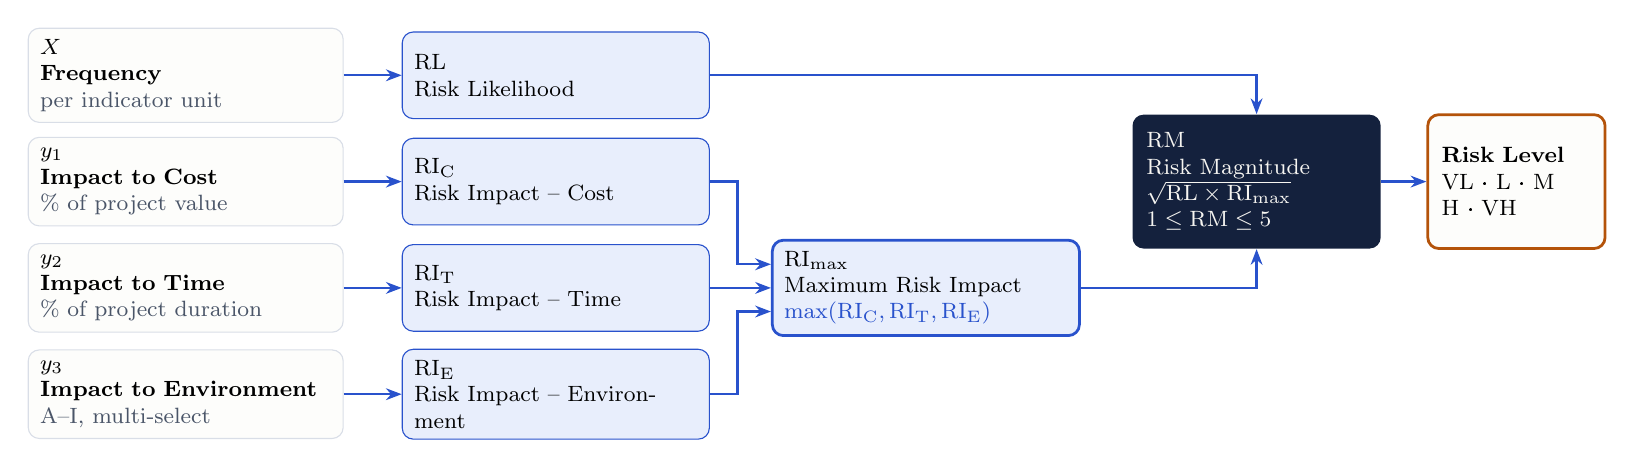
\begin{tikzpicture}[
  inp/.style={draw=line,fill=card,rounded corners=4pt,minimum width=4.0cm,minimum height=1.1cm,text width=3.7cm,align=left,inner sep=4pt,font=\footnotesize},
  scr/.style={draw=accent,fill=accentbg,rounded corners=4pt,minimum width=3.9cm,minimum height=1.1cm,text width=3.6cm,align=left,inner sep=4pt,font=\footnotesize},
  arr/.style={-{Stealth[length=2mm]},accent,thick}]
  \node[inp] (x)  at (0,0)     {$X$\\\textbf{Frequency}\\{\color{muted}per indicator unit}};
  \node[inp] (y1) at (0,-1.35) {$y_1$\\\textbf{Impact to Cost}\\{\color{muted}\% of project value}};
  \node[inp] (y2) at (0,-2.7)  {$y_2$\\\textbf{Impact to Time}\\{\color{muted}\% of project duration}};
  \node[inp] (y3) at (0,-4.05) {$y_3$\\\textbf{Impact to Environment}\\{\color{muted}A--I, multi-select}};
  \node[scr] (rl)  at (4.7,0)     {$\RL$\\Risk Likelihood};
  \node[scr] (ric) at (4.7,-1.35) {$\RIC$\\Risk Impact -- Cost};
  \node[scr] (rit) at (4.7,-2.7)  {$\RIT$\\Risk Impact -- Time};
  \node[scr] (rie) at (4.7,-4.05) {$\RIE$\\Risk Impact -- Environment};
  \node[scr,line width=1pt] (rim) at (9.4,-2.7) {$\RImax$\\Maximum Risk Impact\\{\color{accent}$\max(\RIC,\RIT,\RIE)$}};
  \node[fill=navy,text=paper,rounded corners=4pt,text width=2.8cm,minimum height=1.7cm,align=left,inner sep=5pt,font=\footnotesize]
     (rm) at (13.6,-1.35) {$\RM$\\Risk Magnitude\\$\sqrt{\RL\times\RImax}$\\$1\le\RM\le5$};
  \node[draw=warm,line width=1pt,fill=card,rounded corners=4pt,text width=1.9cm,minimum height=1.7cm,align=left,inner sep=5pt,font=\footnotesize]
     (lv) at (16.9,-1.35) {\textbf{Risk Level}\\VL · L · M\\H · VH};
  \foreach \a/\b in {x/rl,y1/ric,y2/rit,y3/rie}{\draw[arr] (\a) -- (\b);}
  \draw[arr] (ric.east) -- ++(0.35,0) |- ($(rim.west)+(0,0.3)$);
  \draw[arr] (rit.east) -- (rim.west);
  \draw[arr] (rie.east) -- ++(0.35,0) |- ($(rim.west)+(0,-0.3)$);
  \draw[arr] (rl.east) -| (rm.north);
  \draw[arr] (rim.east) -| (rm.south);
  \draw[arr] (rm) -- (lv);
\end{tikzpicture}}
\end{center}

\begin{tabularx}{\linewidth}{@{}l l X l@{}}
\toprule
Symbol & Name & Meaning & Range\\\midrule
$X$ & Frequency & How often / how much the risk event occurs: a number in the indicator's own unit (Part II) & $\ge0$\\
$y_1$ & Impact to Cost & Extra cost as \% of project value (ร้อยละมูลค่าโครงการ) & $\ge0$\\
$y_2$ & Impact to Time & Delay as \% of project duration (ร้อยละของระยะเวลาโครงการ) & $\ge0$\\
$y_3$ & Impact to Environment & Set of ticked options A--I & ---\\
$\RL$ & Risk Likelihood & Score of $X$ & 1--5\\
$\RIC,\RIT,\RIE$ & Risk Impact & Scores of $y_1$, $y_2$, $y_3$ & 1--5\\
$\RImax$ & Maximum Risk Impact & Worst of the three impact scores & 1--5\\
$\RM$ & Risk Magnitude & Combined likelihood and worst impact & 1--5\\
Level & Risk Level & VL, L, M, H, VH & ---\\
\bottomrule
\end{tabularx}

\section{Inputs}\label{sec:inp}
\subsection*{Cost and time: percentages only}
The engine accepts $y_1$ and $y_2$ \textbf{only as percentages}. Unit conversion is not part of the engine; it is noted here because the layer in front of the engine does it. The user may enter an \textbf{amount} (baht or days) or a \textbf{percentage}; since every project stores its value (มูลค่าโครงการ) and its timeframe (ระยะเวลาโครงการ), that layer converts an amount to a percentage and passes only the percentage on.

\begin{center}
\renewcommand{\arraystretch}{1.5}
\begin{tabular}{@{}l l l l@{}}
\toprule
Input & Option 1 · amount & Option 2 · percentage & Conversion (input layer, before the engine)\\\midrule
$y_1$ Impact to Cost & baht (บาท) & \% of project value & $y_1=\dfrac{\text{baht}}{\text{project value}}\times100$\\[10pt]
$y_2$ Impact to Time & days (วัน) & \% of project duration & $y_2=\dfrac{\text{days}}{\text{end date}-\text{start date}}\times100$\\
\bottomrule
\end{tabular}
\end{center}

\begin{itemize}[leftmargin=1.4em,labelwidth=1em,align=left]
\item[•] Example: project value ฿250,000,000, extra cost ฿61,100,000 $\Rightarrow y_1=24.44\%$; duration 730 days, delay 120 days $\Rightarrow y_2=16.44\%$.
\item[•] A percentage is entered as 0--100. An amount may exceed the project value or duration; the resulting percentage above the threshold $e$ simply scores 5.
\item[•] Project duration is counted in calendar days from the start date to the end date of the project.
\item[•] The input layer stores the value as entered, its unit and the converted percentage. Each assessment version keeps a snapshot of the project value and dates, so later edits to the project do not change old results.
\item[•] Enter \textbf{0} when an impact is negligible (มีผลกระทบน้อยมากให้เติม ศูนย์); it scores 1.
\end{itemize}

\subsection*{Other inputs}
\begin{itemize}[leftmargin=1.4em,labelwidth=1em,align=left]
\item[•] $X$ is a \textbf{number only}, in the indicator's own unit (Part II), and must be \textbf{0 or more} ($X\ge0$; negative values are rejected). There are no options to pick for $X$: the questionnaire's ``เลือกเพียงข้อหนึ่งข้อใด'' choice is not used, for every indicator including EC-HS-2 and EC-HS-5 (§\ref{sec:hs}).
\item[•] $y_3$ is a multi-select of options A--I (§4).
\item[•] An indicator is \emph{complete} when $X$, $y_1$, $y_2$ and $y_3$ are all given. Only complete indicators get $\RM$ and a level.
\end{itemize}

\section{Scoring \texorpdfstring{$X$, $y_1$, $y_2$}{X, y1, y2}}\label{sec:score}
Each numeric input $v$ is placed among five thresholds $a<b<c<d<e$ and scored by straight-line interpolation (the triangular membership functions written as a score):
\[
s(v)=\begin{cases}
1 & v\le a\\[2pt]
1+\dfrac{v-a}{b-a} & a<v\le b\\[8pt]
2+\dfrac{v-b}{c-b} & b<v\le c\\[8pt]
3+\dfrac{v-c}{d-c} & c<v\le d\\[8pt]
4+\dfrac{v-d}{e-d} & d<v\le e\\[2pt]
5 & v>e
\end{cases}
\qquad
\RL=s(X),\quad \RIC=s(y_1),\quad \RIT=s(y_2).
\]

\begin{tabularx}{\linewidth}{@{}l X ccccc@{}}\toprule
Score & Thresholds used & $a$ & $b$ & $c$ & $d$ & $e$\\\midrule
$\RL$ & The indicator's own set (55 sets, Part II) & \multicolumn{5}{c}{per indicator}\\
$\RIC$ & Impact Cost, shared by all indicators & 9.58 & 23.92 & 47.5 & 61.42 & 80\\
$\RIT$ & Impact Time, shared by all indicators & 13.79 & 23.33 & 46.67 & 60.83 & 79.33\\\bottomrule
\end{tabularx}

\medskip
\textbf{Rules}
\begin{itemize}[leftmargin=1.4em,labelwidth=1em,align=left]
\item[•] \textbf{Inverse indicators} (EC-MG-5, EC-CO-5, EC-RS-1, EV-EV-4): $a>b>c>d>e$, lower value means higher risk. Mirror the comparisons: $v\ge a\Rightarrow1$, $v<e\Rightarrow5$, interpolate in between.
\item[•] \textbf{Three-threshold indicators}: seven indicators have only $a,b,c$ (EC-HS-2, EC-HS-5) or only $c,d,e$ (EC-HS-1, EC-HS-3, SO-PL-1, EV-EV-2, EV-EV-3; the master's $a=b=0$ are placeholders). Their scoring is in §\ref{sec:hs}.
\item[•] Scores always stay within 1--5.
\item[•] \textbf{Rounding (configurable):} $\RL$, $\RIC$, $\RIT$, $\RIE$ are rounded to $p_s$ decimals before $\RImax$ and $\RM$; default $p_s=2$ (this reproduces the requirement deck exactly).
\end{itemize}

\section{Environmental impact \texorpdfstring{$y_3\to\RIE$}{y3 -> RI_E}}
Options A--I can be ticked together (A, ``very little impact'', is not combined with the others). Each option has a score; $\RIE$ is the highest score among the ticked options:
\[ \RIE=\max_{o\,\in\,\text{ticked}} s(o) \qquad\text{e.g. C, F, H: }\max(1,3,5)=5;\quad \text{B, C: }\max(1,1)=1 \]
\begin{tabularx}{\linewidth}{@{}cXc@{}}\toprule
Option & Effect & $s(o)$\\\midrule
A & มีผลกระทบน้อยมาก & 1 (VL)\\ B & ประสิทธิภาพของเครื่องมือ & 1 (VL)\\ C & การกองเก็บวัสดุที่ไม่สะดวกต่อการนำไปใช้ & 1 (VL)\\
D & การเพิ่มขยะ สะสมขยะ และกำจัดขยะ & 2 (L)\\ E & ขยะที่เกิดจากการรื้อถอน แยก ฝังกลบ จากขั้นตอนการก่อสร้าง & 2 (L)\\
F & มลพิษในเขตก่อสร้าง เสียง ฝุ่น กลิ่น ขยะ ดินโคลน & 3 (M)\\ G & ไม่รักษากฎระเบียบข้อบังคับท้องถิ่น เกี่ยวกับสิ่งแวดล้อม & 4 (H)\\
H & การเปลี่ยนแปลงภูมิประเทศ รอบสถานที่ และภายในพื้นที่ก่อสร้าง & 5 (VH)\\ I & น้ำท่วม ดินสไลด์ ฐานรากโครงสร้าง & 5 (VH)\\\bottomrule
\end{tabularx}

\section{Worst impact and risk magnitude}
\[ \RImax=\max(\RIC,\ \RIT,\ \RIE),\qquad \boxed{\;\RM=\sqrt{\RL\times\RImax}\;} \]
Likelihood times the worst of the three impacts; the square root keeps the result on the 1--5 scale. Because of the maximum, one severe impact is enough: an item that is cheap and on time but harms the environment still scores high.

\begin{center}\small
$\RM$ for whole-number scores ($\RL$ rows, $\RImax$ columns)\\[3pt]
\begin{tabular}{c|ccccc}
 & 1 & 2 & 3 & 4 & 5\\\hline
5 & 2.24 & 3.16 & 3.87 & 4.47 & 5.00\\
4 & 2.00 & 2.83 & 3.46 & 4.00 & 4.47\\
3 & 1.73 & 2.45 & 3.00 & 3.46 & 3.87\\
2 & 1.41 & 2.00 & 2.45 & 2.83 & 3.16\\
1 & 1.00 & 1.41 & 1.73 & 2.00 & 2.24
\end{tabular}
\end{center}

\section{Risk level}
Five triangular membership functions on $\RM$ peak at 1, 2, 3, 4 and 5. The level is the one with the highest membership; each border therefore lies halfway between two peaks.
\[ \text{level}=\arg\max_{\ell\in\{\text{VL, L, M, H, VH}\}}\mu_\ell(\RM) \]
\begin{center}
\begin{minipage}{0.56\linewidth}
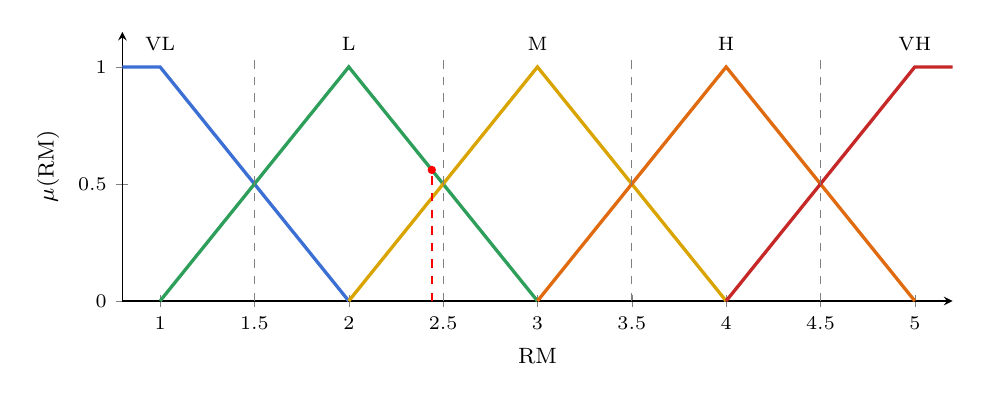
\begin{tikzpicture}
\begin{axis}[width=\linewidth,height=5cm,xmin=0.8,xmax=5.2,ymin=0,ymax=1.15,
  xtick={1,1.5,2,2.5,3,3.5,4,4.5,5},ytick={0,0.5,1},xlabel={$\RM$},ylabel={$\mu(\RM)$},
  tick label style={font=\scriptsize},label style={font=\footnotesize},axis lines=left,clip=false]
  \addplot[cVL,very thick] coordinates {(0.8,1) (1,1) (2,0)};
  \addplot[cL,very thick]  coordinates {(1,0) (2,1) (3,0)};
  \addplot[cM,very thick]  coordinates {(2,0) (3,1) (4,0)};
  \addplot[cH,very thick]  coordinates {(3,0) (4,1) (5,0)};
  \addplot[cVH,very thick] coordinates {(4,0) (5,1) (5.2,1)};
  \foreach \b in {1.5,2.5,3.5,4.5}{\edef\t{\noexpand\draw[gray,dashed] (axis cs:\b,0) -- (axis cs:\b,1.05);}\t}
  \node[font=\scriptsize] at (axis cs:1,1.1) {VL};\node[font=\scriptsize] at (axis cs:2,1.1) {L};\node[font=\scriptsize] at (axis cs:3,1.1) {M};\node[font=\scriptsize] at (axis cs:4,1.1) {H};\node[font=\scriptsize] at (axis cs:5,1.1) {VH};
  \draw[red,thick,dashed] (axis cs:2.44,0) -- (axis cs:2.44,0.56);
  \fill[red] (axis cs:2.44,0.56) circle (1.5pt);
\end{axis}
\end{tikzpicture}
\end{minipage}\hfill
\begin{minipage}{0.4\linewidth}\small
\begin{tabular}{@{}ll@{}}
\colorbox{lvVL}{\strut\ VL ต่ำมาก\ } & $1\le\RM<1.5$\\[2pt]
\colorbox{lvL}{\strut\ L ต่ำ\ }   & $1.5\le\RM<2.5$\\[2pt]
\colorbox{lvM}{\strut\ M ปานกลาง\ }   & $2.5\le\RM<3.5$\\[2pt]
\colorbox{lvH}{\strut\ H สูง\ }   & $3.5\le\RM<4.5$\\[2pt]
\colorbox{lvVH}{\strut\ VH สูงมาก\ } & $4.5\le\RM\le5$
\end{tabular}
\end{minipage}
\end{center}
\begin{itemize}[leftmargin=1.4em,labelwidth=1em,align=left]
\item[•] Example (red): $\mu_L(2.44)=0.56>\mu_M(2.44)=0.44\Rightarrow$ L.
\item[•] Exactly on a border ($\RM=1.5,2.5,3.5,4.5$, memberships $0.5/0.5$): the \textbf{higher} level.
\item[•] \textbf{Rounding (configurable):} $\RM$ is rounded to $p_m$ decimals, default $p_m=3$, and the rounded value is classified.
\end{itemize}

\section{Advice: when and which list to show}\label{sec:adv}
Each indicator carries four expert advice lists (คำแนะนำลดความเสี่ยงจากผู้เชี่ยวชาญ, sheet \texttt{Indenti.8.11.26}), named after the score they target: $\RL$, $\RIC$, $\RIT$, $\RIE$. Each is an ordered list of \textbf{1 to 5 measures} (three per list in the current sheet; the count can differ between lists), printed in Part II.

\textbf{When.} Advice is shown only for an indicator whose level is \textbf{H or VH} ($\RM\ge3.5$). VL, L and M show none.

\textbf{Which.} One list, picked by comparing the two factors of $\RM=\sqrt{\RL\times\RImax}$: whichever is larger is the one to bring down.
\[
\text{advice}=\begin{cases}
\text{none} & \text{level}\in\{\text{VL, L, M}\}\\[2pt]
\RL\ \text{list (reduce likelihood)} & \text{level}\in\{\text{H, VH}\},\ \RL\ge\RImax\\[2pt]
\RIC\ \text{list (reduce cost impact)} & \text{level}\in\{\text{H, VH}\},\ \RL<\RImax=\RIC\\[2pt]
\RIT\ \text{list (reduce time impact)} & \text{level}\in\{\text{H, VH}\},\ \RL<\RImax=\RIT\\[2pt]
\RIE\ \text{list (reduce environmental impact)} & \text{level}\in\{\text{H, VH}\},\ \RL<\RImax=\RIE
\end{cases}
\]
\begin{center}\small
\begin{tabularx}{\linewidth}{@{}l l X@{}}
\toprule
List & Source column header & Shown when (level H or VH, and \dots)\\\midrule
$\RL$  & RL & $\RL\ge\RImax$ (likelihood drives the risk, or ties with the worst impact)\\
$\RIC$ & ผลกระทบด้านต้นทุน RIC & $\RL<\RImax$, worst impact is cost\\
$\RIT$ & ผลกระทบด้าน เวลา RIT & $\RL<\RImax$, worst impact is time\\
$\RIE$ & ผลกระทบด้านสิ่งแวดล้อม RIE & $\RL<\RImax$, worst impact is environment\\
\bottomrule
\end{tabularx}
\end{center}
\begin{itemize}[leftmargin=1.4em,labelwidth=1em,align=left]
\item[•] Compare the rounded scores ($p_s$ decimals), the same values that go into $\RM$.
\item[•] $\RL=\RImax$ counts as $\RL\ge\RImax$: the $\RL$ list.
\item[•] \textbf{Ties between impacts} (and $\RL<\RImax$): show \textbf{every} list whose impact equals $\RImax$, two or three, in the order $\RIC$, $\RIT$, $\RIE$.
\end{itemize}
\begin{center}\small
\renewcommand{\arraystretch}{1.2}
\begin{tabular}{@{}cccc c c c l@{}}
\toprule
$\RL$ & $\RIC$ & $\RIT$ & $\RIE$ & $\RImax$ & $\RM$ & Level & Advice shown\\\midrule
5.00 & 4.00 & 2.00 & 1 & 4.00 & 4.472 & H & $\RL$\\
4.00 & 4.00 & 1.00 & 1 & 4.00 & 4.000 & H & $\RL$ (tie goes to $\RL$)\\
2.45 & 2.02 & 3.10 & 5 & 5 & 3.500 & H & $\RIE$ (worked example, §\ref{sec:ex})\\
3.00 & 5.00 & 5.00 & 5 & 5 & 3.873 & H & $\RIC$, $\RIT$ and $\RIE$ (three-way tie)\\
4.00 & 2.00 & 5.00 & 5 & 5 & 4.472 & H & $\RIT$ and $\RIE$ (two-way tie)\\
2.00 & 3.00 & 1.00 & 1 & 3.00 & 2.449 & L & none\\
\bottomrule
\end{tabular}
\end{center}

\section{Indicators with three thresholds}\label{sec:hs}
Seven indicators have only three of the five thresholds. The two groups mirror each other: one has no $d,e$ and skips H; the other has no $a,b$ and skips L. $v$ is the value of $X$ ($v\ge0$).

\subsection*{Only $a,b,c$: EC-HS-2, EC-HS-5 \quad ($\RL$ levels VL, L, M, VH)}
$X$ is the number of treatment days (จำนวนวันในการรักษา).
\[
\RL=\begin{cases}
1 & v\le a\\[2pt]
1+\dfrac{v-a}{b-a} & a<v\le b\\[8pt]
2+\dfrac{v-b}{c-b} & b<v\le c\\[8pt]
5 & v>c
\end{cases}
\]
\subsection*{Only $c,d,e$: EC-HS-1, EC-HS-3, SO-PL-1, EV-EV-2, EV-EV-3 \quad ($\RL$ levels VL, M, H, VH)}
\[
\RL=\begin{cases}
1 & v<c\\[2pt]
3+\dfrac{v-c}{d-c} & c\le v\le d\\[8pt]
4+\dfrac{v-d}{e-d} & d<v\le e\\[8pt]
5 & v>e
\end{cases}
\]
\begin{center}\small
\begin{tabular}{@{}l l ccccc@{}}
\toprule
Group ID & Indicator & $a$ & $b$ & $c$ & $d$ & $e$\\\midrule
EC-HS-2 & Poor safety management & 0.92 & 2.96 & 4.88 & --- & ---\\
EC-HS-5 & Fatalities & 4.58 & 10 & 15.71 & --- & ---\\\midrule
EC-HS-1 & Inadequate safety measures & --- & --- & 1.33 & 3.54 & 4.42\\
EC-HS-3 & Strict health \& safety regulations & --- & --- & 1.21 & 2.88 & 4.17\\
SO-PL-1 & Changes in legislation & --- & --- & 3 & 9.17 & 9.83\\
EV-EV-2 & Construction pollution & --- & --- & 1.33 & 3.33 & 4.08\\
EV-EV-3 & Strict environmental regulations & --- & --- & 1.33 & 3.33 & 4.08\\
\bottomrule
\end{tabular}
\end{center}
\begin{itemize}[leftmargin=1.4em,labelwidth=1em,align=left]
\item[•] Only $a,b,c$: above $c$, $\RL$ jumps from 3 to 5 (no H). Only $c,d,e$: below $c$, $\RL=1$, and at $c$ it jumps to 3 (no L).
\item[•] $v=c$ scores 3 in both groups.
\item[•] The missing thresholds are stored as empty (not 0). $y_1$, $y_2$, $y_3$ are entered and scored as for every other indicator.
\end{itemize}

\section{Worked example · EC-MG-2}\label{sec:ex}
การวางแผนโครงการ และการจัดทำงบประมาณ — inputs from requirement deck page 11.

\begin{center}
\renewcommand{\arraystretch}{1.3}
\begin{tabular}{@{}l c l c c@{}}
\toprule
Input $\to$ score & Value & $a$ -- $e$ & Calculation & Score\\\midrule
$X\to\RL$ & 8.68 & 2.96 · 6.71 · 11.04 · 16 · 20 & $2+\dfrac{8.68-6.71}{11.04-6.71}$ & \textbf{2.45}\\[8pt]
$y_1\to\RIC$ & 24.44 & 9.58 · 23.92 · 47.5 · 61.42 · 80 & $2+\dfrac{24.44-23.92}{47.5-23.92}$ & \textbf{2.02}\\[8pt]
$y_2\to\RIT$ & 48.03 & 13.79 · 23.33 · 46.67 · 60.83 · 79.33 & $3+\dfrac{48.03-46.67}{60.83-46.67}$ & \textbf{3.10}\\[8pt]
$y_3\to\RIE$ & C, F, H & option scores 1, 3, 5 & $\max(1,3,5)$ & \textbf{5}\\
\bottomrule
\end{tabular}
\[ \RImax=\max(2.02,\ 3.10,\ 5)=5,\qquad \RM=\sqrt{2.45\times5}=3.500\ \Rightarrow\ \text{H (on the M/H border, goes up)} \]
\end{center}
\textbf{Advice:} the level is H, so advice is shown; $\RL=2.45<\RImax=5$ and the maximum comes from $\RIE$, so the $\RIE$ list is shown:
\begin{enumerate}[leftmargin=2em]
\item จัดสรรงบประมาณเฉพาะสำหรับมาตรการป้องกันสิ่งแวดล้อม
\item รวมต้นทุนด้านสิ่งแวดล้อมในแผนงบประมาณตั้งแต่เริ่มต้น
\item กำหนดแผนฉุกเฉินด้านสิ่งแวดล้อมเมื่อต้องตัดลดงบประมาณ
\end{enumerate}

\section{Decisions and open points}
\begin{tabularx}{\linewidth}{@{}l X l@{}}
\toprule
Date & Decision & By\\\midrule
21 Oct & $\RIE$ = highest option score (not the count rule) & Tae\\
21 Oct & Level = RM membership functions (borders 1.5 / 2.5 / 3.5 / 4.5) & Tae\\
8 Nov & Advice list: $\RL$ list if $\RL\ge\RImax$, otherwise the list of the impact that gives $\RImax$ (§\ref{sec:adv}) & Expert\\
8 Nov & Advice shown only at level H or VH & Tae\\
10 Nov & EC-HS-2 / EC-HS-5: thresholds $a$, $b$, $c$ only (no $d$, $e$); $\RL=5$ above $c$; treatment days only (event mode of 29 Oct dropped) & Tae\\
10 Nov & $X$ is a number only (no options), $X\ge0$ & Tae\\
11 Nov & Advice: when impacts tie for $\RImax$, show every tied list & Expert\\
11 Nov & $a=b=0$ indicators: only $c,d,e$; $\RL$ levels VL, M, H, VH (mirror of EC-HS-2/5); $v=c$ scores 3 & Expert, Tae\\
11 Nov & Rounding configurable: scores $p_s=2$, $\RM$ $p_m=3$ by default & Tae\\
11 Nov & Unit conversion of $y_1$, $y_2$ is done by the input layer; the engine takes \% only & Tae\\
15 Nov & v1.1: $y_1$, $y_2$ questions keep the note [มีผลกระทบ น้อยมากให้เติม ศูนย์] & Tae\\
15 Nov & v1.1: questions aligned with the 15 Nov questionnaire; EV-EV-4 renamed การร้องเรียนเนื่องจากการกำจัดขยะก่อสร้างที่ผิดกฎหมาย (was การดำเนินคดี…) & Tae\\
15 Nov & EC-TC-4: $X$ unit is per project period (ต่อระยะเวลาโครงการ) & Tae\\
\midrule
Open & Tie rule on level borders (higher level) to confirm & \\
\bottomrule
\end{tabularx}

\clearpage\part{Indicators}
\section{How to read Part II}
Each indicator is identified by a \textbf{group ID} (e.g.\ EC-MG-1: dimension–factor–number), shown in the app, and by its legacy \textbf{F-code} from the research (e.g.\ F11), kept for data and traceability. The 55 indicators sit in \textbf{11 factors} grouped into \textbf{3 dimensions}: Economic (EC), Social (SO) and Environmental (EV). Factor numbers follow the 24 Oct master (ordered by dimension); the F-code prefix keeps the research numbering.

\begin{tabularx}{\linewidth}{@{}>{\bfseries}p{3.2cm}X@{}}
\toprule
Field & Meaning\\\midrule
Likelihood unit & What $X$ measures for this indicator (the respondent enters this number).\\
Thresholds $a$--$e$ & Scale used to turn $X$ into $\RL$ (1--5), see §\ref{sec:score}. \emph{Inverse}: lower $X$ = higher risk ($a>e$). EC-HS-2 and EC-HS-5 have $a$, $b$, $c$ only; EC-HS-1, EC-HS-3, SO-PL-1, EV-EV-2, EV-EV-3 have $c$, $d$, $e$ only (§\ref{sec:hs}).\\
Input & Always a number, 0 or more ($X\ge0$), §\ref{sec:inp}. No options: the questionnaire's เลือกเพียงข้อหนึ่งข้อใด choice is not used.\\
Questions & Questionnaire wording (sheet คำถาม, 15 Nov; obvious typos corrected), one per input (for $X$ the numeric question, with the pick-one tag removed): $X$ (frequency $\to\RL$), $y_1$ (cost $\to\RIC$), $y_2$ (time $\to\RIT$), $y_3$ (environment $\to\RIE$); \blank{} marks a value to fill in. For $y_1$ and $y_2$ the trailing unit instruction (โปรดระบุ ร้อยละ … หรือ … บาท / ระบุร้อยละ … วัน) is cut: the user picks baht or \%, days or \% (§\ref{sec:inp}); the note [มีผลกระทบ น้อยมากให้เติม ศูนย์] is kept, so the user enters 0 for a negligible impact.\\
Expert advice & Four lists of 1--5 measures each (three each in sheet Indenti.8.11.26, verbatim): $\RL$, $\RIC$, $\RIT$, $\RIE$. Shown only at level H or VH; then one list, chosen by the rule in §\ref{sec:adv}. The condition is printed next to each list.\\
\bottomrule
\end{tabularx}

\section{Structure: dimensions and factors}
\small
\begin{tabularx}{\linewidth}{@{}c l X l l l c@{}}
\toprule
No. & Factor & Thai & Group ID & Research & Indicators & n\\\midrule
\rowcolor{ECbg}\multicolumn{7}{@{}p{\dimexpr\linewidth\relax}@{}}{\textbf{\color{ECfg}ECONOMIC (EC) · ด้านเศรษฐกิจ}\hfill{\color{muted}5 factors · 25 indicators}}\\
1 & Management & ด้านการจัดการ & EC-MG & F1 & EC-MG-[1-5] & 5\\
2 & Technic & ด้านทางเทคนิค & EC-TC & F2 & EC-TC-[1-5] & 5\\
3 & Construction & ด้านการก่อสร้าง & EC-CO & F3 & EC-CO-[1-5] & 5\\
4 & Resource & ด้านทรัพยากรที่เกี่ยวข้อง & EC-RS & F4 & EC-RS-[1-5] & 5\\
5 & Health and safety & ด้านสุขภาพและความปลอดภัย & EC-HS & F11 & EC-HS-[1-5] & 5\\
\rowcolor{SCbg}\multicolumn{7}{@{}p{\dimexpr\linewidth\relax}@{}}{\textbf{\color{SCfg}SOCIAL (SO) · ด้านสังคม}\hfill{\color{muted}4 factors · 20 indicators}}\\
6 & Contract and law & ด้านตามสัญญาและกฎหมาย & SO-CL & F6 & SO-CL-[1-5] & 5\\
7 & Economy and finance & ด้านเศรษฐกิจและการเงิน & SO-EF & F7 & SO-EF-[1-5] & 5\\
8 & Society & ด้านสังคม & SO-SO & F8 & SO-SO-[1-5] & 5\\
9 & Politic & ด้านทางการเมือง & SO-PL & F9 & SO-PL-[1-5] & 5\\
\rowcolor{EVbg}\multicolumn{7}{@{}p{\dimexpr\linewidth\relax}@{}}{\textbf{\color{EVfg}ENVIRONMENTAL (EV) · ด้านสิ่งแวดล้อม}\hfill{\color{muted}2 factors · 10 indicators}}\\
10 & Site conditions & ด้านเงื่อนไขของไซต์ & EV-SC & F5 & EV-SC-[1-5] & 5\\
11 & Environmental & ด้านสิ่งแวดล้อม & EV-EV & F10 & EV-EV-[1-5] & 5\\
\midrule
 & \textbf{Total} & & & & & \textbf{55}\\
\bottomrule
\end{tabularx}
\normalsize

\clearpage\section{All indicators at a glance}
\subsection*{Economic (EC) · ด้านเศรษฐกิจ}\addcontentsline{toc}{subsection}{Economic (EC)}
\begin{tcolorbox}[colback=ECbg,colframe=ECfg,boxrule=0pt,leftrule=4pt,arc=0pt,left=8pt,top=4pt,bottom=4pt]{\normalsize\bfseries\color{ECfg}ECONOMIC (EC) · ด้านเศรษฐกิจ}\hfill{\small\color{muted}5 factors · 25 indicators}\end{tcolorbox}
\footnotesize
\begin{longtable}{@{}l l p{4.2cm} p{3.3cm} rrrrr c@{}}
\toprule
Group ID & F & Indicator & Likelihood unit & $a$ & $b$ & $c$ & $d$ & $e$ & \\\midrule\endhead
\bottomrule\endfoot
\multicolumn{10}{@{}l}{\textbf{\color{ECfg}1 · Management} \color{muted}ด้านการจัดการ}\\
EC-MG-1 & F11 & Poor coordination & No. of events/month & 1.21 & 2.71 & 4.54 & 7.21 & 8.92 & \\
EC-MG-2 & F12 & Inadequate planning/budgeting & \% of budget & 2.96 & 6.71 & 11.04 & 16 & 20 & \\
EC-MG-3 & F13 & Poor relationships & No. of events/month & 1.21 & 2.42 & 5.29 & 8.08 & 9.17 & \\
EC-MG-4 & F14 & Poor quality management & \% of plan & 1.96 & 3.08 & 5.33 & 8.21 & 9.92 & \\
EC-MG-5 & F15 & Poor capability of owner & No. of years & 9.33 & 8.67 & 5.88 & 3 & 2.58 & $\downarrow$\\
\multicolumn{10}{@{}l}{\textbf{\color{ECfg}2 · Technic} \color{muted}ด้านทางเทคนิค}\\
EC-TC-1 & F21 & Design errors & No. of events/period & 0 & 2.83 & 5.42 & 8.04 & 8.96 & \\
EC-TC-2 & F22 & Unanticipated design changes & No. of events/period & 0 & 2.83 & 5.42 & 8.04 & 8.96 & \\
EC-TC-3 & F23 & Incomplete design & No. of events/period & 0 & 2.67 & 5.38 & 8.08 & 9.08 & \\
EC-TC-4 & F24 & Design complexity & No. of events/project period & 0 & 2.67 & 5.38 & 8.08 & 9.08 & \\
EC-TC-5 & F25 & Poor constructability & \% of total work & 5.08 & 6.5 & 10.29 & 14.92 & 19.17 & \\
\multicolumn{10}{@{}l}{\textbf{\color{ECfg}3 · Construction} \color{muted}ด้านการก่อสร้าง}\\
EC-CO-1 & F31 & Delays causing cost increase & \% of remaining project time & 3.71 & 6.58 & 10.75 & 15.58 & 18.08 & \\
EC-CO-2 & F32 & Contractor incompetence & No. of remaining project days & 3.58 & 7.54 & 14.38 & 23.67 & 28.58 & \\
EC-CO-3 & F33 & Improper construction methods & No. of remaining project days & 1.42 & 3.33 & 6.96 & 11.88 & 15.83 & \\
EC-CO-4 & F34 & Interface conflicts & No. of events/month & 1.21 & 2.96 & 4.92 & 7 & 9 & \\
EC-CO-5 & F35 & Poor workmanship/rework & \% of work completed & 84.17 & 79.54 & 69.13 & 57.25 & 49.38 & $\downarrow$\\
\multicolumn{10}{@{}l}{\textbf{\color{ECfg}4 · Resource} \color{muted}ด้านทรัพยากรที่เกี่ยวข้อง}\\
EC-RS-1 & F41 & Shortage of skilled labour & \% of work completed & 90.42 & 85.21 & 73.33 & 60.21 & 36.25 & $\downarrow$\\
EC-RS-2 & F42 & Shortage of materials & \% of remaining time & 2.79 & 6.25 & 10.17 & 15.5 & 16.5 & \\
EC-RS-3 & F43 & Low labour productivity & \% of remaining time & 3.46 & 6 & 10.17 & 15.5 & 18.5 & \\
EC-RS-4 & F44 & Subcontractor failure & No. of remaining project days & 2 & 6.58 & 13.5 & 22.63 & 27.08 & \\
EC-RS-5 & F45 & Shortage of qualified subcontractors & No. of remaining project days & 2 & 6.21 & 12.42 & 20.71 & 25 & \\
\multicolumn{10}{@{}l}{\textbf{\color{ECfg}5 · Health and safety} \color{muted}ด้านสุขภาพและความปลอดภัย}\\
EC-HS-1 & F111 & Inadequate safety measures & No. of events/project period & --- & --- & 1.33 & 3.54 & 4.42 & \\
EC-HS-2 & F112 & Poor safety management & No. of days/project period & 0.92 & 2.96 & 4.88 & --- & --- & \\
EC-HS-3 & F113 & Strict health \& safety regulations & No. of events/project period & --- & --- & 1.21 & 2.88 & 4.17 & \\
EC-HS-4 & F114 & Changes in labour safety laws & No. of document points & 0.46 & 1.83 & 4.42 & 7.29 & 8.67 & \\
EC-HS-5 & F115 & Fatalities & No. of treatment days & 4.58 & 10 & 15.71 & --- & --- & \\
\end{longtable}\normalsize
\subsection*{Social (SO) · ด้านสังคม}\addcontentsline{toc}{subsection}{Social (SO)}
\begin{tcolorbox}[colback=SCbg,colframe=SCfg,boxrule=0pt,leftrule=4pt,arc=0pt,left=8pt,top=4pt,bottom=4pt]{\normalsize\bfseries\color{SCfg}SOCIAL (SO) · ด้านสังคม}\hfill{\small\color{muted}4 factors · 20 indicators}\end{tcolorbox}
\footnotesize
\begin{longtable}{@{}l l p{4.2cm} p{3.3cm} rrrrr c@{}}
\toprule
Group ID & F & Indicator & Likelihood unit & $a$ & $b$ & $c$ & $d$ & $e$ & \\\midrule\endhead
\bottomrule\endfoot
\multicolumn{10}{@{}l}{\textbf{\color{SCfg}6 · Contract and law} \color{muted}ด้านตามสัญญาและกฎหมาย}\\
SO-CL-1 & F61 & Contractual inconsistencies & No. of correction points/contract & 0.42 & 1.75 & 4.33 & 7.5 & 9 & \\
SO-CL-2 & F62 & Scope changes & No. of correction points/contract & 0.46 & 1.75 & 4.33 & 7.5 & 9 & \\
SO-CL-3 & F63 & Unreliable legal system & No. of correction points/contract & 0.42 & 1.75 & 4.33 & 7.5 & 9 & \\
SO-CL-4 & F64 & Code/regulation changes & No. of correction points/contract & 0.42 & 1.75 & 4.33 & 7.5 & 9 & \\
SO-CL-5 & F65 & Excessive contract variation & No. of correction points/contract & 0.46 & 1.75 & 4.33 & 7.5 & 9 & \\
\multicolumn{10}{@{}l}{\textbf{\color{SCfg}7 · Economy and finance} \color{muted}ด้านเศรษฐกิจและการเงิน}\\
SO-EF-1 & F71 & Inflation rate changes & \% of budget & 1.88 & 5.71 & 9.08 & 14.92 & 17.5 & \\
SO-EF-2 & F72 & Funding problems & \% of budget & 2.08 & 5.63 & 9 & 14.83 & 17.42 & \\
SO-EF-3 & F73 & Adverse economic conditions & \% of budget & 1.88 & 5.63 & 9 & 14.83 & 17.42 & \\
SO-EF-4 & F74 & Market demand changes & \% of budget & 2.08 & 5.63 & 9 & 14.83 & 17.42 & \\
SO-EF-5 & F75 & Economic crises & \% of budget & 2.08 & 5.63 & 9 & 14.83 & 17.42 & \\
\multicolumn{10}{@{}l}{\textbf{\color{SCfg}8 · Society} \color{muted}ด้านสังคม}\\
SO-SO-1 & F81 & Land acquisition problems & \% of remaining time & 3.67 & 6.46 & 10.92 & 16.33 & 19.33 & \\
SO-SO-2 & F82 & Public opposition & No. of days/month & 0 & 2.29 & 4 & 6.25 & 7.25 & \\
SO-SO-3 & F83 & Cultural differences & No. of events/month & 0 & 1.75 & 4.08 & 6.42 & 7.25 & \\
SO-SO-4 & F84 & Poor public relations & No. of events/month & 0 & 1.42 & 4.08 & 6.5 & 8.08 & \\
SO-SO-5 & F85 & Adverse social environment & No. of events/defined period & 0 & 1.67 & 2.58 & 3.42 & 4.25 & \\
\multicolumn{10}{@{}l}{\textbf{\color{SCfg}9 · Politic} \color{muted}ด้านทางการเมือง}\\
SO-PL-1 & F91 & Changes in legislation & No. of stop-work days & --- & --- & 3 & 9.17 & 9.83 & \\
SO-PL-2 & F92 & Permit delays or refusals & \% of remaining time & 3.67 & 6.75 & 11.71 & 17.38 & 20.46 & \\
SO-PL-3 & F93 & Government intervention & \% of remaining sub-plan & 2 & 5.92 & 10.25 & 14.92 & 18.17 & \\
SO-PL-4 & F94 & Restrictions on foreign companies & \% of remaining sub-plan & 1.5 & 5.92 & 10.25 & 14.92 & 18.17 & \\
SO-PL-5 & F95 & Differential taxation & \% of remaining sub-plan & 2.29 & 6.21 & 11.04 & 16.08 & 19.17 & \\
\end{longtable}\normalsize
\subsection*{Environmental (EV) · ด้านสิ่งแวดล้อม}\addcontentsline{toc}{subsection}{Environmental (EV)}
\begin{tcolorbox}[colback=EVbg,colframe=EVfg,boxrule=0pt,leftrule=4pt,arc=0pt,left=8pt,top=4pt,bottom=4pt]{\normalsize\bfseries\color{EVfg}ENVIRONMENTAL (EV) · ด้านสิ่งแวดล้อม}\hfill{\small\color{muted}2 factors · 10 indicators}\end{tcolorbox}
\footnotesize
\begin{longtable}{@{}l l p{4.2cm} p{3.3cm} rrrrr c@{}}
\toprule
Group ID & F & Indicator & Likelihood unit & $a$ & $b$ & $c$ & $d$ & $e$ & \\\midrule\endhead
\bottomrule\endfoot
\multicolumn{10}{@{}l}{\textbf{\color{EVfg}10 · Site conditions} \color{muted}ด้านเงื่อนไขของไซต์}\\
EV-SC-1 & F51 & Adverse subsurface conditions & \% of remaining sub-plan & 2.08 & 5.67 & 10.58 & 14.83 & 18.25 & \\
EV-SC-2 & F52 & Unforeseen site conditions & \% of remaining sub-plan & 2 & 5.75 & 10.29 & 15.25 & 19.08 & \\
EV-SC-3 & F53 & Lack of utilities/infrastructure & No. of remaining project days & 0.5 & 3.13 & 6.92 & 11.88 & 15.33 & \\
EV-SC-4 & F54 & Late site possession & \% of remaining sub-plan & 2 & 6.25 & 11.08 & 15.75 & 19.17 & \\
EV-SC-5 & F55 & Subsurface water conditions & No. of events/project & 0 & 0.5 & 1.54 & 3.96 & 5.17 & \\
\multicolumn{10}{@{}l}{\textbf{\color{EVfg}11 · Environmental} \color{muted}ด้านสิ่งแวดล้อม}\\
EV-EV-1 & F101 & Adverse environmental impacts & No. of events/project & 0 & 0.79 & 2.13 & 3.88 & 5.17 & \\
EV-EV-2 & F102 & Construction pollution & No. of events/project & --- & --- & 1.33 & 3.33 & 4.08 & \\
EV-EV-3 & F103 & Strict environmental regulations & No. of events/project & --- & --- & 1.33 & 3.33 & 4.08 & \\
EV-EV-4 & F104 & Waste disposal complaints & \% per project & 64.25 & 49.38 & 38.46 & 23.58 & 16.5 & $\downarrow$\\
EV-EV-5 & F105 & Failure to obtain environmental approval & No. of stop-work days & 0.29 & 3.17 & 7.92 & 12.75 & 17.08 & \\
\end{longtable}\normalsize
{\small\color{muted} $\downarrow$ = inverse scale (lower value = higher risk). --- = no threshold (EC-HS-2, EC-HS-5: $a,b,c$ only; EC-HS-1, EC-HS-3, SO-PL-1, EV-EV-2, EV-EV-3: $c,d,e$ only). Every $X$ is a number $\ge0$.}
\newpage
\section{Economic (EC) · ด้านเศรษฐกิจ — indicator details}
\begin{tcolorbox}[colback=ECbg,colframe=ECfg,boxrule=0pt,leftrule=4pt,arc=0pt,left=8pt,top=4pt,bottom=4pt]{\large\bfseries\color{ECfg}ECONOMIC (EC) · ด้านเศรษฐกิจ}\hfill{\small\color{muted}5 factors · 25 indicators}\end{tcolorbox}
\subsection*{1 · Management — ด้านการจัดการ {\normalsize\color{muted}(Economic, research F1)}}\addcontentsline{toc}{subsection}{1 · Management — ด้านการจัดการ}
\begin{indicator}{EC-MG-1 \,·\, F11 \quad การประสานงานที่ไม่ดีระหว่างฝ่ายต่างๆ ที่เกี่ยวข้อง}
{\color{muted}\itshape Poor coordination}\par\smallskip
\begin{tabularx}{\linewidth}{@{}p{2.9cm}X@{}}
\field{Likelihood unit} & No. of events/month \;/\; จำนวนครั้งต่อเดือน\\
\field{Thresholds} & $a=1.21,\ b=2.71,\ c=4.54,\ d=7.21,\ e=8.92$ \quad {\color{muted}\small normal (higher value = higher risk)}\\
\field{Input} & Number, $\ge0$\\
\end{tabularx}
\smallskip\par\field{Questionnaire — the question asked for each input}\vspace{2pt}
\begin{itemize}
\item[$X$] โอกาสที่จะเกิด การประสานงานที่ไม่ดีระหว่างฝ่ายต่างๆ ที่เกี่ยวข้อง จำนวน\blank{}ครั้งที่ผิดพลาดต่อเดือน
\item[$y_1$] ผลกระทบ (ด้านการเงิน) การประสานงานที่ไม่ดีระหว่างฝ่ายต่างๆที่เกี่ยวข้อง ส่งผลกระทบต่อ การเบิกจ่ายเงินไม่เป็นไปตามผลงาน [มีผลกระทบ น้อยมากให้เติม ศูนย์]
\item[$y_2$] ผลกระทบ (ด้านเวลา) ความล่าช้าจากการประสานงานที่ไม่ดีระหว่างฝ่ายต่างๆที่เกี่ยวข้อง [มีผลกระทบ น้อยมากให้เติม ศูนย์]
\item[$y_3$] ผลกระทบ (ด้านสิ่งแวดล้อม)จาก การประสานงานที่ไม่ดีระหว่างฝ่ายต่างๆที่เกี่ยวข้อง ความยั่งยืนด้านสิ่งแวดล้อม (เลือกได้หลายข้อ)
\end{itemize}
\smallskip\par\field{Expert advice (คำแนะนำลดความเสี่ยงจากผู้เชี่ยวชาญ) — shown only at level H or VH, one list, §\ref{sec:adv}}\par\vspace{3pt}
\begin{tabularx}{\linewidth}{@{}>{\raggedright\arraybackslash}X@{\hspace{14pt}}>{\raggedright\arraybackslash}X@{}}
\advhead{$\RL$ · likelihood}{$\RL\ge\RImax$}\advitem{1}{จัดตั้งหน่วยประสานงานเฉพาะสำหรับโครงการเกาะ}\advitem{2}{จัดการประชุมประสานงานหลายฝ่ายเป็นประจำ}\advitem{3}{มอบหมายหน่วยงานประสานงานในสถานที่เพียงคนเดียว} & \advhead{$\RIC$ · cost}{$\RL<\RImax=\RIC$}\advitem{1}{กำหนดงบประมาณสำรองสำหรับงานแก้ไขจากความผิดพลาดในการประสานงาน}\advitem{2}{ใช้ระบบติดตามต้นทุนแบบเรียลไทม์เพื่อตรวจจับค่าใช้จ่ายที่เกิดจากความล่าช้าในการประสานงาน}\advitem{3}{จัดทำขั้นตอนอนุมัติค่าใช้จ่ายฉุกเฉินเมื่อเกิดปัญหาการประสานงาน}\\[5pt]
\advhead{$\RIT$ · time}{$\RL<\RImax=\RIT$}\advitem{1}{จัดทำแผนงานสำรองสำหรับกิจกรรมที่ต้องพึ่งพาการประสานงานระหว่างฝ่าย}\advitem{2}{กำหนดเวลาบัฟเฟอร์ในแผนงานสำหรับจุดที่ต้องประสานงาน}\advitem{3}{ใช้ระบบแจ้งเตือนอัตโนมัติเมื่อกิจกรรมล่าช้าจากการรอประสานงาน} & \advhead{$\RIE$ · environment}{$\RL<\RImax=\RIE$}\advitem{1}{กำหนดผู้รับผิดชอบด้านสิ่งแวดล้อมในทุกฝ่ายที่เกี่ยวข้อง}\advitem{2}{บูรณาการข้อกำหนดด้านสิ่งแวดล้อมเข้าในทุกขั้นตอนการประสานงาน}\advitem{3}{จัดทำรายงานผลกระทบสิ่งแวดล้อมร่วมกันระหว่างฝ่ายเมื่อเกิดปัญหาการประสานงาน}\\
\end{tabularx}
\end{indicator}
\medskip
\begin{indicator}{EC-MG-2 \,·\, F12 \quad การวางแผนโครงการ และการจัดทำงบประมาณไม่เพียงพอ หรือไม่ดี}
{\color{muted}\itshape Inadequate planning/budgeting}\par\smallskip
\begin{tabularx}{\linewidth}{@{}p{2.9cm}X@{}}
\field{Likelihood unit} & \% of budget \;/\; ความคลาดเคลื่อนร้อยละ ของงบประมาณโครงการ\\
\field{Thresholds} & $a=2.96,\ b=6.71,\ c=11.04,\ d=16,\ e=20$ \quad {\color{muted}\small normal (higher value = higher risk)}\\
\field{Input} & Number, $\ge0$\\
\end{tabularx}
\smallskip\par\field{Questionnaire — the question asked for each input}\vspace{2pt}
\begin{itemize}
\item[$X$] โอกาสที่จะเกิด การวางแผนโครงการ และการจัดทำงบประมาณที่ไม่เพียงพอหรือไม่ดี ความคลาดเคลื่อนร้อยละ \blank{}ของงบประมาณโครงการ
\item[$y_1$] ผลกระทบ(ด้านการเงิน) การวางแผนโครงการ และการจัดทำงบประมาณที่ไม่เพียงพอหรือไม่ดี ส่งผลกระทบต่อ การเบิกจ่ายเงินไม่เป็นไปตามผลงาน [มีผลกระทบ น้อยมากให้เติม ศูนย์]
\item[$y_2$] ผลกระทบ (ด้านเวลา) ความล่าช้าจากการวางแผนโครงการ และการจัดทำงบประมาณที่ไม่เพียงพอหรือไม่ดี [มีผลกระทบ น้อยมากให้เติม ศูนย์]
\item[$y_3$] ผลกระทบ (ด้านสิ่งแวดล้อม) จากการวางแผนโครงการ และการจัดทำงบประมาณที่ไม่เพียงพอหรือไม่ดี ความยั่งยืนด้านสิ่งแวดล้อม (เลือกได้หลายข้อ)
\end{itemize}
\smallskip\par\field{Expert advice (คำแนะนำลดความเสี่ยงจากผู้เชี่ยวชาญ) — shown only at level H or VH, one list, §\ref{sec:adv}}\par\vspace{3pt}
\begin{tabularx}{\linewidth}{@{}>{\raggedright\arraybackslash}X@{\hspace{14pt}}>{\raggedright\arraybackslash}X@{}}
\advhead{$\RL$ · likelihood}{$\RL\ge\RImax$}\advitem{1}{แก้ไขการวางแผนโครงการด้วยข้อจำกัดเฉพาะเกาะ}\advitem{2}{แนะนำเบี้ยเลี้ยงฉุกเฉินสำหรับโลจิสติกส์ และสภาพอากาศ}\advitem{3}{เสริมสร้างกลไกการตรวจสอบ และควบคุมต้นทุน} & \advhead{$\RIC$ · cost}{$\RL<\RImax=\RIC$}\advitem{1}{จัดทำแผนการเงินฉุกเฉินเมื่อต้นทุนเกินงบประมาณ}\advitem{2}{เจรจาสัญญาราคาคงที่กับซัพพลายเออร์หลักเพื่อควบคุมต้นทุน}\advitem{3}{ใช้ระบบเตือนภัยล่วงหน้าเมื่อค่าใช้จ่ายเกินเกณฑ์ที่กำหนด}\\[5pt]
\advhead{$\RIT$ · time}{$\RL<\RImax=\RIT$}\advitem{1}{จัดทำแผนเร่งรัดงานเมื่อโครงการล่าช้าจากปัญหางบประมาณ}\advitem{2}{กำหนดกิจกรรมวิกฤตที่ต้องจัดสรรงบประมาณก่อน}\advitem{3}{วางแผนการจัดซื้อวัสดุล่วงหน้าเพื่อลดเวลารอคอย} & \advhead{$\RIE$ · environment}{$\RL<\RImax=\RIE$}\advitem{1}{จัดสรรงบประมาณเฉพาะสำหรับมาตรการป้องกันสิ่งแวดล้อม}\advitem{2}{รวมต้นทุนด้านสิ่งแวดล้อมในแผนงบประมาณตั้งแต่เริ่มต้น}\advitem{3}{กำหนดแผนฉุกเฉินด้านสิ่งแวดล้อมเมื่อต้องตัดลดงบประมาณ}\\
\end{tabularx}
\end{indicator}
\medskip
\begin{indicator}{EC-MG-3 \,·\, F13 \quad ความสัมพันธ์ที่ไม่ดีระหว่างฝ่ายต่างๆ ที่เกี่ยวข้อง ในโครงการ}
{\color{muted}\itshape Poor relationships}\par\smallskip
\begin{tabularx}{\linewidth}{@{}p{2.9cm}X@{}}
\field{Likelihood unit} & No. of events/month \;/\; จำนวนครั้งต่อเดือน\\
\field{Thresholds} & $a=1.21,\ b=2.42,\ c=5.29,\ d=8.08,\ e=9.17$ \quad {\color{muted}\small normal (higher value = higher risk)}\\
\field{Input} & Number, $\ge0$\\
\end{tabularx}
\smallskip\par\field{Questionnaire — the question asked for each input}\vspace{2pt}
\begin{itemize}
\item[$X$] โอกาสที่จะเกิด ความสัมพันธ์ที่ไม่ดีระหว่างฝ่ายต่างๆ ที่เกี่ยวข้องในโครงการ จำนวนครั้ง\blank{}ที่ผิดพลาดต่อเดือน
\item[$y_1$] ผลกระทบ (ด้านการเงิน) ความสัมพันธ์ที่ไม่ดีระหว่างฝ่ายต่างๆ ที่เกี่ยวข้องในโครงการ ส่งผลกระทบต่อ การเบิกจ่ายเงินไม่เป็นไปตามผลงาน [มีผลกระทบ น้อยมากให้เติม ศูนย์]
\item[$y_2$] ผลกระทบ (ด้านเวลา) ความล่าช้า จากความสัมพันธ์ที่ไม่ดีระหว่างฝ่ายต่างๆ ที่เกี่ยวข้องในโครงการ [มีผลกระทบ น้อยมากให้เติม ศูนย์]
\item[$y_3$] ผลกระทบ (ด้านสิ่งแวดล้อม)จาก ความสัมพันธ์ที่ไม่ดีระหว่างฝ่ายต่างๆ ที่เกี่ยวข้องในโครงการ ความยั่งยืนด้านสิ่งแวดล้อม (เลือกได้หลายข้อ)
\end{itemize}
\smallskip\par\field{Expert advice (คำแนะนำลดความเสี่ยงจากผู้เชี่ยวชาญ) — shown only at level H or VH, one list, §\ref{sec:adv}}\par\vspace{3pt}
\begin{tabularx}{\linewidth}{@{}>{\raggedright\arraybackslash}X@{\hspace{14pt}}>{\raggedright\arraybackslash}X@{}}
\advhead{$\RL$ · likelihood}{$\RL\ge\RImax$}\advitem{1}{แนะนำโปรโตคอลการสื่อสาร และการระงับข้อพิพาทอย่างเป็นทางการ}\advitem{2}{มีส่วนร่วมกับผู้มีส่วนได้ส่วนเสียในท้องถิ่นตั้งแต่เนิ่นๆ ในการตัดสินใจ}\advitem{3}{ปรับปรุงความโปร่งใสในบทบาท และความรับผิดชอบ} & \advhead{$\RIC$ · cost}{$\RL<\RImax=\RIC$}\advitem{1}{จัดทำกลไกระงับข้อพิพาทก่อนขั้นตอนทางกฎหมายเพื่อลดค่าใช้จ่าย}\advitem{2}{กำหนดค่าปรับและค่าชดเชยในสัญญาอย่างชัดเจน}\advitem{3}{สร้างกองทุนสำรองสำหรับค่าใช้จ่ายที่เกิดจากข้อพิพาท}\\[5pt]
\advhead{$\RIT$ · time}{$\RL<\RImax=\RIT$}\advitem{1}{กำหนดกรอบเวลาในการระงับข้อพิพาทแต่ละระดับ}\advitem{2}{จัดทำแผนงานสำรองเมื่อเกิดความขัดแย้งที่ทำให้งานหยุดชะงัก}\advitem{3}{มอบหมายอำนาจตัดสินใจฉุกเฉินเพื่อไม่ให้งานล่าช้า} & \advhead{$\RIE$ · environment}{$\RL<\RImax=\RIE$}\advitem{1}{กำหนดให้ทุกฝ่ายรับผิดชอบร่วมกันด้านสิ่งแวดล้อมในสัญญา}\advitem{2}{ป้องกันการละเลยมาตรการสิ่งแวดล้อมเมื่อเกิดข้อพิพาทระหว่างฝ่าย}\advitem{3}{จัดตั้งคณะกรรมการกลางด้านสิ่งแวดล้อมที่ไม่ได้รับผลกระทบจากข้อพิพาท}\\
\end{tabularx}
\end{indicator}
\medskip
\begin{indicator}{EC-MG-4 \,·\, F14 \quad การจัดการคุณภาพโครงการที่ไม่ดีรวมถึงการวางแผนคุณภาพการประกันคุณภาพและการควบคุมคุณภาพที่ไม่เพียงพอ}
{\color{muted}\itshape Poor quality management}\par\smallskip
\begin{tabularx}{\linewidth}{@{}p{2.9cm}X@{}}
\field{Likelihood unit} & \% of plan \;/\; ความคลาดเคลื่อนร้อยละ ของแผนงานโครงการ\\
\field{Thresholds} & $a=1.96,\ b=3.08,\ c=5.33,\ d=8.21,\ e=9.92$ \quad {\color{muted}\small normal (higher value = higher risk)}\\
\field{Input} & Number, $\ge0$\\
\end{tabularx}
\smallskip\par\field{Questionnaire — the question asked for each input}\vspace{2pt}
\begin{itemize}
\item[$X$] โอกาสที่จะเกิด การจัดการคุณภาพโครงการที่ไม่ดีรวมถึงการวางแผนคุณภาพการประเมินคุณภาพและการควบคุมที่ไม่ดีพอ ความคลาดเคลื่อนร้อยละ\blank{}ของแผนงานโครงการ
\item[$y_1$] ผลกระทบ(ด้านการเงิน) การจัดการคุณภาพโครงการที่ไม่ดีรวมถึงการวางแผน คุณภาพการประเมินคุณภาพและการควบคุมที่ไม่ดีพอ ส่งผลกระทบต่อ การเบิกจ่ายเงินไม่เป็นไปตามผลงาน [มีผลกระทบ น้อยมากให้เติม ศูนย์]
\item[$y_2$] ผลกระทบ(ด้านเวลา) ความล่าช้า จากการจัดการคุณภาพโครงการที่ไม่ดีรวมถึงการวางแผน คุณภาพการประเมินคุณภาพและการควบคุมที่ไม่ดีพอ [มีผลกระทบ น้อยมากให้เติม ศูนย์]
\item[$y_3$] ผลกระทบ(ด้านสิ่งแวดล้อม)จาก การจัดการคุณภาพโครงการที่ไม่ดีรวมถึงการวางแผน คุณภาพการประเมินคุณภาพและการควบคุมที่ไม่ดีพอ ความยั่งยืนด้านสิ่งแวดล้อม (เลือกได้หลายข้อ)
\end{itemize}
\smallskip\par\field{Expert advice (คำแนะนำลดความเสี่ยงจากผู้เชี่ยวชาญ) — shown only at level H or VH, one list, §\ref{sec:adv}}\par\vspace{3pt}
\begin{tabularx}{\linewidth}{@{}>{\raggedright\arraybackslash}X@{\hspace{14pt}}>{\raggedright\arraybackslash}X@{}}
\advhead{$\RL$ · likelihood}{$\RL\ge\RImax$}\advitem{1}{เสริมสร้างระบบการประกันคุณภาพ และการควบคุมคุณภาพ}\advitem{2}{เพิ่มความถี่ในการตรวจสอบ และกำกับดูแลในสถานที่}\advitem{3}{มอบหมายบุคลากรด้านการจัดการคุณภาพที่มีประสบการณ์} & \advhead{$\RIC$ · cost}{$\RL<\RImax=\RIC$}\advitem{1}{ตรวจจับปัญหาคุณภาพตั้งแต่เนิ่นๆ เพื่อลดค่าใช้จ่ายในการซ่อมแซม}\advitem{2}{จัดทำระบบประเมินต้นทุนความเสียหายจากงานที่ต้องทำซ้ำ}\advitem{3}{กำหนดมาตรฐานการยอมรับคุณภาพเพื่อลดข้อพิพาทด้านค่าใช้จ่าย}\\[5pt]
\advhead{$\RIT$ · time}{$\RL<\RImax=\RIT$}\advitem{1}{จัดทำแผนเร่งรัดงานเมื่อต้องแก้ไขงานที่ไม่ผ่านมาตรฐาน}\advitem{2}{ตรวจสอบคุณภาพแบบขนานกับงานก่อสร้างเพื่อไม่ให้เสียเวลารอ}\advitem{3}{กำหนดระยะเวลาสูงสุดในการแก้ไขงานที่ไม่ผ่านมาตรฐาน} & \advhead{$\RIE$ · environment}{$\RL<\RImax=\RIE$}\advitem{1}{รวมมาตรฐานด้านสิ่งแวดล้อมเข้าในเกณฑ์การตรวจสอบคุณภาพ}\advitem{2}{ตรวจสอบว่าวัสดุและวิธีการก่อสร้างเป็นไปตามข้อกำหนดสิ่งแวดล้อม}\advitem{3}{ประเมินผลกระทบสิ่งแวดล้อมเมื่อต้องทำงานซ้ำหรือแก้ไข}\\
\end{tabularx}
\end{indicator}
\medskip
\begin{indicator}{EC-MG-5 \,·\, F15 \quad ความสามารถที่ไม่ดีของเจ้าของในการจัดการ}
{\color{muted}\itshape Poor capability of owner}\par\smallskip
\begin{tabularx}{\linewidth}{@{}p{2.9cm}X@{}}
\field{Likelihood unit} & No. of years \;/\; ทีมงานหลักมีประสบการณ์ในโครงการคล้ายกัน จำนวนปี\\
\field{Thresholds} & $a=9.33,\ b=8.67,\ c=5.88,\ d=3,\ e=2.58$ \quad {\color{muted}\small inverse ($a>e$: lower value = higher risk)}\\
\field{Input} & Number, $\ge0$\\
\end{tabularx}
\smallskip\par\field{Questionnaire — the question asked for each input}\vspace{2pt}
\begin{itemize}
\item[$X$] โอกาสที่จะเกิด ความสามารถที่ไม่ดีของเจ้าของในการจัดการโครงการ ทีมงานหลักมีประสบการณ์ในโครงการคล้ายกัน \blank{} จำนวนปี
\item[$y_1$] ผลกระทบ (ด้านการเงิน) ความสามารถที่ไม่ดีของเจ้าของในการจัดการโครงการ ส่งผลกระทบต่อ การเบิกจ่ายเงินไม่เป็นไปตามผลงาน [มีผลกระทบ น้อยมากให้เติม ศูนย์]
\item[$y_2$] ผลกระทบ (ด้านเวลา) ความล่าช้า จากความสามารถที่ไม่ดีของเจ้าของในการจัดการโครงการ [มีผลกระทบ น้อยมากให้เติม ศูนย์]
\item[$y_3$] ผลกระทบ (ด้านสิ่งแวดล้อม)จาก ความสามารถที่ไม่ดีของเจ้าของในการจัดการโครงการ ความยั่งยืนด้านสิ่งแวดล้อม(เลือกได้หลายข้อ)
\end{itemize}
\smallskip\par\field{Expert advice (คำแนะนำลดความเสี่ยงจากผู้เชี่ยวชาญ) — shown only at level H or VH, one list, §\ref{sec:adv}}\par\vspace{3pt}
\begin{tabularx}{\linewidth}{@{}>{\raggedright\arraybackslash}X@{\hspace{14pt}}>{\raggedright\arraybackslash}X@{}}
\advhead{$\RL$ · likelihood}{$\RL\ge\RImax$}\advitem{1}{จ้างที่ปรึกษาด้านการจัดการโครงการมืออาชีพ}\advitem{2}{จัดให้มีการฝึกอบรม และเสริมสร้างศักยภาพให้กับตัวแทนเจ้าของ}\advitem{3}{มอบหมายบทบาทการจัดการให้กับทีมที่มีประสบการณ์} & \advhead{$\RIC$ · cost}{$\RL<\RImax=\RIC$}\advitem{1}{กำหนดขอบเขตอำนาจการอนุมัติค่าใช้จ่ายอย่างชัดเจน}\advitem{2}{จัดทำระบบควบคุมต้นทุนอัตโนมัติเพื่อลดการตัดสินใจผิดพลาด}\advitem{3}{จ้างที่ปรึกษาด้านการเงินโครงการเพื่อสนับสนุนการตัดสินใจ}\\[5pt]
\advhead{$\RIT$ · time}{$\RL<\RImax=\RIT$}\advitem{1}{จัดทำแผนงานที่ชัดเจนพร้อมเหตุการณ์สำคัญเพื่อลดการตัดสินใจล่าช้า}\advitem{2}{มอบอำนาจการตัดสินใจด้านเทคนิคให้ผู้จัดการโครงการ}\advitem{3}{กำหนดกรอบเวลาในการอนุมัติแต่ละขั้นตอน} & \advhead{$\RIE$ · environment}{$\RL<\RImax=\RIE$}\advitem{1}{จ้างที่ปรึกษาด้านสิ่งแวดล้อมเพื่อสนับสนุนการตัดสินใจของเจ้าของ}\advitem{2}{กำหนดข้อกำหนดด้านสิ่งแวดล้อมที่ชัดเจนในสัญญาเพื่อลดดุลยพินิจ}\advitem{3}{จัดทำรายการตรวจสอบด้านสิ่งแวดล้อมสำหรับทุกการตัดสินใจสำคัญ}\\
\end{tabularx}
\end{indicator}
\medskip
\subsection*{2 · Technic — ด้านทางเทคนิค {\normalsize\color{muted}(Economic, research F2)}}\addcontentsline{toc}{subsection}{2 · Technic — ด้านทางเทคนิค}
\begin{indicator}{EC-TC-1 \,·\, F21 \quad ข้อผิดพลาดในการออกแบบ และวิศวกรรมที่ไม่ดี}
{\color{muted}\itshape Design errors}\par\smallskip
\begin{tabularx}{\linewidth}{@{}p{2.9cm}X@{}}
\field{Likelihood unit} & No. of events/period \;/\; การแก้ไขแบบหรือปรับเปลี่ยนการออกแบบจำนวนครั้ง\\
\field{Thresholds} & $a=0,\ b=2.83,\ c=5.42,\ d=8.04,\ e=8.96$ \quad {\color{muted}\small normal (higher value = higher risk)}\\
\field{Input} & Number, $\ge0$\\
\end{tabularx}
\smallskip\par\field{Questionnaire — the question asked for each input}\vspace{2pt}
\begin{itemize}
\item[$X$] โอกาสที่จะเกิด ข้อผิดพลาดในการออกแบบ และวิศวกรรมที่ไม่ดี การแก้ไขแบบ หรือปรับเปลี่ยนการออกแบบจำนวน\blank{}ครั้ง (ระบุตัวเลขจำนวนสูงสุดที่ท่านคิดว่ามีข้อผิดพลาดในการออกแบบ)
\item[$y_1$] ผลกระทบ (ด้านการเงิน) ข้อผิดพลาดในการออกแบบ และวิศวกรรมที่ไม่ดี ส่งผลกระทบต่อ การเบิกจ่ายเงินไม่เป็นไปตามผลงาน [มีผลกระทบ น้อยมากให้เติม ศูนย์]
\item[$y_2$] ผลกระทบ (ด้านเวลา) ความล่าช้าจาก ข้อผิดพลาดในการออกแบบ และวิศวกรรมที่ไม่ดี [มีผลกระทบ น้อยมากให้เติม ศูนย์]
\item[$y_3$] ผลกระทบ (ด้านสิ่งแวดล้อม) จากข้อผิดพลาดในการออกแบบ และวิศวกรรมที่ไม่ดี ความยั่งยืนด้านสิ่งแวดล้อม (เลือกได้หลายข้อ)
\end{itemize}
\smallskip\par\field{Expert advice (คำแนะนำลดความเสี่ยงจากผู้เชี่ยวชาญ) — shown only at level H or VH, one list, §\ref{sec:adv}}\par\vspace{3pt}
\begin{tabularx}{\linewidth}{@{}>{\raggedright\arraybackslash}X@{\hspace{14pt}}>{\raggedright\arraybackslash}X@{}}
\advhead{$\RL$ · likelihood}{$\RL\ge\RImax$}\advitem{1}{ดำเนินการตรวจสอบการออกแบบอิสระ}\advitem{2}{ใช้การประเมินความสามารถในการสร้าง และความเป็นไปได้}\advitem{3}{จัดสรรเวลาบัฟเฟอร์สำหรับการแก้ไขการออกแบบ} & \advhead{$\RIC$ · cost}{$\RL<\RImax=\RIC$}\advitem{1}{ตรวจจับข้อผิดพลาดในการออกแบบก่อนเริ่มก่อสร้างเพื่อลดค่าแก้ไข}\advitem{2}{จัดทำประมาณการต้นทุนผลกระทบจากการแก้ไขแบบแต่ละครั้ง}\advitem{3}{กำหนดงบประมาณสำรองสำหรับการปรับแก้การออกแบบ}\\[5pt]
\advhead{$\RIT$ · time}{$\RL<\RImax=\RIT$}\advitem{1}{จัดทำแผนเร่งรัดงานเมื่อต้องแก้ไขแบบระหว่างก่อสร้าง}\advitem{2}{ดำเนินการตรวจสอบแบบแบบขนานเพื่อลดเวลาในการตรวจทาน}\advitem{3}{กำหนดระยะเวลาสูงสุดในการแก้ไขข้อผิดพลาดแต่ละระดับ} & \advhead{$\RIE$ · environment}{$\RL<\RImax=\RIE$}\advitem{1}{ประเมินผลกระทบสิ่งแวดล้อมของการแก้ไขแบบก่อนดำเนินการ}\advitem{2}{ตรวจสอบว่าการแก้ไขแบบไม่ลดมาตรฐานด้านสิ่งแวดล้อม}\advitem{3}{รวมข้อกำหนดสิ่งแวดล้อมในทุกขั้นตอนการตรวจสอบการออกแบบ}\\
\end{tabularx}
\end{indicator}
\medskip
\begin{indicator}{EC-TC-2 \,·\, F22 \quad การเปลี่ยนแปลงทางวิศวกรรม และการออกแบบที่คาดไม่ถึง}
{\color{muted}\itshape Unanticipated design changes}\par\smallskip
\begin{tabularx}{\linewidth}{@{}p{2.9cm}X@{}}
\field{Likelihood unit} & No. of events/period \;/\; การแก้ไขแบบหรือปรับเปลี่ยนการออกแบบ จำนวนครั้ง\\
\field{Thresholds} & $a=0,\ b=2.83,\ c=5.42,\ d=8.04,\ e=8.96$ \quad {\color{muted}\small normal (higher value = higher risk)}\\
\field{Input} & Number, $\ge0$\\
\end{tabularx}
\smallskip\par\field{Questionnaire — the question asked for each input}\vspace{2pt}
\begin{itemize}
\item[$X$] โอกาสที่จะเกิด การเปลี่ยนแปลงทางวิศวกรรม และการออกแบบที่คาดไม่ถึง การแก้ไขแบบ หรือปรับเปลี่ยนการออกแบบจำนวน \blank{}ครั้ง (ระบุตัวเลข จำนวนสูงสุดที่ท่านคิดว่ามีการเปลี่ยนแปลง)
\item[$y_1$] ผลกระทบ (ด้านการเงิน)จากการเปลี่ยนแปลงทางวิศวกรรม และการออกแบบที่คาดไม่ถึง ส่งผลกระทบต่อ การเบิกจ่ายเงินไม่เป็นไปตามผลงาน [มีผลกระทบ น้อยมากให้เติม ศูนย์]
\item[$y_2$] ผลกระทบ (ด้านเวลา) ความล่าช้าจาก การเปลี่ยนแปลงทางวิศวกรรม และการออกแบบที่คาดไม่ถึง [มีผลกระทบ น้อยมากให้เติม ศูนย์]
\item[$y_3$] ผลกระทบ (ด้านสิ่งแวดล้อม)จากการเปลี่ยนแปลงทางวิศวกรรม และการออกแบบที่คาดไม่ถึง ความยั่งยืนด้านสิ่งแวดล้อม (เลือกได้หลายข้อ)
\end{itemize}
\smallskip\par\field{Expert advice (คำแนะนำลดความเสี่ยงจากผู้เชี่ยวชาญ) — shown only at level H or VH, one list, §\ref{sec:adv}}\par\vspace{3pt}
\begin{tabularx}{\linewidth}{@{}>{\raggedright\arraybackslash}X@{\hspace{14pt}}>{\raggedright\arraybackslash}X@{}}
\advhead{$\RL$ · likelihood}{$\RL\ge\RImax$}\advitem{1}{สร้างระบบการจัดการการเปลี่ยนแปลงอย่างเป็นทางการ}\advitem{2}{ลดการปรับเปลี่ยนการออกแบบในช่วงปลาย}\advitem{3}{สื่อสารการเปลี่ยนแปลงการออกแบบทันทีกับทุกฝ่าย} & \advhead{$\RIC$ · cost}{$\RL<\RImax=\RIC$}\advitem{1}{ประเมินต้นทุนผลกระทบก่อนอนุมัติการเปลี่ยนแปลงแบบ}\advitem{2}{เจรจาข้อตกลงราคาสำหรับงานเปลี่ยนแปลงล่วงหน้า}\advitem{3}{กำหนดวงเงินสูงสุดสำหรับการเปลี่ยนแปลงแบบแต่ละครั้ง}\\[5pt]
\advhead{$\RIT$ · time}{$\RL<\RImax=\RIT$}\advitem{1}{จัดทำแผนงานทางเลือกเมื่อเกิดการเปลี่ยนแปลงแบบ}\advitem{2}{ดำเนินกิจกรรมที่ไม่ได้รับผลกระทบต่อไปขณะแก้ไขแบบ}\advitem{3}{กำหนดกระบวนการอนุมัติเร่งด่วนสำหรับการเปลี่ยนแปลงแบบ} & \advhead{$\RIE$ · environment}{$\RL<\RImax=\RIE$}\advitem{1}{ประเมินผลกระทบสิ่งแวดล้อมของการเปลี่ยนแปลงแบบทุกครั้ง}\advitem{2}{ห้ามอนุมัติการเปลี่ยนแปลงที่ลดมาตรฐานสิ่งแวดล้อม}\advitem{3}{ปรึกษาผู้เชี่ยวชาญด้านสิ่งแวดล้อมก่อนเปลี่ยนแปลงแบบในพื้นที่อ่อนไหว}\\
\end{tabularx}
\end{indicator}
\medskip
\begin{indicator}{EC-TC-3 \,·\, F23 \quad การออกแบบที่ไม่สมบูรณ์}
{\color{muted}\itshape Incomplete design}\par\smallskip
\begin{tabularx}{\linewidth}{@{}p{2.9cm}X@{}}
\field{Likelihood unit} & No. of events/period \;/\; การแก้ไขหรือข้อขัดแย้ง จำนวนครั้งในช่วงเวลา\\
\field{Thresholds} & $a=0,\ b=2.67,\ c=5.38,\ d=8.08,\ e=9.08$ \quad {\color{muted}\small normal (higher value = higher risk)}\\
\field{Input} & Number, $\ge0$\\
\end{tabularx}
\smallskip\par\field{Questionnaire — the question asked for each input}\vspace{2pt}
\begin{itemize}
\item[$X$] โอกาสที่จะเกิด การออกแบบที่ไม่สมบูรณ์ การแก้ไข หรือข้อขัดแย้งจำนวน \blank{}ครั้ง
\item[$y_1$] ผลกระทบ(ด้านการเงิน) การออกแบบที่ไม่สมบูรณ์ ส่งผลกระทบต่อ การเบิกจ่ายเงินไม่เป็นไปตามผลงาน [มีผลกระทบ น้อยมากให้เติม ศูนย์]
\item[$y_2$] ผลกระทบ(ด้านเวลา) ความล่าช้าจาก การออกแบบที่ไม่สมบูรณ์ [มีผลกระทบ น้อยมากให้เติม ศูนย์]
\item[$y_3$] ผลกระทบ (ด้านสิ่งแวดล้อม)จาก การออกแบบที่ไม่สมบูรณ์ ความยั่งยืนด้านสิ่งแวดล้อม (เลือกได้หลายข้อ)
\end{itemize}
\smallskip\par\field{Expert advice (คำแนะนำลดความเสี่ยงจากผู้เชี่ยวชาญ) — shown only at level H or VH, one list, §\ref{sec:adv}}\par\vspace{3pt}
\begin{tabularx}{\linewidth}{@{}>{\raggedright\arraybackslash}X@{\hspace{14pt}}>{\raggedright\arraybackslash}X@{}}
\advhead{$\RL$ · likelihood}{$\RL\ge\RImax$}\advitem{1}{ออกแบบรายละเอียดให้เสร็จสมบูรณ์ก่อนเริ่มก่อสร้าง}\advitem{2}{จำกัดกิจกรรมการก่อสร้างโดยไม่มีแบบที่ได้รับการอนุมัติ}\advitem{3}{จัดสรรทรัพยากรเพื่อให้การออกแบบเสร็จสมบูรณ์} & \advhead{$\RIC$ · cost}{$\RL<\RImax=\RIC$}\advitem{1}{ประเมินต้นทุนเพิ่มเติมจากการก่อสร้างโดยไม่มีแบบสมบูรณ์}\advitem{2}{กำหนดค่าเผื่อในสัญญาสำหรับงานที่แบบยังไม่สมบูรณ์}\advitem{3}{ควบคุมการสั่งซื้อวัสดุจนกว่าแบบจะได้รับการอนุมัติ}\\[5pt]
\advhead{$\RIT$ · time}{$\RL<\RImax=\RIT$}\advitem{1}{จัดลำดับงานก่อสร้างเพื่อเริ่มจากส่วนที่แบบสมบูรณ์ก่อน}\advitem{2}{เร่งรัดการออกแบบส่วนที่เหลือแบบขนาน}\advitem{3}{จัดทำแผนงานเผื่อเวลาสำหรับการรอแบบ} & \advhead{$\RIE$ · environment}{$\RL<\RImax=\RIE$}\advitem{1}{ห้ามเริ่มงานในพื้นที่อ่อนไหวด้านสิ่งแวดล้อมจนกว่าแบบจะสมบูรณ์}\advitem{2}{จัดทำมาตรการป้องกันสิ่งแวดล้อมชั่วคราวระหว่างรอแบบ}\advitem{3}{ให้ผู้เชี่ยวชาญด้านสิ่งแวดล้อมตรวจสอบแบบก่อนอนุมัติ}\\
\end{tabularx}
\end{indicator}
\medskip
\begin{indicator}{EC-TC-4 \,·\, F24 \quad ความซับซ้อนของการออกแบบ}
{\color{muted}\itshape Design complexity}\par\smallskip
\begin{tabularx}{\linewidth}{@{}p{2.9cm}X@{}}
\field{Likelihood unit} & No. of events/project period \;/\; การแก้ไขหรือข้อขัดแย้ง จำนวนครั้งต่อระยะเวลาโครงการ\\
\field{Thresholds} & $a=0,\ b=2.67,\ c=5.38,\ d=8.08,\ e=9.08$ \quad {\color{muted}\small normal (higher value = higher risk)}\\
\field{Input} & Number, $\ge0$\\
\end{tabularx}
\smallskip\par\field{Questionnaire — the question asked for each input}\vspace{2pt}
\begin{itemize}
\item[$X$] โอกาสที่จะเกิด ความซับซ้อนของการออกแบบ การแก้ไข หรือข้อขัดแย้งจำนวน \blank{}ครั้งต่อระยะเวลาโครงการ (ระบุตัวเลขจาก 0 ถึง จำนวนสูงสุดที่ท่านคิดว่ามีข้อผิดพลาด)
\item[$y_1$] ผลกระทบ (ด้านการเงิน) ความซับซ้อนของการออกแบบ ส่งผลกระทบต่อ การเบิกจ่ายเงินไม่เป็นไปตามผลงาน [มีผลกระทบ น้อยมากให้เติม ศูนย์]
\item[$y_2$] ผลกระทบ (ด้านเวลา) ความล่าช้าจาก ความซับซ้อนของการออกแบบ [มีผลกระทบ น้อยมากให้เติม ศูนย์]
\item[$y_3$] ผลกระทบ (ด้านสิ่งแวดล้อม)จากความซับซ้อนของการออกแบบ ความยั่งยืนด้านสิ่งแวดล้อม (เลือกได้หลายข้อ)
\end{itemize}
\smallskip\par\field{Expert advice (คำแนะนำลดความเสี่ยงจากผู้เชี่ยวชาญ) — shown only at level H or VH, one list, §\ref{sec:adv}}\par\vspace{3pt}
\begin{tabularx}{\linewidth}{@{}>{\raggedright\arraybackslash}X@{\hspace{14pt}}>{\raggedright\arraybackslash}X@{}}
\advhead{$\RL$ · likelihood}{$\RL\ge\RImax$}\advitem{1}{ลดความซับซ้อนของการออกแบบในการใช้งานจริง}\advitem{2}{เพิ่มการกำกับดูแล และการประสานงานด้านเทคนิค}\advitem{3}{จ้างผู้รับเหมาเฉพาะทางสำหรับองค์ประกอบที่ซับซ้อน} & \advhead{$\RIC$ · cost}{$\RL<\RImax=\RIC$}\advitem{1}{ประเมินต้นทุนก่อสร้างจริงของแบบที่ซับซ้อนก่อนอนุมัติ}\advitem{2}{เปรียบเทียบทางเลือกการออกแบบที่ลดต้นทุนโดยไม่ลดคุณภาพ}\advitem{3}{จัดสรรงบประมาณเพิ่มเติมสำหรับองค์ประกอบที่ซับซ้อน}\\[5pt]
\advhead{$\RIT$ · time}{$\RL<\RImax=\RIT$}\advitem{1}{จัดทำแผนงานแยกสำหรับงานที่ซับซ้อนพร้อมเวลาบัฟเฟอร์}\advitem{2}{เริ่มงานซับซ้อนก่อนเพื่อให้มีเวลาแก้ไข}\advitem{3}{จัดทีมงานเฉพาะทางสำหรับงานที่ซับซ้อน} & \advhead{$\RIE$ · environment}{$\RL<\RImax=\RIE$}\advitem{1}{ประเมินว่าความซับซ้อนของแบบไม่เพิ่มผลกระทบสิ่งแวดล้อม}\advitem{2}{เลือกวิธีการก่อสร้างที่ซับซ้อนน้อยกว่าในพื้นที่อ่อนไหว}\advitem{3}{จัดทำแผนการจัดการของเสียจากงานที่ซับซ้อน}\\
\end{tabularx}
\end{indicator}
\medskip
\begin{indicator}{EC-TC-5 \,·\, F25 \quad ความสามารถในการก่อสร้างที่ไม่ดี}
{\color{muted}\itshape Poor constructability}\par\smallskip
\begin{tabularx}{\linewidth}{@{}p{2.9cm}X@{}}
\field{Likelihood unit} & \% of total work \;/\; ร้อยละของงานที่ต้องซ่อมแซม หรือทำใหม่\\
\field{Thresholds} & $a=5.08,\ b=6.5,\ c=10.29,\ d=14.92,\ e=19.17$ \quad {\color{muted}\small normal (higher value = higher risk)}\\
\field{Input} & Number, $\ge0$\\
\end{tabularx}
\smallskip\par\field{Questionnaire — the question asked for each input}\vspace{2pt}
\begin{itemize}
\item[$X$] โอกาสที่จะเกิด ความสามารถในการก่อสร้างที่ไม่ดี ร้อยละของงานที่ต้องซ่อม\blank{}ทำใหม่
\item[$y_1$] ผลกระทบ (ด้านการเงิน)จากความสามารถในการก่อสร้างที่ไม่ดี ส่งผลกระทบต่อ การเบิกจ่ายเงินไม่เป็นไปตามผลงาน [มีผลกระทบ น้อยมากให้เติม ศูนย์]
\item[$y_2$] ผลกระทบ (ด้านเวลา)ความล่าช้าจากความสามารถในการก่อสร้างที่ไม่ดี [มีผลกระทบ น้อยมากให้เติม ศูนย์]
\item[$y_3$] ผลกระทบ (ด้านสิ่งแวดล้อม)จากความสามารถในการก่อสร้างที่ไม่ดี ความยั่งยืนด้านสิ่งแวดล้อม (เลือกได้หลายข้อ)
\end{itemize}
\smallskip\par\field{Expert advice (คำแนะนำลดความเสี่ยงจากผู้เชี่ยวชาญ) — shown only at level H or VH, one list, §\ref{sec:adv}}\par\vspace{3pt}
\begin{tabularx}{\linewidth}{@{}>{\raggedright\arraybackslash}X@{\hspace{14pt}}>{\raggedright\arraybackslash}X@{}}
\advhead{$\RL$ · likelihood}{$\RL\ge\RImax$}\advitem{1}{ดำเนินการตรวจสอบความสามารถในการก่อสร้างในระหว่างขั้นตอนการออกแบบ}\advitem{2}{มีส่วนร่วมกับผู้เชี่ยวชาญด้านการก่อสร้างตั้งแต่เนิ่นๆ}\advitem{3}{ปรับการออกแบบให้เหมาะกับสภาพการก่อสร้างเกาะ} & \advhead{$\RIC$ · cost}{$\RL<\RImax=\RIC$}\advitem{1}{ประเมินต้นทุนการก่อสร้างจริงเทียบกับแบบก่อนเริ่มงาน}\advitem{2}{ปรับวิธีการก่อสร้างเพื่อลดต้นทุนโดยไม่ลดคุณภาพ}\advitem{3}{จัดทำแผนทางเลือกวิธีก่อสร้างที่ประหยัดกว่า}\\[5pt]
\advhead{$\RIT$ · time}{$\RL<\RImax=\RIT$}\advitem{1}{ระบุจุดที่มีปัญหาด้านการก่อสร้างล่วงหน้าและจัดทำแผนแก้ไข}\advitem{2}{จัดลำดับงานก่อสร้างใหม่เพื่อหลีกเลี่ยงคอขวด}\advitem{3}{เตรียมอุปกรณ์และวิธีการทางเลือกล่วงหน้า} & \advhead{$\RIE$ · environment}{$\RL<\RImax=\RIE$}\advitem{1}{เลือกวิธีการก่อสร้างที่ลดผลกระทบต่อสิ่งแวดล้อมบนเกาะ}\advitem{2}{ประเมินผลกระทบสิ่งแวดล้อมของวิธีก่อสร้างทางเลือก}\advitem{3}{ปรับวิธีการก่อสร้างให้เหมาะกับระบบนิเวศเกาะ}\\
\end{tabularx}
\end{indicator}
\medskip
\subsection*{3 · Construction — ด้านการก่อสร้าง {\normalsize\color{muted}(Economic, research F3)}}\addcontentsline{toc}{subsection}{3 · Construction — ด้านการก่อสร้าง}
\begin{indicator}{EC-CO-1 \,·\, F31 \quad ความล่าช้า และการหยุดชะงักทำให้ต้นทุนเพิ่มขึ้น ในโครงการ}
{\color{muted}\itshape Delays causing cost increase}\par\smallskip
\begin{tabularx}{\linewidth}{@{}p{2.9cm}X@{}}
\field{Likelihood unit} & \% of remaining project time \;/\; ร้อยละการดำเนินงานในโครงการก่อสร้างล่าช้า\\
\field{Thresholds} & $a=3.71,\ b=6.58,\ c=10.75,\ d=15.58,\ e=18.08$ \quad {\color{muted}\small normal (higher value = higher risk)}\\
\field{Input} & Number, $\ge0$\\
\end{tabularx}
\smallskip\par\field{Questionnaire — the question asked for each input}\vspace{2pt}
\begin{itemize}
\item[$X$] โอกาสที่จะเกิด ความล่าช้า และการหยุดชะงักทำให้ต้นทุนเพิ่มขึ้นในโครงการ ร้อยละ\blank{}การดำเนินงานในโครงการก่อสร้างล่าช้า ของระยะเวลาในโครงการที่เหลือ เมื่อเทียบกับแผนงาน
\item[$y_1$] ผลกระทบ(ด้านการเงิน)จากความล่าช้า และการหยุดชะงักทำให้ต้นทุนเพิ่มขึ้นในโครงการ ส่งผลกระทบต่อ การเบิกจ่ายเงินไม่เป็นไปตามผลงาน [มีผลกระทบ น้อยมากให้เติม ศูนย์]
\item[$y_2$] ผลกระทบ (ด้านเวลา)จากความล่าช้า และการหยุดชะงักทำให้ต้นทุนเพิ่มขึ้นในโครงการ [มีผลกระทบ น้อยมากให้เติม ศูนย์]
\item[$y_3$] ผลกระทบ(ด้านสิ่งแวดล้อม)จาก ความล่าช้า และการหยุดชะงักทำให้ต้นทุนเพิ่มขึ้นในโครงการ ความยั่งยืนด้านสิ่งแวดล้อม (เลือกได้หลายข้อ)
\end{itemize}
\smallskip\par\field{Expert advice (คำแนะนำลดความเสี่ยงจากผู้เชี่ยวชาญ) — shown only at level H or VH, one list, §\ref{sec:adv}}\par\vspace{3pt}
\begin{tabularx}{\linewidth}{@{}>{\raggedright\arraybackslash}X@{\hspace{14pt}}>{\raggedright\arraybackslash}X@{}}
\advhead{$\RL$ · likelihood}{$\RL\ge\RImax$}\advitem{1}{จัดลำดับกิจกรรมการก่อสร้างใหม่}\advitem{2}{จัดสรรทรัพยากร หรือกะเพิ่มเติม}\advitem{3}{ปรับปรุงการควบคุม และการตรวจสอบกำหนดการ} & \advhead{$\RIC$ · cost}{$\RL<\RImax=\RIC$}\advitem{1}{กำหนดค่าเผื่อต้นทุนจากความล่าช้าในสัญญา}\advitem{2}{เจรจาสัญญาราคาคงที่เพื่อป้องกันต้นทุนผันแปร}\advitem{3}{ใช้ระบบเตือนภัยล่วงหน้าเมื่อต้นทุนเกินงบจากความล่าช้า}\\[5pt]
\advhead{$\RIT$ · time}{$\RL<\RImax=\RIT$}\advitem{1}{จัดทำแผนเร่งรัดงานเมื่อโครงการล่าช้ากว่ากำหนด}\advitem{2}{ใช้วิธีการก่อสร้างแบบขนานเพื่อชดเชยเวลา}\advitem{3}{เพิ่มทรัพยากรในกิจกรรมวิกฤตเพื่อลดระยะเวลา} & \advhead{$\RIE$ · environment}{$\RL<\RImax=\RIE$}\advitem{1}{ป้องกันไม่ให้ความล่าช้าทำให้งานก่อสร้างทับซ้อนกับฤดูกาลอ่อนไหว}\advitem{2}{รักษามาตรการป้องกันสิ่งแวดล้อมแม้ต้องเร่งรัดงาน}\advitem{3}{ประเมินผลกระทบสิ่งแวดล้อมเมื่อเปลี่ยนแผนงานเนื่องจากความล่าช้า}\\
\end{tabularx}
\end{indicator}
\medskip
\begin{indicator}{EC-CO-2 \,·\, F32 \quad ความไร้ความสามารถของผู้รับเหมาในการดำเนินการโครงการ}
{\color{muted}\itshape Contractor incompetence}\par\smallskip
\begin{tabularx}{\linewidth}{@{}p{2.9cm}X@{}}
\field{Likelihood unit} & No. of remaining project days \;/\; จำนวนวันล่าช้า ของระยะเวลาที่เหลือเมื่อเทียบกับแผน\\
\field{Thresholds} & $a=3.58,\ b=7.54,\ c=14.38,\ d=23.67,\ e=28.58$ \quad {\color{muted}\small normal (higher value = higher risk)}\\
\field{Input} & Number, $\ge0$\\
\end{tabularx}
\smallskip\par\field{Questionnaire — the question asked for each input}\vspace{2pt}
\begin{itemize}
\item[$X$] โอกาสที่จะเกิด ความไร้สามารถของผู้รับเหมาในการดำเนินการโครงการ จำนวนวันล่าช้า\blank{}ของระยะเวลา ในโครงการที่เหลือ เมื่อเทียบกับแผนการดำเนินงาน
\item[$y_1$] ผลกระทบ(ด้านการเงิน)ความไร้สามารถของผู้รับเหมาในการดำเนินการโครงการ ส่งผลกระทบต่อ การเบิกจ่ายเงินไม่เป็นไปตามผลงาน [มีผลกระทบ น้อยมากให้เติม ศูนย์]
\item[$y_2$] ผลกระทบ(ด้านเวลา)จาก ความล่าช้า ความไร้สามารถของผู้รับเหมาในการดำเนินการโครงการ [มีผลกระทบ น้อยมากให้เติม ศูนย์]
\item[$y_3$] ผลกระทบ(ด้านสิ่งแวดล้อม)จากความไร้สามารถของผู้รับเหมาในการดำเนินการโครงการ ความยั่งยืนด้านสิ่งแวดล้อม (เลือกได้หลายข้อ)
\end{itemize}
\smallskip\par\field{Expert advice (คำแนะนำลดความเสี่ยงจากผู้เชี่ยวชาญ) — shown only at level H or VH, one list, §\ref{sec:adv}}\par\vspace{3pt}
\begin{tabularx}{\linewidth}{@{}>{\raggedright\arraybackslash}X@{\hspace{14pt}}>{\raggedright\arraybackslash}X@{}}
\advhead{$\RL$ · likelihood}{$\RL\ge\RImax$}\advitem{1}{แทนที่ หรือเสริมผู้รับเหมาด้วยทีมที่ผ่านการรับรอง}\advitem{2}{เพิ่มการกำกับดูแล และการตรวจสอบประสิทธิภาพ}\advitem{3}{บังคับใช้ข้อกำหนดการปฏิบัติตามสัญญา} & \advhead{$\RIC$ · cost}{$\RL<\RImax=\RIC$}\advitem{1}{กำหนดค่าปรับสำหรับงานที่ไม่ได้มาตรฐานในสัญญา}\advitem{2}{หักเงินประกันผลงานเมื่อผู้รับเหมาทำงานไม่ได้คุณภาพ}\advitem{3}{จัดทำสัญญาสำรองกับผู้รับเหมาทางเลือก}\\[5pt]
\advhead{$\RIT$ · time}{$\RL<\RImax=\RIT$}\advitem{1}{กำหนดเหตุการณ์สำคัญรายสัปดาห์เพื่อตรวจจับความล่าช้าเร็ว}\advitem{2}{เตรียมผู้รับเหมาทดแทนหากจำเป็นต้องเปลี่ยน}\advitem{3}{มอบหมายงานบางส่วนให้ผู้รับเหมาอื่นเพื่อรักษากำหนดการ} & \advhead{$\RIE$ · environment}{$\RL<\RImax=\RIE$}\advitem{1}{กำกับดูแลการปฏิบัติตามมาตรการสิ่งแวดล้อมของผู้รับเหมา}\advitem{2}{หยุดงานทันทีเมื่อผู้รับเหมาละเมิดข้อกำหนดสิ่งแวดล้อม}\advitem{3}{จัดอบรมด้านสิ่งแวดล้อมเพิ่มเติมให้ผู้รับเหมา}\\
\end{tabularx}
\end{indicator}
\medskip
\begin{indicator}{EC-CO-3 \,·\, F33 \quad การยอมรับวิธีการ/เทคนิคการก่อสร้างที่ไม่เหมาะสม หรือไม่ได้รับการพิสูจน์}
{\color{muted}\itshape Improper construction methods}\par\smallskip
\begin{tabularx}{\linewidth}{@{}p{2.9cm}X@{}}
\field{Likelihood unit} & No. of remaining project days \;/\; จำนวนวันหยุดงาน ของระยะเวลาที่เหลือเมื่อเทียบกับแผน\\
\field{Thresholds} & $a=1.42,\ b=3.33,\ c=6.96,\ d=11.88,\ e=15.83$ \quad {\color{muted}\small normal (higher value = higher risk)}\\
\field{Input} & Number, $\ge0$\\
\end{tabularx}
\smallskip\par\field{Questionnaire — the question asked for each input}\vspace{2pt}
\begin{itemize}
\item[$X$] โอกาสที่จะเกิด การยอมรับวิธี/เทคนิคการก่อสร้างที่ไม่เหมาะสม จำนวนวันหยุดงาน\blank{}ของระยะเวลา ในโครงการที่เหลือ เมื่อเทียบกับแผนการดำเนินงาน
\item[$y_1$] ผลกระทบ (ด้านการเงิน)จาก การยอมรับวิธี/เทคนิคการก่อสร้างที่ไม่เหมาะสม ส่งผลกระทบต่อ การเบิกจ่ายเงินไม่เป็นไปตามผลงาน [มีผลกระทบ น้อยมากให้เติม ศูนย์]
\item[$y_2$] ผลกระทบ (ด้านเวลา) ความล่าช้าจาก การยอมรับวิธี/เทคนิคการก่อสร้างที่ไม่เหมาะสม {\color{warm}\footnotesize(blank in source; written from the pattern of the other 54)} [มีผลกระทบ น้อยมากให้เติม ศูนย์]
\item[$y_3$] ผลกระทบ (ด้านสิ่งแวดล้อม)จาก การยอมรับวิธี/เทคนิคการก่อสร้างที่ไม่เหมาะสม ความยั่งยืนด้านสิ่งแวดล้อม (เลือกได้หลายข้อ)
\end{itemize}
\smallskip\par\field{Expert advice (คำแนะนำลดความเสี่ยงจากผู้เชี่ยวชาญ) — shown only at level H or VH, one list, §\ref{sec:adv}}\par\vspace{3pt}
\begin{tabularx}{\linewidth}{@{}>{\raggedright\arraybackslash}X@{\hspace{14pt}}>{\raggedright\arraybackslash}X@{}}
\advhead{$\RL$ · likelihood}{$\RL\ge\RImax$}\advitem{1}{ทบทวน และอนุมัติวิธีการก่อสร้าง}\advitem{2}{ห้ามใช้เทคนิคที่ไม่ได้รับการพิสูจน์ในสภาพเกาะที่อ่อนไหว}\advitem{3}{ให้คำแนะนำทางเทคนิคและการฝึกอบรม} & \advhead{$\RIC$ · cost}{$\RL<\RImax=\RIC$}\advitem{1}{ประเมินต้นทุนการแก้ไขงานจากวิธีก่อสร้างที่ไม่เหมาะสม}\advitem{2}{กำหนดค่าชดเชยในสัญญาสำหรับงานที่ต้องทำซ้ำ}\advitem{3}{จัดทำแผนการเงินฉุกเฉินสำหรับค่าแก้ไข}\\[5pt]
\advhead{$\RIT$ · time}{$\RL<\RImax=\RIT$}\advitem{1}{จัดทำแผนเร่งรัดงานเมื่อต้องเปลี่ยนวิธีก่อสร้าง}\advitem{2}{เตรียมวิธีการก่อสร้างทางเลือกล่วงหน้า}\advitem{3}{ลดเวลาในการตัดสินใจเปลี่ยนวิธีก่อสร้าง} & \advhead{$\RIE$ · environment}{$\RL<\RImax=\RIE$}\advitem{1}{ประเมินผลกระทบสิ่งแวดล้อมของวิธีก่อสร้างก่อนอนุมัติ}\advitem{2}{ห้ามใช้วิธีก่อสร้างที่เป็นอันตรายต่อระบบนิเวศเกาะ}\advitem{3}{ดำเนินการฟื้นฟูสิ่งแวดล้อมทันทีเมื่อพบความเสียหาย}\\
\end{tabularx}
\end{indicator}
\medskip
\begin{indicator}{EC-CO-4 \,·\, F34 \quad การติดต่อสื่อสารที่ขัดแย้งกันของรายการ}
{\color{muted}\itshape Interface conflicts}\par\smallskip
\begin{tabularx}{\linewidth}{@{}p{2.9cm}X@{}}
\field{Likelihood unit} & No. of events/month \;/\; จำนวนครั้งต่อเดือน\\
\field{Thresholds} & $a=1.21,\ b=2.96,\ c=4.92,\ d=7,\ e=9$ \quad {\color{muted}\small normal (higher value = higher risk)}\\
\field{Input} & Number, $\ge0$\\
\end{tabularx}
\smallskip\par\field{Questionnaire — the question asked for each input}\vspace{2pt}
\begin{itemize}
\item[$X$] โอกาสที่จะเกิด การติดต่อสื่อสารที่ขัดแย้งกันของรายการ จำนวนครั้ง\blank{}ที่ผิดต่อเดือน
\item[$y_1$] ผลกระทบ(ด้านการเงิน)การติดต่อสื่อสารที่ขัดแย้งกันของรายการ ส่งผลกระทบต่อ การเบิกจ่ายเงินไม่เป็นไปตามผลงาน [มีผลกระทบ น้อยมากให้เติม ศูนย์]
\item[$y_2$] ผลกระทบ(ด้านเวลา) ความล่าช้าจาก การติดต่อสื่อสารที่ขัดแย้งกันของรายการ [มีผลกระทบ น้อยมากให้เติม ศูนย์]
\item[$y_3$] ผลกระทบ (ด้านสิ่งแวดล้อม)จากการติดต่อสื่อสารที่ขัดแย้งกันของรายการ ความยั่งยืนด้านสิ่งแวดล้อม (เลือกได้หลายข้อ)
\end{itemize}
\smallskip\par\field{Expert advice (คำแนะนำลดความเสี่ยงจากผู้เชี่ยวชาญ) — shown only at level H or VH, one list, §\ref{sec:adv}}\par\vspace{3pt}
\begin{tabularx}{\linewidth}{@{}>{\raggedright\arraybackslash}X@{\hspace{14pt}}>{\raggedright\arraybackslash}X@{}}
\advhead{$\RL$ · likelihood}{$\RL\ge\RImax$}\advitem{1}{ปรับปรุงการวางแผนการจัดการอินเทอร์เฟซ}\advitem{2}{ชี้แจงขอบเขตขอบเขตระหว่างแพ็คเกจงาน}\advitem{3}{ปรับปรุงการประสานงานระหว่างทีม} & \advhead{$\RIC$ · cost}{$\RL<\RImax=\RIC$}\advitem{1}{ประเมินต้นทุนจากความขัดแย้งระหว่างระบบก่อนเริ่มงาน}\advitem{2}{กำหนดงบประมาณสำรองสำหรับงานแก้ไขจุดเชื่อมต่อ}\advitem{3}{จัดทำสัญญาที่ชัดเจนเรื่องความรับผิดชอบค่าใช้จ่ายที่จุดเชื่อมต่อ}\\[5pt]
\advhead{$\RIT$ · time}{$\RL<\RImax=\RIT$}\advitem{1}{จัดทำแผนงานที่รวมจุดเชื่อมต่อระหว่างระบบ}\advitem{2}{กำหนดเวลาบัฟเฟอร์สำหรับจุดเชื่อมต่อที่ซับซ้อน}\advitem{3}{ใช้แบบจำลอง BIM เพื่อตรวจจับความขัดแย้งล่วงหน้า} & \advhead{$\RIE$ · environment}{$\RL<\RImax=\RIE$}\advitem{1}{ตรวจสอบว่าจุดเชื่อมต่อระหว่างระบบไม่สร้างปัญหาสิ่งแวดล้อม}\advitem{2}{ประเมินผลกระทบสิ่งแวดล้อมเมื่อต้องแก้ไขจุดเชื่อมต่อ}\advitem{3}{กำหนดมาตรการป้องกันสิ่งแวดล้อมสำหรับงานแก้ไขจุดเชื่อมต่อ}\\
\end{tabularx}
\end{indicator}
\medskip
\begin{indicator}{EC-CO-5 \,·\, F35 \quad ผลผลิตของงานก่อสร้าง}
{\color{muted}\itshape Poor workmanship/rework}\par\smallskip
\begin{tabularx}{\linewidth}{@{}p{2.9cm}X@{}}
\field{Likelihood unit} & \% of work completed \;/\; ร้อยละ ของงานเสร็จสมบูรณ์ตรงตามมาตรฐานและภายในระยะเวลาที่กำหนด\\
\field{Thresholds} & $a=84.17,\ b=79.54,\ c=69.13,\ d=57.25,\ e=49.38$ \quad {\color{muted}\small inverse ($a>e$: lower value = higher risk)}\\
\field{Input} & Number, $\ge0$\\
\end{tabularx}
\smallskip\par\field{Questionnaire — the question asked for each input}\vspace{2pt}
\begin{itemize}
\item[$X$] โอกาสที่จะเกิด ผลผลิตของงานก่อสร้าง ร้อยละ\blank{}ของงานเสร็จสมบูรณ์ตรงตามมาตรฐาน และภายในระยะเวลากำหนด
\item[$y_1$] ผลกระทบ (ด้านการเงิน)จากผลผลิตของงานก่อสร้าง ส่งผลกระทบต่อ การเบิกจ่ายเงินไม่เป็นไปตามผลงาน [มีผลกระทบ น้อยมากให้เติม ศูนย์]
\item[$y_2$] ผลกระทบ(ด้านเวลา)ความล่าช้าจาก ผลผลิตของงานก่อสร้าง [มีผลกระทบ น้อยมากให้เติม ศูนย์]
\item[$y_3$] ผลกระทบ(ด้านสิ่งแวดล้อม)จาก ผลผลิตของงานก่อสร้าง ความยั่งยืนด้านสิ่งแวดล้อม (เลือกได้หลายข้อ)
\end{itemize}
\smallskip\par\field{Expert advice (คำแนะนำลดความเสี่ยงจากผู้เชี่ยวชาญ) — shown only at level H or VH, one list, §\ref{sec:adv}}\par\vspace{3pt}
\begin{tabularx}{\linewidth}{@{}>{\raggedright\arraybackslash}X@{\hspace{14pt}}>{\raggedright\arraybackslash}X@{}}
\advhead{$\RL$ · likelihood}{$\RL\ge\RImax$}\advitem{1}{เสริมสร้างการตรวจสอบคุณภาพ}\advitem{2}{จัดให้มีการฝึกอบรมฝีมือการผลิต}\advitem{3}{บังคับใช้การดำเนินการแก้ไขสำหรับข้อบกพร่องซ้ำๆ} & \advhead{$\RIC$ · cost}{$\RL<\RImax=\RIC$}\advitem{1}{กำหนดให้ผู้รับเหมารับผิดชอบค่าใช้จ่ายในการทำงานซ้ำ}\advitem{2}{ตรวจจับงานที่ไม่ได้คุณภาพตั้งแต่เนิ่นๆ เพื่อลดค่าแก้ไข}\advitem{3}{จัดทำระบบบันทึกต้นทุนการทำงานซ้ำเพื่อเรียกร้องค่าชดเชย}\\[5pt]
\advhead{$\RIT$ · time}{$\RL<\RImax=\RIT$}\advitem{1}{กำหนดระยะเวลาสูงสุดในการแก้ไขงานที่ไม่ผ่านมาตรฐาน}\advitem{2}{ดำเนินงานส่วนอื่นต่อไปขณะแก้ไขงานที่ต้องทำซ้ำ}\advitem{3}{เพิ่มทรัพยากรเพื่อเร่งรัดการแก้ไข} & \advhead{$\RIE$ · environment}{$\RL<\RImax=\RIE$}\advitem{1}{ประเมินผลกระทบสิ่งแวดล้อมจากของเสียที่เกิดจากการทำงานซ้ำ}\advitem{2}{จัดการของเสียจากงานรื้อถอนและทำซ้ำอย่างเหมาะสม}\advitem{3}{ลดปริมาณวัสดุที่สูญเปล่าจากงานที่ไม่ได้คุณภาพ}\\
\end{tabularx}
\end{indicator}
\medskip
\subsection*{4 · Resource — ด้านทรัพยากรที่เกี่ยวข้อง {\normalsize\color{muted}(Economic, research F4)}}\addcontentsline{toc}{subsection}{4 · Resource — ด้านทรัพยากรที่เกี่ยวข้อง}
\begin{indicator}{EC-RS-1 \,·\, F41 \quad ความไม่พร้อมของแรงงานที่มีทักษะเพียงพอ ในภูมิภาคโครงการ}
{\color{muted}\itshape Shortage of skilled labour}\par\smallskip
\begin{tabularx}{\linewidth}{@{}p{2.9cm}X@{}}
\field{Likelihood unit} & \% of work completed \;/\; ร้อยละ ของงานเสร็จสมบูรณ์ตรงตามมาตรฐานและภายในระยะเวลาที่กำหนด\\
\field{Thresholds} & $a=90.42,\ b=85.21,\ c=73.33,\ d=60.21,\ e=36.25$ \quad {\color{muted}\small inverse ($a>e$: lower value = higher risk)}\\
\field{Input} & Number, $\ge0$\\
\end{tabularx}
\smallskip\par\field{Questionnaire — the question asked for each input}\vspace{2pt}
\begin{itemize}
\item[$X$] โอกาสที่จะเกิด ความไม่พร้อมของแรงงานที่มีทักษะเพียงพอในภูมิภาคโครงการ ร้อยละ\blank{}ของงานเสร็จสมบูรณ์ตรงตามมาตรฐานและภายในระยะเวลากำหนด
\item[$y_1$] ผลกระทบ(ด้านการเงิน)จาก ความไม่พร้อมของแรงงานที่มีทักษะเพียงพอในภูมิภาคโครงการ ส่งผลกระทบต่อ การเบิกจ่ายเงินไม่เป็นไปตามผลงาน [มีผลกระทบ น้อยมากให้เติม ศูนย์]
\item[$y_2$] ผลกระทบ(ด้านเวลา) ความล่าช้าจาก ความไม่พร้อมของแรงงานที่มีทักษะเพียงพอในภูมิภาคโครงการ [มีผลกระทบ น้อยมากให้เติม ศูนย์]
\item[$y_3$] ผลกระทบ(ด้านสิ่งแวดล้อม)จาก ความไม่พร้อมของแรงงานที่มีทักษะเพียงพอในภูมิภาคโครงการ ความยั่งยืนด้านสิ่งแวดล้อม (เลือกได้หลายข้อ)
\end{itemize}
\smallskip\par\field{Expert advice (คำแนะนำลดความเสี่ยงจากผู้เชี่ยวชาญ) — shown only at level H or VH, one list, §\ref{sec:adv}}\par\vspace{3pt}
\begin{tabularx}{\linewidth}{@{}>{\raggedright\arraybackslash}X@{\hspace{14pt}}>{\raggedright\arraybackslash}X@{}}
\advhead{$\RL$ · likelihood}{$\RL\ge\RImax$}\advitem{1}{นำเข้าแรงงานที่มีทักษะตามที่ได้รับอนุญาต}\advitem{2}{ฝึกอบรมพนักงานในท้องถิ่น}\advitem{3}{ปรับตารางการทำงานให้เข้ากับความพร้อมของแรงงาน} & \advhead{$\RIC$ · cost}{$\RL<\RImax=\RIC$}\advitem{1}{ประเมินค่าใช้จ่ายเพิ่มเติมจากการใช้แรงงานไม่มีทักษะ}\advitem{2}{จัดทำแผนงบประมาณสำรองสำหรับค่าจ้างแรงงานที่สูงขึ้น}\advitem{3}{ใช้เทคโนโลยีหรือเครื่องจักรทดแทนแรงงานเพื่อลดต้นทุน}\\[5pt]
\advhead{$\RIT$ · time}{$\RL<\RImax=\RIT$}\advitem{1}{วางแผนจัดหาแรงงานล่วงหน้าก่อนเริ่มงาน}\advitem{2}{ปรับลำดับงานเพื่อใช้แรงงานที่มีอยู่อย่างมีประสิทธิภาพ}\advitem{3}{จัดทำแผนงานทางเลือกเมื่อแรงงานไม่เพียงพอ} & \advhead{$\RIE$ · environment}{$\RL<\RImax=\RIE$}\advitem{1}{ตรวจสอบว่าแรงงานที่ไม่มีทักษะไม่ก่อให้เกิดความเสียหายต่อสิ่งแวดล้อม}\advitem{2}{จัดอบรมด้านสิ่งแวดล้อมให้แรงงานทุกคน}\advitem{3}{เพิ่มการกำกับดูแลด้านสิ่งแวดล้อมเมื่อใช้แรงงานที่ขาดประสบการณ์}\\
\end{tabularx}
\end{indicator}
\medskip
\begin{indicator}{EC-RS-2 \,·\, F42 \quad ความไม่พร้อม หรือการขาดแคลนวัสดุที่คาดหวัง}
{\color{muted}\itshape Shortage of materials}\par\smallskip
\begin{tabularx}{\linewidth}{@{}p{2.9cm}X@{}}
\field{Likelihood unit} & \% of remaining time \;/\; ร้อยละการดำเนินงานในโครงการก่อสร้างล่าช้า\\
\field{Thresholds} & $a=2.79,\ b=6.25,\ c=10.17,\ d=15.5,\ e=16.5$ \quad {\color{muted}\small normal (higher value = higher risk)}\\
\field{Input} & Number, $\ge0$\\
\end{tabularx}
\smallskip\par\field{Questionnaire — the question asked for each input}\vspace{2pt}
\begin{itemize}
\item[$X$] โอกาสที่จะเกิด ความไม่พร้อม หรือขาดวัสดุที่คาดหวัง ร้อยละ\blank{}การดำเนินงานในโครงการก่อสร้างล่าช้าของระยะเวลาที่เหลือ เมื่อเทียบกับแผนงาน
\item[$y_1$] ผลกระทบ(ด้านการเงิน)จากความไม่พร้อม หรือขาดวัสดุที่คาดหวัง ส่งผลกระทบต่อ การเบิกจ่ายเงินไม่เป็นไปตามผลงาน [มีผลกระทบ น้อยมากให้เติม ศูนย์]
\item[$y_2$] ผลกระทบ(ด้านเวลา) ความล่าช้าจาก ความไม่พร้อม หรือขาดวัสดุที่คาดหวัง [มีผลกระทบ น้อยมากให้เติม ศูนย์]
\item[$y_3$] ผลกระทบ(ด้านสิ่งแวดล้อม)จาก ความไม่พร้อม หรือขาดวัสดุที่คาดหวัง ความยั่งยืนด้านสิ่งแวดล้อม (เลือกได้หลายข้อ)
\end{itemize}
\smallskip\par\field{Expert advice (คำแนะนำลดความเสี่ยงจากผู้เชี่ยวชาญ) — shown only at level H or VH, one list, §\ref{sec:adv}}\par\vspace{3pt}
\begin{tabularx}{\linewidth}{@{}>{\raggedright\arraybackslash}X@{\hspace{14pt}}>{\raggedright\arraybackslash}X@{}}
\advhead{$\RL$ · likelihood}{$\RL\ge\RImax$}\advitem{1}{ปรับปรุงการวางแผนการจัดซื้อ และโลจิสติกส์}\advitem{2}{สร้างสต็อกบัฟเฟอร์บนเกาะ}\advitem{3}{ระบุซัพพลายเออร์วัสดุทางเลือก} & \advhead{$\RIC$ · cost}{$\RL<\RImax=\RIC$}\advitem{1}{เจรจาสัญญาจัดซื้อวัสดุล่วงหน้าในราคาคงที่}\advitem{2}{ประเมินต้นทุนการใช้วัสดุทดแทนเมื่อวัสดุหลักขาดแคลน}\advitem{3}{กำหนดงบประมาณสำรองสำหรับค่าวัสดุที่อาจสูงขึ้น}\\[5pt]
\advhead{$\RIT$ · time}{$\RL<\RImax=\RIT$}\advitem{1}{สั่งซื้อวัสดุล่วงหน้าโดยคำนึงถึงเวลาขนส่งไปเกาะ}\advitem{2}{จัดลำดับงานใหม่เพื่อใช้วัสดุที่มีอยู่ก่อน}\advitem{3}{จัดทำแผนงานสำรองเมื่อวัสดุมาถึงล่าช้า} & \advhead{$\RIE$ · environment}{$\RL<\RImax=\RIE$}\advitem{1}{ตรวจสอบว่าวัสดุทดแทนเป็นไปตามมาตรฐานสิ่งแวดล้อม}\advitem{2}{ลดการเก็บสต็อกวัสดุที่เป็นอันตรายบนเกาะ}\advitem{3}{จัดทำแผนจัดการของเสียจากวัสดุที่เสื่อมสภาพระหว่างรอ}\\
\end{tabularx}
\end{indicator}
\medskip
\begin{indicator}{EC-RS-3 \,·\, F43 \quad ผลิตภาพแรงงานต่ำของแรงงานในท้องถิ่น}
{\color{muted}\itshape Low labour productivity}\par\smallskip
\begin{tabularx}{\linewidth}{@{}p{2.9cm}X@{}}
\field{Likelihood unit} & \% of remaining time \;/\; ร้อยละการดำเนินงานในโครงการก่อสร้างล่าช้า\\
\field{Thresholds} & $a=3.46,\ b=6,\ c=10.17,\ d=15.5,\ e=18.5$ \quad {\color{muted}\small normal (higher value = higher risk)}\\
\field{Input} & Number, $\ge0$\\
\end{tabularx}
\smallskip\par\field{Questionnaire — the question asked for each input}\vspace{2pt}
\begin{itemize}
\item[$X$] โอกาสที่จะเกิด ผลิตภาพแรงงานต่ำ ของแรงงานในท้องถิ่น ร้อยละ\blank{}การดำเนินงานในโครงการก่อสร้างล่าช้าของระยะเวลาที่เหลือ เมื่อเทียบกับแผนงาน
\item[$y_1$] ผลกระทบ (ด้านการเงิน)ผลิตภาพแรงงานต่ำ ของแรงงานในท้องถิ่น ส่งผลกระทบต่อ การเบิกจ่ายเงินไม่เป็นไปตามผลงาน [มีผลกระทบ น้อยมากให้เติม ศูนย์]
\item[$y_2$] ผลกระทบ (ด้านเวลา)ความล่าช้าจาก ผลิตภาพแรงงานต่ำ ของแรงงานในท้องถิ่น [มีผลกระทบ น้อยมากให้เติม ศูนย์]
\item[$y_3$] ผลกระทบ (ด้านสิ่งแวดล้อม)จาก ผลิตภาพแรงงานต่ำ ของแรงงานในท้องถิ่น ความยั่งยืนด้านสิ่งแวดล้อม (เลือกได้หลายข้อ)
\end{itemize}
\smallskip\par\field{Expert advice (คำแนะนำลดความเสี่ยงจากผู้เชี่ยวชาญ) — shown only at level H or VH, one list, §\ref{sec:adv}}\par\vspace{3pt}
\begin{tabularx}{\linewidth}{@{}>{\raggedright\arraybackslash}X@{\hspace{14pt}}>{\raggedright\arraybackslash}X@{}}
\advhead{$\RL$ · likelihood}{$\RL\ge\RImax$}\advitem{1}{เพิ่มประสิทธิภาพการจัดสรรบุคลากร}\advitem{2}{ปรับปรุงสิ่งอำนวยความสะดวก และสภาพการทำงานของไซต์}\advitem{3}{ใช้สิ่งจูงใจด้านประสิทธิภาพการทำงาน} & \advhead{$\RIC$ · cost}{$\RL<\RImax=\RIC$}\advitem{1}{ประเมินต้นทุนต่อหน่วยงานเทียบกับมาตรฐาน}\advitem{2}{ใช้เครื่องจักรทดแทนในงานที่แรงงานมีผลิตภาพต่ำ}\advitem{3}{ปรับวิธีการทำงานเพื่อลดต้นทุนต่อหน่วย}\\[5pt]
\advhead{$\RIT$ · time}{$\RL<\RImax=\RIT$}\advitem{1}{เพิ่มจำนวนแรงงานเมื่อผลิตภาพต่ำกว่าที่วางแผน}\advitem{2}{ปรับแผนงานตามอัตราผลิตภาพจริง}\advitem{3}{ใช้เวลาทำงานเพิ่มเติมหรือกะพิเศษ} & \advhead{$\RIE$ · environment}{$\RL<\RImax=\RIE$}\advitem{1}{ตรวจสอบว่าการเร่งรัดงานไม่ลดมาตรฐานสิ่งแวดล้อม}\advitem{2}{ป้องกันการทิ้งของเสียอย่างไม่เหมาะสมเมื่อเร่งงาน}\advitem{3}{รักษามาตรการป้องกันสิ่งแวดล้อมแม้ผลิตภาพต่ำ}\\
\end{tabularx}
\end{indicator}
\medskip
\begin{indicator}{EC-RS-4 \,·\, F44 \quad ความล้มเหลวของผู้รับเหมาช่วง การผิดนัดชำระหนี้ของผู้รับเหมาช่วง}
{\color{muted}\itshape Subcontractor failure}\par\smallskip
\begin{tabularx}{\linewidth}{@{}p{2.9cm}X@{}}
\field{Likelihood unit} & No. of remaining project days \;/\; จำนวนวันล่าช้า ของระยะเวลาที่เหลือเมื่อเทียบกับแผน\\
\field{Thresholds} & $a=2,\ b=6.58,\ c=13.5,\ d=22.63,\ e=27.08$ \quad {\color{muted}\small normal (higher value = higher risk)}\\
\field{Input} & Number, $\ge0$\\
\end{tabularx}
\smallskip\par\field{Questionnaire — the question asked for each input}\vspace{2pt}
\begin{itemize}
\item[$X$] โอกาสที่จะเกิด ความล้มเหลวของผู้รับเหมาช่วง การผิดนัดชำระ หนี้ของผู้รับเหมาช่วง จำนวนวันล่าช้า\blank{} ของระยะเวลา ในโครงการที่เหลือ เมื่อเทียบกับแผนการดำเนินงาน
\item[$y_1$] ผลกระทบ (ด้านการเงิน)จาก ความล้มเหลวของผู้รับเหมาช่วง การผิดนัดชำระหนี้ของผู้รับเหมาช่วง ส่งผลกระทบต่อ การเบิกจ่ายเงินไม่เป็นไปตามผลงาน [มีผลกระทบ น้อยมากให้เติม ศูนย์]
\item[$y_2$] ผลกระทบ (ด้านเวลา)ความล่าช้าจาก ความล้มเหลวของผู้รับเหมาช่วง การผิดนัดชำระหนี้ของผู้รับเหมาช่วง [มีผลกระทบ น้อยมากให้เติม ศูนย์]
\item[$y_3$] ผลกระทบ (ด้านสิ่งแวดล้อม)จาก ความล้มเหลวของผู้รับเหมาช่วง การผิดนัดชำระหนี้ของผู้รับเหมาช่วง ความยั่งยืนด้านสิ่งแวดล้อม (เลือกได้หลายข้อ)
\end{itemize}
\smallskip\par\field{Expert advice (คำแนะนำลดความเสี่ยงจากผู้เชี่ยวชาญ) — shown only at level H or VH, one list, §\ref{sec:adv}}\par\vspace{3pt}
\begin{tabularx}{\linewidth}{@{}>{\raggedright\arraybackslash}X@{\hspace{14pt}}>{\raggedright\arraybackslash}X@{}}
\advhead{$\RL$ · likelihood}{$\RL\ge\RImax$}\advitem{1}{เสริมสร้างเกณฑ์การคัดเลือกผู้รับเหมาช่วง}\advitem{2}{ตรวจสอบประสิทธิภาพของผู้รับเหมาช่วงอย่างใกล้ชิด}\advitem{3}{จัดทำแผนการรับเหมารายย่อยฉุกเฉิน} & \advhead{$\RIC$ · cost}{$\RL<\RImax=\RIC$}\advitem{1}{กำหนดเงินประกันผลงานที่เพียงพอในสัญญา}\advitem{2}{จัดทำสัญญาสำรองกับผู้รับเหมาช่วงทดแทน}\advitem{3}{ประเมินต้นทุนเพิ่มเติมจากการเปลี่ยนผู้รับเหมาช่วง}\\[5pt]
\advhead{$\RIT$ · time}{$\RL<\RImax=\RIT$}\advitem{1}{เตรียมรายชื่อผู้รับเหมาช่วงทดแทนที่พร้อมเข้าทำงาน}\advitem{2}{จัดทำแผนงานฉุกเฉินเมื่อผู้รับเหมาช่วงล้มเหลว}\advitem{3}{มอบหมายงานบางส่วนให้ทีมงานหลักรับผิดชอบชั่วคราว} & \advhead{$\RIE$ · environment}{$\RL<\RImax=\RIE$}\advitem{1}{ตรวจสอบว่าผู้รับเหมาช่วงทดแทนปฏิบัติตามมาตรฐานสิ่งแวดล้อม}\advitem{2}{ป้องกันการทิ้งไซต์ก่อสร้างในสภาพที่เป็นอันตรายต่อสิ่งแวดล้อม}\advitem{3}{จัดทำมาตรการป้องกันสิ่งแวดล้อมชั่วคราวระหว่างเปลี่ยนผู้รับเหมาช่วง}\\
\end{tabularx}
\end{indicator}
\medskip
\begin{indicator}{EC-RS-5 \,·\, F45 \quad ความไม่พร้อมของผู้รับเหมาช่วงที่มีคุณสมบัติที่เหมาะสม}
{\color{muted}\itshape Shortage of qualified subcontractors}\par\smallskip
\begin{tabularx}{\linewidth}{@{}p{2.9cm}X@{}}
\field{Likelihood unit} & No. of remaining project days \;/\; จำนวนวันล่าช้า ของระยะเวลาที่เหลือเมื่อเทียบกับแผน\\
\field{Thresholds} & $a=2,\ b=6.21,\ c=12.42,\ d=20.71,\ e=25$ \quad {\color{muted}\small normal (higher value = higher risk)}\\
\field{Input} & Number, $\ge0$\\
\end{tabularx}
\smallskip\par\field{Questionnaire — the question asked for each input}\vspace{2pt}
\begin{itemize}
\item[$X$] โอกาสที่จะเกิด ความไม่พร้อมของผู้รับเหมาช่วงที่มีคุณสมบัติเหมาะสม จำนวนวันล่าช้า\blank{} ของระยะเวลา ในโครงการที่เหลือ เมื่อเทียบกับแผนการดำเนินงาน
\item[$y_1$] ผลกระทบ (ด้านการเงิน)จากความไม่พร้อมของผู้รับเหมาช่วงที่มีคุณสมบัติเหมาะสม ส่งผลกระทบต่อ การเบิกจ่ายเงินไม่เป็นไปตามผลงาน [มีผลกระทบ น้อยมากให้เติม ศูนย์]
\item[$y_2$] ผลกระทบ(ด้านเวลา)ความล่าช้าจาก ความไม่พร้อมของผู้รับเหมาช่วงที่มีคุณสมบัติเหมาะสม [มีผลกระทบ น้อยมากให้เติม ศูนย์]
\item[$y_3$] ผลกระทบ (ด้านสิ่งแวดล้อม)จาก ความไม่พร้อมของผู้รับเหมาช่วงที่มีคุณสมบัติเหมาะสม ความยั่งยืนด้านสิ่งแวดล้อม (เลือกได้หลายข้อ)
\end{itemize}
\smallskip\par\field{Expert advice (คำแนะนำลดความเสี่ยงจากผู้เชี่ยวชาญ) — shown only at level H or VH, one list, §\ref{sec:adv}}\par\vspace{3pt}
\begin{tabularx}{\linewidth}{@{}>{\raggedright\arraybackslash}X@{\hspace{14pt}}>{\raggedright\arraybackslash}X@{}}
\advhead{$\RL$ · likelihood}{$\RL\ge\RImax$}\advitem{1}{ขยายภูมิภาคการจัดหาผู้รับเหมาช่วง}\advitem{2}{มีส่วนร่วมกับบริษัทผู้เชี่ยวชาญ}\advitem{3}{ปรับขอบเขตโครงการ หรือกลยุทธ์การดำเนินงาน} & \advhead{$\RIC$ · cost}{$\RL<\RImax=\RIC$}\advitem{1}{ประเมินต้นทุนเพิ่มเติมจากการจ้างผู้รับเหมาจากภายนอกเกาะ}\advitem{2}{พิจารณาการรวมแพ็คเกจงานเพื่อดึงดูดผู้รับเหมาที่มีคุณสมบัติ}\advitem{3}{จัดทำแผนงบประมาณสำรองสำหรับค่าจ้างที่สูงขึ้น}\\[5pt]
\advhead{$\RIT$ · time}{$\RL<\RImax=\RIT$}\advitem{1}{เริ่มกระบวนการจัดหาผู้รับเหมาช่วงล่วงหน้า}\advitem{2}{ปรับลำดับงานเพื่อรอผู้รับเหมาที่มีคุณสมบัติ}\advitem{3}{จัดทำแผนงานทางเลือกเมื่อไม่มีผู้รับเหมาช่วงที่เหมาะสม} & \advhead{$\RIE$ · environment}{$\RL<\RImax=\RIE$}\advitem{1}{กำหนดคุณสมบัติด้านสิ่งแวดล้อมในเกณฑ์คัดเลือกผู้รับเหมาช่วง}\advitem{2}{จัดอบรมด้านสิ่งแวดล้อมให้ผู้รับเหมาช่วงที่ไม่คุ้นเคยกับสภาพเกาะ}\advitem{3}{กำกับดูแลด้านสิ่งแวดล้อมเพิ่มเติมเมื่อใช้ผู้รับเหมาจากภายนอก}\\
\end{tabularx}
\end{indicator}
\medskip
\subsection*{5 · Health and safety — ด้านสุขภาพและความปลอดภัย {\normalsize\color{muted}(Economic, research F11)}}\addcontentsline{toc}{subsection}{5 · Health and safety — ด้านสุขภาพและความปลอดภัย}
\begin{indicator}{EC-HS-1 \,·\, F111 \quad มาตรการความปลอดภัยที่ไม่เพียงพอ หรือการดำเนินงานที่ไม่ปลอดภัย}
{\color{muted}\itshape Inadequate safety measures}\par\smallskip
\begin{tabularx}{\linewidth}{@{}p{2.9cm}X@{}}
\field{Likelihood unit} & No. of events/project period \;/\; จำนวนครั้ง ของอุบัติเหตุ ระยะเวลาโครงการ\\
\field{Thresholds} & $c=1.33,\ d=3.54,\ e=4.42$ {\color{muted}\small(no $a$, $b$)} \quad {\color{muted}\small normal (higher value = higher risk)}\\
\field{Input} & Number, $\ge0$; only $c$, $d$, $e$: below $c$, $\RL=1$ (§\ref{sec:hs})\\
\end{tabularx}
\smallskip\par\field{Questionnaire — the question asked for each input}\vspace{2pt}
\begin{itemize}
\item[$X$] โอกาสที่จะเกิด มาตราการความปลอดภัยที่ไม่เพียงพอหรือการดำเนินงานที่ไม่ปลอดภัย จำนวนครั้ง\blank{}ของอุบัติเหตุที่เกิดขึ้นของระยะเวลาโครงการ (ระบุตัวเลขจำนวนสูงสุดที่ท่านคิดว่ามีการเกิดอุบัติเหตุ)
\item[$y_1$] ผลกระทบ (ด้านการเงิน)จาก มาตราการความปลอดภัยที่ไม่เพียงพอหรือการดำเนินงานที่ไม่ปลอดภัย ส่งผลกระทบต่อ การเบิกจ่ายเงินไม่เป็นไปตามผลงาน [มีผลกระทบ น้อยมากให้เติม ศูนย์]
\item[$y_2$] ผลกระทบ (ด้านเวลา)ความล่าช้าจาก มาตราการความปลอดภัยที่ไม่เพียงพอหรือการดำเนินงานที่ไม่ปลอดภัย [มีผลกระทบ น้อยมากให้เติม ศูนย์]
\item[$y_3$] ผลกระทบ (ด้านสิ่งแวดล้อม)จาก มาตราการความปลอดภัยที่ไม่เพียงพอหรือการดำเนินงานที่ไม่ปลอดภัย ความยั่งยืนด้านสิ่งแวดล้อม (เลือกได้หลายข้อ)
\end{itemize}
\smallskip\par\field{Expert advice (คำแนะนำลดความเสี่ยงจากผู้เชี่ยวชาญ) — shown only at level H or VH, one list, §\ref{sec:adv}}\par\vspace{3pt}
\begin{tabularx}{\linewidth}{@{}>{\raggedright\arraybackslash}X@{\hspace{14pt}}>{\raggedright\arraybackslash}X@{}}
\advhead{$\RL$ · likelihood}{$\RL\ge\RImax$}\advitem{1}{บังคับใช้โปรโตคอลความปลอดภัยที่เข้มงวด}\advitem{2}{เพิ่มการตรวจสอบความปลอดภัย}\advitem{3}{จัดให้มีการฝึกอบรมด้านความปลอดภัยภาคบังคับ} & \advhead{$\RIC$ · cost}{$\RL<\RImax=\RIC$}\advitem{1}{จัดทำประกันภัยอุบัติเหตุที่ครอบคลุม}\advitem{2}{สำรองงบประมาณสำหรับค่ารักษาพยาบาลและค่าชดเชย}\advitem{3}{ลงทุนในอุปกรณ์ความปลอดภัยเพื่อลดค่าใช้จ่ายจากอุบัติเหตุ}\\[5pt]
\advhead{$\RIT$ · time}{$\RL<\RImax=\RIT$}\advitem{1}{จัดทำแผนตอบสนองฉุกเฉินเพื่อลดเวลาหยุดงาน}\advitem{2}{เตรียมบุคลากรทดแทนสำหรับกรณีอุบัติเหตุ}\advitem{3}{ดำเนินการสอบสวนอุบัติเหตุอย่างรวดเร็วเพื่อกลับมาทำงานเร็ว} & \advhead{$\RIE$ · environment}{$\RL<\RImax=\RIE$}\advitem{1}{ป้องกันการรั่วไหลของสารเคมีหรือวัตถุอันตรายจากอุบัติเหตุ}\advitem{2}{จัดทำแผนฉุกเฉินด้านสิ่งแวดล้อมสำหรับอุบัติเหตุ}\advitem{3}{จัดเตรียมอุปกรณ์กักกันการรั่วไหลในพื้นที่อ่อนไหว}\\
\end{tabularx}
\end{indicator}
\medskip
\begin{indicator}{EC-HS-2 \,·\, F112 \quad การจัดการความปลอดภัยในการก่อสร้างที่ไม่ดี}
{\color{muted}\itshape Poor safety management}\par\smallskip
\begin{tabularx}{\linewidth}{@{}p{2.9cm}X@{}}
\field{Likelihood unit} & No. of days/project period \;/\; จำนวนวันการเกิดอุบัติเหตุ ของระยะเวลาโครงการ\\
\field{Thresholds} & $a=0.92,\ b=2.96,\ c=4.88$ {\color{muted}\small(no $d$, $e$)} \quad {\color{muted}\small normal (higher value = higher risk)}\\
\field{Input} & Number of treatment days, $\ge0$; only $a$, $b$, $c$: above $c$, $\RL=5$ (§\ref{sec:hs})\\
\end{tabularx}
\smallskip\par\field{Questionnaire — the question asked for each input}\vspace{2pt}
\begin{itemize}
\item[$X$] โอกาสที่จะเกิด การจัดการความปลอดภัยในการก่อสร้างที่ไม่ดี จนเกิดอุบัติเหตุ พักรักษาตัวจำนวน\blank{}วัน
\item[$y_1$] ผลกระทบ(ด้านการเงิน)จากการจัดการความปลอดภัยในการก่อสร้างที่ไม่ดี ส่งผลกระทบต่อ การเบิกจ่ายเงินไม่เป็นไปตามผลงาน [มีผลกระทบ น้อยมากให้เติม ศูนย์]
\item[$y_2$] ผลกระทบ(ด้านเวลา) ความล่าช้าจาก การจัดการความปลอดภัยในการก่อสร้างที่ไม่ดี [มีผลกระทบ น้อยมากให้เติม ศูนย์]
\item[$y_3$] ผลกระทบ(ด้านสิ่งแวดล้อม)จาก การจัดการความปลอดภัยในการก่อสร้างที่ไม่ดี ความยั่งยืนด้านสิ่งแวดล้อม (เลือกได้หลายข้อ)
\end{itemize}
\smallskip\par\field{Expert advice (คำแนะนำลดความเสี่ยงจากผู้เชี่ยวชาญ) — shown only at level H or VH, one list, §\ref{sec:adv}}\par\vspace{3pt}
\begin{tabularx}{\linewidth}{@{}>{\raggedright\arraybackslash}X@{\hspace{14pt}}>{\raggedright\arraybackslash}X@{}}
\advhead{$\RL$ · likelihood}{$\RL\ge\RImax$}\advitem{1}{แต่งตั้งเจ้าหน้าที่ความปลอดภัยเฉพาะทาง}\advitem{2}{ใช้แผนความปลอดภัยเฉพาะไซต์}\advitem{3}{ตรวจสอบตัวบ่งชี้ประสิทธิภาพด้านความปลอดภัย} & \advhead{$\RIC$ · cost}{$\RL<\RImax=\RIC$}\advitem{1}{ประเมินต้นทุนจากอุบัติเหตุเพื่อแสดงให้เห็นคุณค่าของการลงทุนด้านความปลอดภัย}\advitem{2}{กำหนดค่าปรับในสัญญาสำหรับการละเมิดมาตรฐานความปลอดภัย}\advitem{3}{จัดทำระบบรายงานเหตุการณ์เพื่อวิเคราะห์ต้นทุนความเสี่ยง}\\[5pt]
\advhead{$\RIT$ · time}{$\RL<\RImax=\RIT$}\advitem{1}{ลดเวลาหยุดงานจากอุบัติเหตุด้วยแผนตอบสนองที่มีประสิทธิภาพ}\advitem{2}{จัดทำระบบรายงานเหตุการณ์อย่างรวดเร็ว}\advitem{3}{ปรับกำหนดการเมื่อต้องหยุดงานเพื่อแก้ไขปัญหาความปลอดภัย} & \advhead{$\RIE$ · environment}{$\RL<\RImax=\RIE$}\advitem{1}{บูรณาการการจัดการสิ่งแวดล้อมเข้ากับระบบจัดการความปลอดภัย}\advitem{2}{ตรวจสอบว่าอุบัติเหตุไม่ก่อให้เกิดมลพิษต่อสิ่งแวดล้อม}\advitem{3}{จัดทำแผนฟื้นฟูสิ่งแวดล้อมหลังเกิดอุบัติเหตุ}\\
\end{tabularx}
\end{indicator}
\medskip
\begin{indicator}{EC-HS-3 \,·\, F113 \quad กฎระเบียบด้านสุขภาพ และความปลอดภัย ที่เข้มงวด}
{\color{muted}\itshape Strict health \& safety regulations}\par\smallskip
\begin{tabularx}{\linewidth}{@{}p{2.9cm}X@{}}
\field{Likelihood unit} & No. of events/project period \;/\; จำนวนครั้ง ของการละเมิดมาตรฐานความปลอดภัยระยะเวลาโครงการ\\
\field{Thresholds} & $c=1.21,\ d=2.88,\ e=4.17$ {\color{muted}\small(no $a$, $b$)} \quad {\color{muted}\small normal (higher value = higher risk)}\\
\field{Input} & Number, $\ge0$; only $c$, $d$, $e$: below $c$, $\RL=1$ (§\ref{sec:hs})\\
\end{tabularx}
\smallskip\par\field{Questionnaire — the question asked for each input}\vspace{2pt}
\begin{itemize}
\item[$X$] โอกาสที่จะเกิด กฎระเบียบด้านสุขภาพ และความปลอดภัยที่เข้มงวด จำนวนครั้ง\blank{}การละเมิดมาตรฐานความปลอดภัย (ระบุตัวเลขจำนวนสูงสุดที่ท่านคิดว่ามีการละเมิดมาตรฐานความปลอดภัย)
\item[$y_1$] ผลกระทบ(ด้านการเงิน)จากกฎระเบียบด้านสุขภาพ และความปลอดภัยที่เข้มงวด ส่งผลกระทบต่อ การเบิกจ่ายเงินไม่เป็นไปตามผลงาน [มีผลกระทบ น้อยมากให้เติม ศูนย์]
\item[$y_2$] ผลกระทบ (ด้านเวลา)ความล่าช้าจาก กฎระเบียบด้านสุขภาพ และความปลอดภัยที่เข้มงวด [มีผลกระทบ น้อยมากให้เติม ศูนย์]
\item[$y_3$] ผลกระทบ(ด้านสิ่งแวดล้อม)จาก กฎระเบียบด้านสุขภาพ และความปลอดภัยที่เข้มงวด ความยั่งยืนด้านสิ่งแวดล้อม (เลือกได้หลายข้อ)
\end{itemize}
\smallskip\par\field{Expert advice (คำแนะนำลดความเสี่ยงจากผู้เชี่ยวชาญ) — shown only at level H or VH, one list, §\ref{sec:adv}}\par\vspace{3pt}
\begin{tabularx}{\linewidth}{@{}>{\raggedright\arraybackslash}X@{\hspace{14pt}}>{\raggedright\arraybackslash}X@{}}
\advhead{$\RL$ · likelihood}{$\RL\ge\RImax$}\advitem{1}{ปรับวิธีการก่อสร้างให้สอดคล้องกับกฎระเบียบ}\advitem{2}{จัดให้มีการฝึกอบรมการปฏิบัติตามกฎระเบียบ}\advitem{3}{ประสานงานกับหน่วยงานกำกับดูแล} & \advhead{$\RIC$ · cost}{$\RL<\RImax=\RIC$}\advitem{1}{ประเมินต้นทุนการปฏิบัติตามกฎระเบียบในแผนงบประมาณ}\advitem{2}{หลีกเลี่ยงค่าปรับจากการไม่ปฏิบัติตามกฎระเบียบ}\advitem{3}{จัดทำแผนงบประมาณสำหรับการปรับปรุงให้เป็นไปตามกฎระเบียบ}\\[5pt]
\advhead{$\RIT$ · time}{$\RL<\RImax=\RIT$}\advitem{1}{วางแผนเวลาสำหรับขั้นตอนการขอใบอนุญาตด้านความปลอดภัย}\advitem{2}{ดำเนินการปฏิบัติตามกฎระเบียบแบบขนานกับงานก่อสร้าง}\advitem{3}{ปรึกษาผู้เชี่ยวชาญด้านกฎระเบียบเพื่อเร่งกระบวนการ} & \advhead{$\RIE$ · environment}{$\RL<\RImax=\RIE$}\advitem{1}{ตรวจสอบว่ากฎระเบียบด้านสิ่งแวดล้อมได้รับการปฏิบัติตามควบคู่กับกฎความปลอดภัย}\advitem{2}{ใช้กฎระเบียบเป็นโอกาสในการปรับปรุงมาตรฐานสิ่งแวดล้อม}\advitem{3}{ประสานงานกับหน่วยงานสิ่งแวดล้อมและความปลอดภัยร่วมกัน}\\
\end{tabularx}
\end{indicator}
\medskip
\begin{indicator}{EC-HS-4 \,·\, F114 \quad การเปลี่ยนแปลงกฎหมาย หรือข้อบังคับด้านความปลอดภัย ของแรงงาน}
{\color{muted}\itshape Changes in labour safety laws}\par\smallskip
\begin{tabularx}{\linewidth}{@{}p{2.9cm}X@{}}
\field{Likelihood unit} & No. of document points \;/\; จำนวนจุด พบข้อขัดแย้งเอกสารสัญญา\\
\field{Thresholds} & $a=0.46,\ b=1.83,\ c=4.42,\ d=7.29,\ e=8.67$ \quad {\color{muted}\small normal (higher value = higher risk)}\\
\field{Input} & Number, $\ge0$\\
\end{tabularx}
\smallskip\par\field{Questionnaire — the question asked for each input}\vspace{2pt}
\begin{itemize}
\item[$X$] โอกาสที่จะเกิด การเปลี่ยนแปลงกฎหมาย หรือข้อบังคับด้านความปลอดภัยของแรงงาน จำนวนจุด\blank{}พบข้อขัดแย้งเอกสารในสัญญา (ระบุตัวเลขจาก 0 ถึง จำนวนสูงสุดที่ท่านคิดว่ามีข้อผิดพลาด)
\item[$y_1$] ผลกระทบ(ด้านการเงิน)จากการเปลี่ยนแปลงกฎหมาย หรือข้อบังคับด้านความปลอดภัยของแรงงาน ส่งผลกระทบต่อ การเบิกจ่ายเงินไม่เป็นไปตามผลงาน [มีผลกระทบ น้อยมากให้เติม ศูนย์]
\item[$y_2$] ผลกระทบ(ด้านเวลา) ความล่าช้าจาก การเปลี่ยนแปลงกฎหมาย หรือข้อบังคับด้านความปลอดภัยของแรงงาน [มีผลกระทบ น้อยมากให้เติม ศูนย์]
\item[$y_3$] ผลกระทบ (ด้านสิ่งแวดล้อม)จาก การเปลี่ยนแปลงกฎหมาย หรือข้อบังคับด้านความปลอดภัยของแรงงาน ความยั่งยืนด้านสิ่งแวดล้อม (เลือกได้หลายข้อ)
\end{itemize}
\smallskip\par\field{Expert advice (คำแนะนำลดความเสี่ยงจากผู้เชี่ยวชาญ) — shown only at level H or VH, one list, §\ref{sec:adv}}\par\vspace{3pt}
\begin{tabularx}{\linewidth}{@{}>{\raggedright\arraybackslash}X@{\hspace{14pt}}>{\raggedright\arraybackslash}X@{}}
\advhead{$\RL$ · likelihood}{$\RL\ge\RImax$}\advitem{1}{อัปเดตขั้นตอนความปลอดภัยทันที}\advitem{2}{ทบทวนภาระผูกพันตามสัญญา}\advitem{3}{ปรับแนวปฏิบัติในการก่อสร้างให้เหมาะสม} & \advhead{$\RIC$ · cost}{$\RL<\RImax=\RIC$}\advitem{1}{ประเมินต้นทุนจากการเปลี่ยนแปลงกฎหมายต่องบประมาณโครงการ}\advitem{2}{เจรจาข้อตกลงเพิ่มเติมในสัญญาสำหรับค่าใช้จ่ายจากกฎหมายใหม่}\advitem{3}{จัดทำแผนการเงินฉุกเฉินสำหรับการปฏิบัติตามกฎหมายใหม่}\\[5pt]
\advhead{$\RIT$ · time}{$\RL<\RImax=\RIT$}\advitem{1}{จัดทำแผนปรับตัวอย่างรวดเร็วเมื่อกฎหมายเปลี่ยนแปลง}\advitem{2}{ลดเวลาในการปรับเปลี่ยนวิธีการทำงานตามกฎหมายใหม่}\advitem{3}{ฝึกอบรมพนักงานเกี่ยวกับกฎหมายใหม่ทันที} & \advhead{$\RIE$ · environment}{$\RL<\RImax=\RIE$}\advitem{1}{ตรวจสอบว่าการเปลี่ยนแปลงกฎหมายไม่ลดมาตรฐานสิ่งแวดล้อม}\advitem{2}{ใช้การเปลี่ยนแปลงกฎหมายเป็นโอกาสปรับปรุงมาตรฐานสิ่งแวดล้อม}\advitem{3}{ประเมินผลกระทบสิ่งแวดล้อมจากวิธีการทำงานใหม่ตามกฎหมาย}\\
\end{tabularx}
\end{indicator}
\medskip
\begin{indicator}{EC-HS-5 \,·\, F115 \quad เสียชีวิต (ภายในโครงการ)}
{\color{muted}\itshape Fatalities}\par\smallskip
\begin{tabularx}{\linewidth}{@{}p{2.9cm}X@{}}
\field{Likelihood unit} & No. of treatment days \;/\; จำนวนวันในการรักษา\\
\field{Thresholds} & $a=4.58,\ b=10,\ c=15.71$ {\color{muted}\small(no $d$, $e$)} \quad {\color{muted}\small normal (higher value = higher risk)}\\
\field{Input} & Number of treatment days, $\ge0$; only $a$, $b$, $c$: above $c$, $\RL=5$ (§\ref{sec:hs})\\
\end{tabularx}
\smallskip\par\field{Questionnaire — the question asked for each input}\vspace{2pt}
\begin{itemize}
\item[$X$] โอกาสที่จะเกิด การเสียชีวิตภายในโครงการ
\item[$y_1$] ผลกระทบ (ด้านการเงิน)จาก การเสียชีวิตภายในโครงการ ส่งผลกระทบต่อ การเบิกจ่ายเงินไม่เป็นไปตามผลงาน [มีผลกระทบ น้อยมากให้เติม ศูนย์]
\item[$y_2$] ผลกระทบ (ด้านเวลา)ความล่าช้าจาก การเสียชีวิตภายในโครงการ [มีผลกระทบ น้อยมากให้เติม ศูนย์]
\item[$y_3$] ผลกระทบ (ด้านสิ่งแวดล้อม)จาก การเสียชีวิตภายในโครงการ (เลือกได้หลายข้อ)
\end{itemize}
\smallskip\par\field{Expert advice (คำแนะนำลดความเสี่ยงจากผู้เชี่ยวชาญ) — shown only at level H or VH, one list, §\ref{sec:adv}}\par\vspace{3pt}
\begin{tabularx}{\linewidth}{@{}>{\raggedright\arraybackslash}X@{\hspace{14pt}}>{\raggedright\arraybackslash}X@{}}
\advhead{$\RL$ · likelihood}{$\RL\ge\RImax$}\advitem{1}{ระงับกิจกรรมที่ได้รับผลกระทบทันที}\advitem{2}{ดำเนินการวิเคราะห์สาเหตุที่แท้จริง}\advitem{3}{ดำเนินการแก้ไขที่ครอบคลุม} & \advhead{$\RIC$ · cost}{$\RL<\RImax=\RIC$}\advitem{1}{จัดทำประกันภัยที่ครอบคลุมค่าชดเชยกรณีเสียชีวิต}\advitem{2}{สำรองงบประมาณสำหรับค่าใช้จ่ายทางกฎหมายและค่าชดเชย}\advitem{3}{จัดทำแผนการเงินฉุกเฉินสำหรับการหยุดงานระยะยาว}\\[5pt]
\advhead{$\RIT$ · time}{$\RL<\RImax=\RIT$}\advitem{1}{จัดทำแผนกลับมาดำเนินงานหลังเหตุการณ์ร้ายแรง}\advitem{2}{เตรียมบุคลากรและทรัพยากรทดแทน}\advitem{3}{ปรับกำหนดการโครงการตามสถานการณ์} & \advhead{$\RIE$ · environment}{$\RL<\RImax=\RIE$}\advitem{1}{ตรวจสอบว่าเหตุการณ์ไม่ก่อให้เกิดมลพิษต่อสิ่งแวดล้อม}\advitem{2}{จัดทำแผนฟื้นฟูสิ่งแวดล้อมหลังเหตุการณ์}\advitem{3}{ป้องกันการทิ้งไซต์ก่อสร้างในสภาพที่เป็นอันตรายต่อสิ่งแวดล้อม}\\
\end{tabularx}
\end{indicator}
\medskip
\clearpage
\section{Social (SO) · ด้านสังคม — indicator details}
\begin{tcolorbox}[colback=SCbg,colframe=SCfg,boxrule=0pt,leftrule=4pt,arc=0pt,left=8pt,top=4pt,bottom=4pt]{\large\bfseries\color{SCfg}SOCIAL (SO) · ด้านสังคม}\hfill{\small\color{muted}4 factors · 20 indicators}\end{tcolorbox}
\subsection*{6 · Contract and law — ด้านตามสัญญาและกฎหมาย {\normalsize\color{muted}(Social, research F6)}}\addcontentsline{toc}{subsection}{6 · Contract and law — ด้านตามสัญญาและกฎหมาย}
\begin{indicator}{SO-CL-1 \,·\, F61 \quad ความขัดแย้ง และความคลุมเครือในเอกสารสัญญา}
{\color{muted}\itshape Contractual inconsistencies}\par\smallskip
\begin{tabularx}{\linewidth}{@{}p{2.9cm}X@{}}
\field{Likelihood unit} & No. of correction points/contract \;/\; จำนวนจุดที่พบข้อขัดแย้ง\\
\field{Thresholds} & $a=0.42,\ b=1.75,\ c=4.33,\ d=7.5,\ e=9$ \quad {\color{muted}\small normal (higher value = higher risk)}\\
\field{Input} & Number, $\ge0$\\
\end{tabularx}
\smallskip\par\field{Questionnaire — the question asked for each input}\vspace{2pt}
\begin{itemize}
\item[$X$] โอกาสที่จะเกิด ความขัดแย้ง และความคลุมครือในเอกสารสัญญา จำนวนจุด \blank{}ที่พบข้อขัดแย้งในเอกสารสัญญา (ระบุตัวเลขจาก 0 ถึง จำนวนสูงสุดที่ท่านคิดว่ามีความขัดแย้ง)
\item[$y_1$] ผลกระทบ (ด้านการเงิน)จาก ความขัดแย้ง และความคลุมครือในเอกสารสัญญา ส่งผลกระทบต่อ การเบิกจ่ายเงินไม่เป็นไปตามผลงาน [มีผลกระทบ น้อยมากให้เติม ศูนย์]
\item[$y_2$] ผลกระทบ (ด้านเวลา) ความล่าช้าจาก ความขัดแย้ง และความคลุมครือในเอกสารสัญญา [มีผลกระทบ น้อยมากให้เติม ศูนย์]
\item[$y_3$] ผลกระทบ (ด้านสิ่งแวดล้อม)จาก ความขัดแย้ง และความคลุมครือในเอกสารสัญญา ความยั่งยืนด้านสิ่งแวดล้อม (เลือกได้หลายข้อ)
\end{itemize}
\smallskip\par\field{Expert advice (คำแนะนำลดความเสี่ยงจากผู้เชี่ยวชาญ) — shown only at level H or VH, one list, §\ref{sec:adv}}\par\vspace{3pt}
\begin{tabularx}{\linewidth}{@{}>{\raggedright\arraybackslash}X@{\hspace{14pt}}>{\raggedright\arraybackslash}X@{}}
\advhead{$\RL$ · likelihood}{$\RL\ge\RImax$}\advitem{1}{ทบทวนและชี้แจงเอกสารสัญญา}\advitem{2}{แก้ไขข้อที่คลุมเครือ}\advitem{3}{มีส่วนร่วมกับที่ปรึกษาทางกฎหมาย} & \advhead{$\RIC$ · cost}{$\RL<\RImax=\RIC$}\advitem{1}{ประเมินต้นทุนจากข้อพิพาทสัญญาที่อาจเกิดขึ้น}\advitem{2}{กำหนดกลไกการตีความสัญญาที่ชัดเจนเพื่อลดค่าทนาย}\advitem{3}{จัดทำข้อตกลงเพิ่มเติมเพื่อแก้ไขข้อขัดแย้ง}\\[5pt]
\advhead{$\RIT$ · time}{$\RL<\RImax=\RIT$}\advitem{1}{กำหนดกรอบเวลาในการแก้ไขข้อพิพาทสัญญา}\advitem{2}{ดำเนินงานต่อไปในส่วนที่ไม่ได้รับผลกระทบจากข้อพิพาท}\advitem{3}{ใช้กลไกไกล่เกลี่ยเร่งด่วนแทนกระบวนการทางกฎหมาย} & \advhead{$\RIE$ · environment}{$\RL<\RImax=\RIE$}\advitem{1}{กำหนดข้อกำหนดด้านสิ่งแวดล้อมอย่างชัดเจนในสัญญาเพื่อไม่ให้เป็นข้อพิพาท}\advitem{2}{ป้องกันการหยุดมาตรการสิ่งแวดล้อมระหว่างมีข้อพิพาทสัญญา}\advitem{3}{กำหนดให้ข้อกำหนดสิ่งแวดล้อมไม่สามารถเจรจาลดได้}\\
\end{tabularx}
\end{indicator}
\medskip
\begin{indicator}{SO-CL-2 \,·\, F62 \quad การเปลี่ยนแปลงขอบเขตโครงการ}
{\color{muted}\itshape Scope changes}\par\smallskip
\begin{tabularx}{\linewidth}{@{}p{2.9cm}X@{}}
\field{Likelihood unit} & No. of correction points/contract \;/\; จำนวนจุดพบข้อขัดแย้งในเอกสาร TOR\\
\field{Thresholds} & $a=0.46,\ b=1.75,\ c=4.33,\ d=7.5,\ e=9$ \quad {\color{muted}\small normal (higher value = higher risk)}\\
\field{Input} & Number, $\ge0$\\
\end{tabularx}
\smallskip\par\field{Questionnaire — the question asked for each input}\vspace{2pt}
\begin{itemize}
\item[$X$] โอกาสที่จะเกิด การเปลี่ยนแปลงขอบเขตโครงการ จำนวนจุด \blank{}ที่พบข้อขัดแย้งในเอกสารTOR (ระบุตัวเลขจาก 0 ถึง จำนวนสูงสุดที่ท่านคิดว่ามีข้อผิดพลาด)
\item[$y_1$] ผลกระทบ (ด้านการเงิน)จากการเปลี่ยนแปลงขอบเขตโครงการ ส่งผลกระทบต่อ การเบิกจ่ายเงินไม่เป็นไปตามผลงาน [มีผลกระทบ น้อยมากให้เติม ศูนย์]
\item[$y_2$] ผลกระทบ(ด้านเวลา)ความล่าช้าจาก การเปลี่ยนแปลงขอบเขตโครงการ [มีผลกระทบ น้อยมากให้เติม ศูนย์]
\item[$y_3$] ผลกระทบ (ด้านสิ่งแวดล้อม)จาก การเปลี่ยนแปลงขอบเขตโครงการ ความยั่งยืนด้านสิ่งแวดล้อม (เลือกได้หลายข้อ)
\end{itemize}
\smallskip\par\field{Expert advice (คำแนะนำลดความเสี่ยงจากผู้เชี่ยวชาญ) — shown only at level H or VH, one list, §\ref{sec:adv}}\par\vspace{3pt}
\begin{tabularx}{\linewidth}{@{}>{\raggedright\arraybackslash}X@{\hspace{14pt}}>{\raggedright\arraybackslash}X@{}}
\advhead{$\RL$ · likelihood}{$\RL\ge\RImax$}\advitem{1}{เสริมสร้างขั้นตอนการควบคุมขอบเขต}\advitem{2}{ประเมินผลกระทบด้านต้นทุนและเวลา}\advitem{3}{อนุมัติการเปลี่ยนแปลงอย่างเป็นทางการ} & \advhead{$\RIC$ · cost}{$\RL<\RImax=\RIC$}\advitem{1}{ประเมินต้นทุนรวมก่อนอนุมัติการเปลี่ยนแปลงขอบเขต}\advitem{2}{เจรจาค่าใช้จ่ายเพิ่มเติมกับเจ้าของโครงการ}\advitem{3}{กำหนดวงเงินสูงสุดสำหรับการเปลี่ยนแปลงขอบเขต}\\[5pt]
\advhead{$\RIT$ · time}{$\RL<\RImax=\RIT$}\advitem{1}{ประเมินผลกระทบต่อกำหนดการก่อนอนุมัติการเปลี่ยนแปลง}\advitem{2}{จัดทำแผนเร่งรัดงานเมื่อขอบเขตเพิ่มขึ้น}\advitem{3}{ขยายกำหนดการตามสัดส่วนขอบเขตที่เพิ่มขึ้น} & \advhead{$\RIE$ · environment}{$\RL<\RImax=\RIE$}\advitem{1}{ประเมินผลกระทบสิ่งแวดล้อมจากการเปลี่ยนแปลงขอบเขต}\advitem{2}{ปรับแผนการจัดการสิ่งแวดล้อมตามขอบเขตใหม่}\advitem{3}{ขออนุมัติด้านสิ่งแวดล้อมเพิ่มเติมหากจำเป็น}\\
\end{tabularx}
\end{indicator}
\medskip
\begin{indicator}{SO-CL-3 \,·\, F63 \quad ไม่สมบูรณ์ และ/หรือไม่น่าเชื่อถือของระบบกฎหมาย}
{\color{muted}\itshape Unreliable legal system}\par\smallskip
\begin{tabularx}{\linewidth}{@{}p{2.9cm}X@{}}
\field{Likelihood unit} & No. of correction points/contract \;/\; จำนวนจุดที่พบข้อขัดแย้ง\\
\field{Thresholds} & $a=0.42,\ b=1.75,\ c=4.33,\ d=7.5,\ e=9$ \quad {\color{muted}\small normal (higher value = higher risk)}\\
\field{Input} & Number, $\ge0$\\
\end{tabularx}
\smallskip\par\field{Questionnaire — the question asked for each input}\vspace{2pt}
\begin{itemize}
\item[$X$] โอกาสที่จะเกิด ไม่สมบูรณ์ และ/หรือไม่น่าเชื่อถือของระบบกฎหมาย จำนวนจุด \blank{}ที่พบข้อขัดแย้งในเอกสารTOR (ระบุตัวเลขจาก 0 ถึง จำนวนสูงสุดที่ท่านคิดว่ามีข้อผิดพลาด)
\item[$y_1$] ผลกระทบ (ด้านการเงิน) ไม่สมบูรณ์ และ/หรือไม่น่าเชื่อถือของระบบกฎหมาย ส่งผลกระทบต่อ การเบิกจ่ายเงินไม่เป็นไปตามผลงาน [มีผลกระทบ น้อยมากให้เติม ศูนย์]
\item[$y_2$] ผลกระทบ (ด้านเวลา) ความล่าช้าจากความ ไม่สมบูรณ์ และ/หรือไม่น่าเชื่อถือของระบบกฎหมาย [มีผลกระทบ น้อยมากให้เติม ศูนย์]
\item[$y_3$] ผลกระทบ(ด้านสิ่งแวดล้อม)จากความ ไม่สมบูรณ์ และ/หรือไม่น่าเชื่อถือของระบบกฎหมาย ความยั่งยืนด้านสิ่งแวดล้อม (เลือกได้หลายข้อ)
\end{itemize}
\smallskip\par\field{Expert advice (คำแนะนำลดความเสี่ยงจากผู้เชี่ยวชาญ) — shown only at level H or VH, one list, §\ref{sec:adv}}\par\vspace{3pt}
\begin{tabularx}{\linewidth}{@{}>{\raggedright\arraybackslash}X@{\hspace{14pt}}>{\raggedright\arraybackslash}X@{}}
\advhead{$\RL$ · likelihood}{$\RL\ge\RImax$}\advitem{1}{ขอรับการประเมินความเสี่ยงทางกฎหมายตั้งแต่เนิ่นๆ}\advitem{2}{เพิ่มการคุ้มครองตามสัญญา}\advitem{3}{อนุญาตให้มีบัฟเฟอร์สำหรับการโต้แย้งการชำระเงิน} & \advhead{$\RIC$ · cost}{$\RL<\RImax=\RIC$}\advitem{1}{จัดทำประกันภัยสำหรับความเสี่ยงทางกฎหมาย}\advitem{2}{กำหนดกลไกค้ำประกันการชำระเงินในสัญญา}\advitem{3}{สำรองงบประมาณสำหรับค่าใช้จ่ายทางกฎหมาย}\\[5pt]
\advhead{$\RIT$ · time}{$\RL<\RImax=\RIT$}\advitem{1}{กำหนดกลไกระงับข้อพิพาทนอกศาลเพื่อลดเวลา}\advitem{2}{จัดทำแผนงานสำรองเมื่อเกิดข้อพิพาททางกฎหมาย}\advitem{3}{ดำเนินงานต่อในส่วนที่ไม่ได้รับผลกระทบ} & \advhead{$\RIE$ · environment}{$\RL<\RImax=\RIE$}\advitem{1}{กำหนดข้อกำหนดด้านสิ่งแวดล้อมที่บังคับใช้ได้โดยไม่ต้องพึ่งศาล}\advitem{2}{ใช้กลไกระงับข้อพิพาทด้านสิ่งแวดล้อมที่รวดเร็ว}\advitem{3}{ป้องกันการชะลอมาตรการสิ่งแวดล้อมระหว่างข้อพิพาททางกฎหมาย}\\
\end{tabularx}
\end{indicator}
\medskip
\begin{indicator}{SO-CL-4 \,·\, F64 \quad การเปลี่ยนแปลงรหัส และข้อบังคับ}
{\color{muted}\itshape Code/regulation changes}\par\smallskip
\begin{tabularx}{\linewidth}{@{}p{2.9cm}X@{}}
\field{Likelihood unit} & No. of correction points/contract \;/\; จำนวนจุดพบข้อขัดแย้งในเอกสาร TOR\\
\field{Thresholds} & $a=0.42,\ b=1.75,\ c=4.33,\ d=7.5,\ e=9$ \quad {\color{muted}\small normal (higher value = higher risk)}\\
\field{Input} & Number, $\ge0$\\
\end{tabularx}
\smallskip\par\field{Questionnaire — the question asked for each input}\vspace{2pt}
\begin{itemize}
\item[$X$] โอกาสที่จะเกิด การเปลี่ยนแปลงรหัส และข้อบังคับรายละเอียดงาน จำนวนจุด \blank{}ที่พบข้อขัดแย้งในเอกสารTOR (ระบุตัวเลขจาก 0 ถึง จำนวนสูงสุดที่ท่านคิดว่ามีข้อผิดพลาด)
\item[$y_1$] ผลกระทบ (ด้านการเงิน)จากการเปลี่ยนแปลงรหัส และข้อบังคับรายละเอียดงาน ส่งผลกระทบต่อ การเบิกจ่ายเงินไม่เป็นไปตามผลงาน [มีผลกระทบ น้อยมากให้เติม ศูนย์]
\item[$y_2$] ผลกระทบ(ด้านเวลา) ความล่าช้าจาก การเปลี่ยนแปลงรหัส และข้อบังคับรายละเอียดงาน [มีผลกระทบ น้อยมากให้เติม ศูนย์]
\item[$y_3$] ผลกระทบ (ด้านสิ่งแวดล้อม)จากการเปลี่ยนแปลงรหัส และข้อบังคับรายละเอียดงาน ความยั่งยืนด้านสิ่งแวดล้อม (เลือกได้หลายข้อ)
\end{itemize}
\smallskip\par\field{Expert advice (คำแนะนำลดความเสี่ยงจากผู้เชี่ยวชาญ) — shown only at level H or VH, one list, §\ref{sec:adv}}\par\vspace{3pt}
\begin{tabularx}{\linewidth}{@{}>{\raggedright\arraybackslash}X@{\hspace{14pt}}>{\raggedright\arraybackslash}X@{}}
\advhead{$\RL$ · likelihood}{$\RL\ge\RImax$}\advitem{1}{ตรวจสอบสภาพแวดล้อมด้านกฎระเบียบอย่างต่อเนื่อง}\advitem{2}{ปรับกลยุทธ์การปฏิบัติตามกฎระเบียบ}\advitem{3}{รวมค่าเผื่อความเสี่ยงด้านกฎระเบียบ} & \advhead{$\RIC$ · cost}{$\RL<\RImax=\RIC$}\advitem{1}{ประเมินต้นทุนจากการเปลี่ยนแปลงกฎระเบียบต่องบประมาณ}\advitem{2}{เจรจาข้อตกลงแบ่งรับค่าใช้จ่ายจากกฎระเบียบใหม่}\advitem{3}{จัดทำแผนงบประมาณสำรองสำหรับการปฏิบัติตามกฎระเบียบ}\\[5pt]
\advhead{$\RIT$ · time}{$\RL<\RImax=\RIT$}\advitem{1}{ปรับตัวรวดเร็วเมื่อกฎระเบียบเปลี่ยนแปลง}\advitem{2}{ปรึกษาผู้เชี่ยวชาญด้านกฎระเบียบเพื่อลดเวลาปรับตัว}\advitem{3}{ดำเนินการตามกฎระเบียบใหม่แบบขนานกับงานก่อสร้าง} & \advhead{$\RIE$ · environment}{$\RL<\RImax=\RIE$}\advitem{1}{ใช้การเปลี่ยนแปลงกฎระเบียบเป็นโอกาสปรับปรุงมาตรฐานสิ่งแวดล้อม}\advitem{2}{ตรวจสอบว่าการปฏิบัติตามกฎระเบียบใหม่ไม่ลดมาตรฐานสิ่งแวดล้อมเดิม}\advitem{3}{ประสานงานกับหน่วยงานสิ่งแวดล้อมเมื่อกฎระเบียบเปลี่ยนแปลง}\\
\end{tabularx}
\end{indicator}
\medskip
\begin{indicator}{SO-CL-5 \,·\, F65 \quad การเปลี่ยนแปลงสัญญาที่มาก}
{\color{muted}\itshape Excessive contract variation}\par\smallskip
\begin{tabularx}{\linewidth}{@{}p{2.9cm}X@{}}
\field{Likelihood unit} & No. of correction points/contract \;/\; จำนวนจุดที่พบข้อขัดแย้ง\\
\field{Thresholds} & $a=0.46,\ b=1.75,\ c=4.33,\ d=7.5,\ e=9$ \quad {\color{muted}\small normal (higher value = higher risk)}\\
\field{Input} & Number, $\ge0$\\
\end{tabularx}
\smallskip\par\field{Questionnaire — the question asked for each input}\vspace{2pt}
\begin{itemize}
\item[$X$] โอกาสที่จะเกิด การเปลี่ยนแปลงสัญญาที่มากเกินไป จำนวนจุด \blank{}ที่พบข้อขัดแย้งในเอกสารสัญญา (ระบุตัวเลขจาก 0 ถึง จำนวนสูงสุดที่ท่านคิดว่ามีข้อผิดพลาด)
\item[$y_1$] ผลกระทบ (ด้านการเงิน)จากการเปลี่ยนแปลงสัญญาที่มากเกินไป ส่งผลกระทบต่อ การเบิกจ่ายเงินไม่เป็นไปตามผลงาน [มีผลกระทบ น้อยมากให้เติม ศูนย์]
\item[$y_2$] ผลกระทบ (ด้านเวลา) ความล่าช้าจาก การเปลี่ยนแปลงสัญญาที่มากเกินไป [มีผลกระทบ น้อยมากให้เติม ศูนย์]
\item[$y_3$] ผลกระทบ (ด้านสิ่งแวดล้อม)จาก การเปลี่ยนแปลงสัญญาที่มากเกินไป ความยั่งยืนด้านสิ่งแวดล้อม (เลือกได้หลายข้อ)
\end{itemize}
\smallskip\par\field{Expert advice (คำแนะนำลดความเสี่ยงจากผู้เชี่ยวชาญ) — shown only at level H or VH, one list, §\ref{sec:adv}}\par\vspace{3pt}
\begin{tabularx}{\linewidth}{@{}>{\raggedright\arraybackslash}X@{\hspace{14pt}}>{\raggedright\arraybackslash}X@{}}
\advhead{$\RL$ · likelihood}{$\RL\ge\RImax$}\advitem{1}{จำกัดคำสั่งซื้อผันแปร}\advitem{2}{ใช้บอร์ดควบคุมการเปลี่ยนแปลง}\advitem{3}{เจรจาเงื่อนไขสัญญาใหม่หากจำเป็น} & \advhead{$\RIC$ · cost}{$\RL<\RImax=\RIC$}\advitem{1}{กำหนดวงเงินสูงสุดสำหรับการเปลี่ยนแปลงสัญญาสะสม}\advitem{2}{ประเมินต้นทุนรวมจากการเปลี่ยนแปลงทั้งหมดก่อนอนุมัติ}\advitem{3}{เจรจาส่วนลดสำหรับการเปลี่ยนแปลงจำนวนมาก}\\[5pt]
\advhead{$\RIT$ · time}{$\RL<\RImax=\RIT$}\advitem{1}{รวมการเปลี่ยนแปลงหลายรายการเป็นชุดเดียวเพื่อลดการหยุดชะงัก}\advitem{2}{กำหนดกระบวนการอนุมัติเร่งด่วนสำหรับการเปลี่ยนแปลงเล็กน้อย}\advitem{3}{ปรับกำหนดการตามการเปลี่ยนแปลงสะสม} & \advhead{$\RIE$ · environment}{$\RL<\RImax=\RIE$}\advitem{1}{ประเมินผลกระทบสิ่งแวดล้อมสะสมจากการเปลี่ยนแปลงสัญญาทั้งหมด}\advitem{2}{ป้องกันการลดมาตรฐานสิ่งแวดล้อมจากการเปลี่ยนแปลงสัญญา}\advitem{3}{กำหนดให้การเปลี่ยนแปลงสัญญาต้องผ่านการประเมินสิ่งแวดล้อม}\\
\end{tabularx}
\end{indicator}
\medskip
\subsection*{7 · Economy and finance — ด้านเศรษฐกิจและการเงิน {\normalsize\color{muted}(Social, research F7)}}\addcontentsline{toc}{subsection}{7 · Economy and finance — ด้านเศรษฐกิจและการเงิน}
\begin{indicator}{SO-EF-1 \,·\, F71 \quad การเปลี่ยนแปลงที่คาดเดาไม่ได้ในอัตราเงินเฟ้อ}
{\color{muted}\itshape Inflation rate changes}\par\smallskip
\begin{tabularx}{\linewidth}{@{}p{2.9cm}X@{}}
\field{Likelihood unit} & \% of budget \;/\; ความคลาดเคลื่อนร้อยละ ของงบประมาณโครงการ\\
\field{Thresholds} & $a=1.88,\ b=5.71,\ c=9.08,\ d=14.92,\ e=17.5$ \quad {\color{muted}\small normal (higher value = higher risk)}\\
\field{Input} & Number, $\ge0$\\
\end{tabularx}
\smallskip\par\field{Questionnaire — the question asked for each input}\vspace{2pt}
\begin{itemize}
\item[$X$] โอกาสที่จะเกิด การเปลี่ยนแปลงที่คาดเดาไม่ได้ในอัตราเงินเฟ้อ ความคลาดเคลื่อนร้อยละ\blank{}ของงบประมาณโครงการ
\item[$y_1$] ผลกระทบ (ด้านการเงิน)จากการเปลี่ยนแปลงที่คาดเดาไม่ได้ในอัตราเงินเฟ้อ ส่งผลกระทบต่อ การเบิกจ่ายเงินไม่เป็นไปตามผลงาน [มีผลกระทบ น้อยมากให้เติม ศูนย์]
\item[$y_2$] ผลกระทบ (ด้านเวลา) ความล่าช้าจาก การเปลี่ยนแปลงที่คาดเดาไม่ได้ในอัตราเงินเฟ้อ [มีผลกระทบ น้อยมากให้เติม ศูนย์]
\item[$y_3$] ผลกระทบ (สิ่งแวดล้อม)จาก การเปลี่ยนแปลงที่คาดเดาไม่ได้ในอัตราเงินเฟ้อ ความยั่งยืนด้านสิ่งแวดล้อม (เลือกได้หลายข้อ)
\end{itemize}
\smallskip\par\field{Expert advice (คำแนะนำลดความเสี่ยงจากผู้เชี่ยวชาญ) — shown only at level H or VH, one list, §\ref{sec:adv}}\par\vspace{3pt}
\begin{tabularx}{\linewidth}{@{}>{\raggedright\arraybackslash}X@{\hspace{14pt}}>{\raggedright\arraybackslash}X@{}}
\advhead{$\RL$ · likelihood}{$\RL\ge\RImax$}\advitem{1}{ปรับการคาดการณ์ทางการเงิน}\advitem{2}{รวมข้อการเลื่อนระดับราคา}\advitem{3}{ปรับระยะเวลาการจัดซื้อให้เหมาะสม} & \advhead{$\RIC$ · cost}{$\RL<\RImax=\RIC$}\advitem{1}{ใช้สัญญาปรับราคาตามดัชนีเงินเฟ้อ}\advitem{2}{สั่งซื้อวัสดุล่วงหน้าในช่วงราคาต่ำ}\advitem{3}{จัดทำแผนงบประมาณแบบยืดหยุ่นตามอัตราเงินเฟ้อ}\\[5pt]
\advhead{$\RIT$ · time}{$\RL<\RImax=\RIT$}\advitem{1}{เร่งรัดการจัดซื้อก่อนราคาสูงขึ้นเพื่อไม่ต้องหยุดรอ}\advitem{2}{ปรับลำดับงานเพื่อใช้วัสดุที่มีอยู่แล้ว}\advitem{3}{ลดเวลาโครงการรวมเพื่อลดผลกระทบจากเงินเฟ้อ} & \advhead{$\RIE$ · environment}{$\RL<\RImax=\RIE$}\advitem{1}{ป้องกันการใช้วัสดุคุณภาพต่ำเพื่อลดต้นทุนเมื่อเงินเฟ้อสูง}\advitem{2}{รักษามาตรฐานสิ่งแวดล้อมแม้ต้นทุนเพิ่มขึ้น}\advitem{3}{ตรวจสอบว่าวัสดุทดแทนราคาถูกกว่าเป็นไปตามมาตรฐานสิ่งแวดล้อม}\\
\end{tabularx}
\end{indicator}
\medskip
\begin{indicator}{SO-EF-2 \,·\, F72 \quad ปัญหาการระดมทุนโครงการ}
{\color{muted}\itshape Funding problems}\par\smallskip
\begin{tabularx}{\linewidth}{@{}p{2.9cm}X@{}}
\field{Likelihood unit} & \% of budget \;/\; ความคลาดเคลื่อนร้อยละ ของงบประมาณโครงการ\\
\field{Thresholds} & $a=2.08,\ b=5.63,\ c=9,\ d=14.83,\ e=17.42$ \quad {\color{muted}\small normal (higher value = higher risk)}\\
\field{Input} & Number, $\ge0$\\
\end{tabularx}
\smallskip\par\field{Questionnaire — the question asked for each input}\vspace{2pt}
\begin{itemize}
\item[$X$] โอกาสที่จะเกิด ปัญหาการระดมทุนโครงการ ความคลาดเคลื่อนร้อยละ\blank{}ของงบประมาณโครงการ
\item[$y_1$] ผลกระทบ(ด้านการเงิน)จากปัญหาการระดมทุนโครงการ ส่งผลกระทบต่อ การเบิกจ่ายเงินไม่เป็นไปตามผลงาน [มีผลกระทบ น้อยมากให้เติม ศูนย์]
\item[$y_2$] ผลกระทบ (ด้านเวลา)ความล่าช้าจาก ปัญหาการระดมทุนโครงการ [มีผลกระทบ น้อยมากให้เติม ศูนย์]
\item[$y_3$] ผลกระทบ(ด้านสิ่งแวดล้อม)จากปัญหาการระดมทุนโครงการ ความยั่งยืนด้านสิ่งแวดล้อม (เลือกได้หลายข้อ)
\end{itemize}
\smallskip\par\field{Expert advice (คำแนะนำลดความเสี่ยงจากผู้เชี่ยวชาญ) — shown only at level H or VH, one list, §\ref{sec:adv}}\par\vspace{3pt}
\begin{tabularx}{\linewidth}{@{}>{\raggedright\arraybackslash}X@{\hspace{14pt}}>{\raggedright\arraybackslash}X@{}}
\advhead{$\RL$ · likelihood}{$\RL\ge\RImax$}\advitem{1}{แหล่งเงินทุนทางเลือกที่ปลอดภัย}\advitem{2}{ปรับการวางแผนกระแสเงินสด}\advitem{3}{จัดลำดับความสำคัญของกิจกรรมที่สำคัญ} & \advhead{$\RIC$ · cost}{$\RL<\RImax=\RIC$}\advitem{1}{ลดค่าใช้จ่ายประจำที่ไม่จำเป็นเมื่อเงินทุนขาดแคลน}\advitem{2}{เจรจาเงื่อนไขการชำระเงินที่ยืดหยุ่นกับซัพพลายเออร์}\advitem{3}{จัดลำดับการจ่ายเงินตามความสำคัญของงาน}\\[5pt]
\advhead{$\RIT$ · time}{$\RL<\RImax=\RIT$}\advitem{1}{ดำเนินกิจกรรมวิกฤตต่อไปแม้เงินทุนจำกัด}\advitem{2}{จัดทำแผนงานแบบเฟสเมื่อเงินทุนมาเป็นงวด}\advitem{3}{ปรับกำหนดการตามกระแสเงินสดจริง} & \advhead{$\RIE$ · environment}{$\RL<\RImax=\RIE$}\advitem{1}{ห้ามตัดลดงบประมาณด้านสิ่งแวดล้อมเมื่อเงินทุนขาดแคลน}\advitem{2}{รักษามาตรการป้องกันสิ่งแวดล้อมขั้นต่ำตลอดโครงการ}\advitem{3}{จัดทำแผนเฟสที่รวมมาตรการสิ่งแวดล้อมในทุกขั้นตอน}\\
\end{tabularx}
\end{indicator}
\medskip
\begin{indicator}{SO-EF-3 \,·\, F73 \quad สถานการณ์ทางเศรษฐกิจที่ไม่เอื้ออำนวยในประเทศ}
{\color{muted}\itshape Adverse economic conditions}\par\smallskip
\begin{tabularx}{\linewidth}{@{}p{2.9cm}X@{}}
\field{Likelihood unit} & \% of budget \;/\; ความคลาดเคลื่อนร้อยละ ของงบประมาณโครงการ\\
\field{Thresholds} & $a=1.88,\ b=5.63,\ c=9,\ d=14.83,\ e=17.42$ \quad {\color{muted}\small normal (higher value = higher risk)}\\
\field{Input} & Number, $\ge0$\\
\end{tabularx}
\smallskip\par\field{Questionnaire — the question asked for each input}\vspace{2pt}
\begin{itemize}
\item[$X$] โอกาสที่จะเกิด สถานการณ์ทางเศรษฐกิจที่ไม่เอื้ออำนวยในประเทศ ความคลาดเคลื่อนร้อยละ\blank{}ของงบประมาณโครงการ
\item[$y_1$] ผลกระทบ(ด้านการเงิน)จากสถานการณ์ทางเศรษฐกิจที่ไม่เอื้ออำนวยในประเทศ ส่งผลกระทบต่อ การเบิกจ่ายเงินไม่เป็นไปตามผลงาน [มีผลกระทบ น้อยมากให้เติม ศูนย์]
\item[$y_2$] ผลกระทบ (ด้านเวลา)ความล่าช้าจาก สถานการณ์ทางเศรษฐกิจที่ไม่เอื้ออำนวยในประเทศ [มีผลกระทบ น้อยมากให้เติม ศูนย์]
\item[$y_3$] ผลกระทบ(ด้านสิ่งแวดล้อม)จาก สถานการณ์ทางเศรษฐกิจที่ไม่เอื้ออำนวยในประเทศ ความยั่งยืนด้านสิ่งแวดล้อม (เลือกได้หลายข้อ)
\end{itemize}
\smallskip\par\field{Expert advice (คำแนะนำลดความเสี่ยงจากผู้เชี่ยวชาญ) — shown only at level H or VH, one list, §\ref{sec:adv}}\par\vspace{3pt}
\begin{tabularx}{\linewidth}{@{}>{\raggedright\arraybackslash}X@{\hspace{14pt}}>{\raggedright\arraybackslash}X@{}}
\advhead{$\RL$ · likelihood}{$\RL\ge\RImax$}\advitem{1}{ประเมินความเป็นไปได้ของโครงการอีกครั้ง}\advitem{2}{เพิ่มภาวะฉุกเฉินทางการเงิน}\advitem{3}{การดำเนินโครงการเฟส} & \advhead{$\RIC$ · cost}{$\RL<\RImax=\RIC$}\advitem{1}{ปรับขอบเขตโครงการให้สอดคล้องกับสภาพเศรษฐกิจ}\advitem{2}{เจรจาลดราคากับซัพพลายเออร์และผู้รับเหมา}\advitem{3}{จัดทำแผนการเงินฉุกเฉินสำหรับสถานการณ์เศรษฐกิจถดถอย}\\[5pt]
\advhead{$\RIT$ · time}{$\RL<\RImax=\RIT$}\advitem{1}{ปรับกำหนดการให้เหมาะกับทรัพยากรที่มีอยู่}\advitem{2}{ชะลอกิจกรรมที่ไม่สำคัญเพื่อรักษากิจกรรมวิกฤต}\advitem{3}{จัดทำแผนงานแบบเฟสตามสภาพเศรษฐกิจ} & \advhead{$\RIE$ · environment}{$\RL<\RImax=\RIE$}\advitem{1}{ป้องกันการละเลยมาตรการสิ่งแวดล้อมเมื่อต้องลดต้นทุน}\advitem{2}{รักษามาตรฐานสิ่งแวดล้อมขั้นต่ำแม้สภาพเศรษฐกิจไม่ดี}\advitem{3}{จัดทำแผนสิ่งแวดล้อมที่เหมาะสมกับงบประมาณที่จำกัด}\\
\end{tabularx}
\end{indicator}
\medskip
\begin{indicator}{SO-EF-4 \,·\, F74 \quad ความต้องการของตลาดเปลี่ยนแปลงไป}
{\color{muted}\itshape Market demand changes}\par\smallskip
\begin{tabularx}{\linewidth}{@{}p{2.9cm}X@{}}
\field{Likelihood unit} & \% of budget \;/\; ความคลาดเคลื่อนร้อยละ ของงบประมาณโครงการ\\
\field{Thresholds} & $a=2.08,\ b=5.63,\ c=9,\ d=14.83,\ e=17.42$ \quad {\color{muted}\small normal (higher value = higher risk)}\\
\field{Input} & Number, $\ge0$\\
\end{tabularx}
\smallskip\par\field{Questionnaire — the question asked for each input}\vspace{2pt}
\begin{itemize}
\item[$X$] โอกาสที่จะเกิด ความต้องการของตลาดเปลี่ยนแปลงไป ความคลาดเคลื่อนร้อยละ\blank{}ของงบประมาณโครงการ
\item[$y_1$] ผลกระทบ(ด้านการเงิน)จากความต้องการของตลาดเปลี่ยนแปลงไป ส่งผลกระทบต่อ การเบิกจ่ายเงินไม่เป็นไปตามผลงาน [มีผลกระทบ น้อยมากให้เติม ศูนย์]
\item[$y_2$] ผลกระทบ(ด้านเวลา) ความล่าช้าจาก ความต้องการของตลาดเปลี่ยนแปลงไป [มีผลกระทบ น้อยมากให้เติม ศูนย์]
\item[$y_3$] ผลกระทบ (ด้านสิ่งแวดล้อม)จาก ความต้องการของตลาดเปลี่ยนแปลงไป ความยั่งยืนด้านสิ่งแวดล้อม (เลือกได้หลายข้อ)
\end{itemize}
\smallskip\par\field{Expert advice (คำแนะนำลดความเสี่ยงจากผู้เชี่ยวชาญ) — shown only at level H or VH, one list, §\ref{sec:adv}}\par\vspace{3pt}
\begin{tabularx}{\linewidth}{@{}>{\raggedright\arraybackslash}X@{\hspace{14pt}}>{\raggedright\arraybackslash}X@{}}
\advhead{$\RL$ · likelihood}{$\RL\ge\RImax$}\advitem{1}{ประเมินวัตถุประสงค์ของโครงการอีกครั้ง}\advitem{2}{ปรับขอบเขตโครงการ}\advitem{3}{หน่วงเวลาส่วนประกอบที่ไม่สำคัญ} & \advhead{$\RIC$ · cost}{$\RL<\RImax=\RIC$}\advitem{1}{ปรับขนาดโครงการให้ตรงกับความต้องการตลาดปัจจุบัน}\advitem{2}{ลดการลงทุนในส่วนที่ตลาดไม่ต้องการ}\advitem{3}{หาโอกาสสร้างรายได้ใหม่จากการปรับเปลี่ยนโครงการ}\\[5pt]
\advhead{$\RIT$ · time}{$\RL<\RImax=\RIT$}\advitem{1}{ปรับกำหนดการให้ตรงกับจังหวะตลาด}\advitem{2}{เร่งรัดส่วนที่ตลาดต้องการเร่งด่วน}\advitem{3}{ชะลอส่วนที่ตลาดยังไม่พร้อม} & \advhead{$\RIE$ · environment}{$\RL<\RImax=\RIE$}\advitem{1}{ประเมินผลกระทบสิ่งแวดล้อมจากการปรับเปลี่ยนโครงการ}\advitem{2}{ป้องกันการสร้างของเสียจากส่วนที่ถูกยกเลิก}\advitem{3}{ปรับแผนสิ่งแวดล้อมตามขอบเขตโครงการใหม่}\\
\end{tabularx}
\end{indicator}
\medskip
\begin{indicator}{SO-EF-5 \,·\, F75 \quad ภัยเศรษฐกิจในประเทศ}
{\color{muted}\itshape Economic crises}\par\smallskip
\begin{tabularx}{\linewidth}{@{}p{2.9cm}X@{}}
\field{Likelihood unit} & \% of budget \;/\; ความคลาดเคลื่อนร้อยละ ของงบประมาณโครงการ\\
\field{Thresholds} & $a=2.08,\ b=5.63,\ c=9,\ d=14.83,\ e=17.42$ \quad {\color{muted}\small normal (higher value = higher risk)}\\
\field{Input} & Number, $\ge0$\\
\end{tabularx}
\smallskip\par\field{Questionnaire — the question asked for each input}\vspace{2pt}
\begin{itemize}
\item[$X$] โอกาสที่จะเกิด ภัยเศรษฐกิจในประเทศ ความคลาดเคลื่อนร้อยละ\blank{}ของงบประมาณโครงการ
\item[$y_1$] ผลกระทบ(ด้านการเงิน)จาก ภัยเศรษฐกิจในประเทศ ส่งผลกระทบต่อ การเบิกจ่ายเงินไม่เป็นไปตามผลงาน [มีผลกระทบ น้อยมากให้เติม ศูนย์]
\item[$y_2$] ผลกระทบ (ด้านเวลา)ความล่าช้าจาก ภัยเศรษฐกิจในประเทศ [มีผลกระทบ น้อยมากให้เติม ศูนย์]
\item[$y_3$] ผลกระทบ (ด้านสิ่งแวดล้อม)จาก ภัยเศรษฐกิจในประเทศ ความยั่งยืนด้านสิ่งแวดล้อม (เลือกได้หลายข้อ)
\end{itemize}
\smallskip\par\field{Expert advice (คำแนะนำลดความเสี่ยงจากผู้เชี่ยวชาญ) — shown only at level H or VH, one list, §\ref{sec:adv}}\par\vspace{3pt}
\begin{tabularx}{\linewidth}{@{}>{\raggedright\arraybackslash}X@{\hspace{14pt}}>{\raggedright\arraybackslash}X@{}}
\advhead{$\RL$ · likelihood}{$\RL\ge\RImax$}\advitem{1}{ปรับโครงสร้างการจัดหาเงินทุนโครงการ}\advitem{2}{ระงับหรือกำหนดเวลากิจกรรมใหม่}\advitem{3}{เจรจากับผู้มีส่วนได้ส่วนเสีย} & \advhead{$\RIC$ · cost}{$\RL<\RImax=\RIC$}\advitem{1}{ลดต้นทุนการดำเนินงานที่ไม่จำเป็นทันที}\advitem{2}{เจรจาลดราคาและขยายเวลาชำระเงิน}\advitem{3}{จัดทำแผนรักษาสภาพคล่องโครงการ}\\[5pt]
\advhead{$\RIT$ · time}{$\RL<\RImax=\RIT$}\advitem{1}{จัดทำแผนหยุดพักและกลับมาดำเนินงาน}\advitem{2}{รักษาทีมงานหลักเพื่อให้สามารถกลับมาทำงานได้เร็ว}\advitem{3}{กำหนดลำดับกิจกรรมสำหรับการดำเนินงานต่อ} & \advhead{$\RIE$ · environment}{$\RL<\RImax=\RIE$}\advitem{1}{รักษามาตรการป้องกันสิ่งแวดล้อมแม้โครงการหยุดชะงัก}\advitem{2}{จัดทำแผนรักษาสภาพไซต์ระหว่างหยุดงาน}\advitem{3}{ป้องกันการทิ้งไซต์ก่อสร้างในสภาพที่เป็นอันตรายต่อสิ่งแวดล้อม}\\
\end{tabularx}
\end{indicator}
\medskip
\subsection*{8 · Society — ด้านสังคม {\normalsize\color{muted}(Social, research F8)}}\addcontentsline{toc}{subsection}{8 · Society — ด้านสังคม}
\begin{indicator}{SO-SO-1 \,·\, F81 \quad ปัญหาการได้มาซึ่งที่ดิน และค่าชดเชย (ต้นทุนและเวลาในการได้มาซึ่งที่ดินสูงกว่าแผนเดิม)}
{\color{muted}\itshape Land acquisition problems}\par\smallskip
\begin{tabularx}{\linewidth}{@{}p{2.9cm}X@{}}
\field{Likelihood unit} & \% of remaining time \;/\; ร้อยละ การดำเนินงานในโครงการก่อสร้างล่าช้า\\
\field{Thresholds} & $a=3.67,\ b=6.46,\ c=10.92,\ d=16.33,\ e=19.33$ \quad {\color{muted}\small normal (higher value = higher risk)}\\
\field{Input} & Number, $\ge0$\\
\end{tabularx}
\smallskip\par\field{Questionnaire — the question asked for each input}\vspace{2pt}
\begin{itemize}
\item[$X$] โอกาสที่จะเกิด ปัญหาการได้มาซึ่งที่ดิน และค่าชดเชย(ต้นทุนและการได้มาซึ่งที่ดินสูงกว่าแผนเดิม) ร้อยละ\blank{}การดำเนินงานในโครงการล่าช้า ของระยะเวลาในโครงการที่เหลือ เมื่อเทียบกับแผนการดำเนินงาน
\item[$y_1$] ผลกระทบ (ด้านการเงิน)จากปัญหาการได้มาซึ่งที่ดิน และค่าชดเชย (ต้นทุนและการได้มาซึ่งที่ดินสูงกว่าแผนเดิม) ส่งผลกระทบต่อ การเบิกจ่ายเงินไม่เป็นไปตามผลงาน [มีผลกระทบ น้อยมากให้เติม ศูนย์]
\item[$y_2$] ผลกระทบ (ด้านเวลา)จากความล่าช้าจาก ปัญหาการได้มาซึ่งที่ดิน และค่าชดเชย (ต้นทุนและการได้มาซึ่งที่ดินสูงกว่าแผนเดิม) [มีผลกระทบ น้อยมากให้เติม ศูนย์]
\item[$y_3$] ผลกระทบ (ด้านสิ่งแวดล้อม) ปัญหาการได้มาซึ่งที่ดิน และค่าชดเชย (ต้นทุนและการได้มาซึ่งที่ดินสูงกว่าแผนเดิม) ความยั่งยืนด้านสิ่งแวดล้อม (เลือกได้หลายข้อ)
\end{itemize}
\smallskip\par\field{Expert advice (คำแนะนำลดความเสี่ยงจากผู้เชี่ยวชาญ) — shown only at level H or VH, one list, §\ref{sec:adv}}\par\vspace{3pt}
\begin{tabularx}{\linewidth}{@{}>{\raggedright\arraybackslash}X@{\hspace{14pt}}>{\raggedright\arraybackslash}X@{}}
\advhead{$\RL$ · likelihood}{$\RL\ge\RImax$}\advitem{1}{มีส่วนร่วมกับผู้มีส่วนได้ส่วนเสียตั้งแต่เนิ่นๆ}\advitem{2}{ปรับไทม์ไลน์และกลยุทธ์ค่าตอบแทน}\advitem{3}{ประสานงานกับหน่วยงานท้องถิ่น} & \advhead{$\RIC$ · cost}{$\RL<\RImax=\RIC$}\advitem{1}{ประเมินต้นทุนจากความล่าช้าในการจัดหาที่ดิน}\advitem{2}{จัดทำแผนงบประมาณสำหรับค่าชดเชยที่อาจสูงขึ้น}\advitem{3}{พิจารณาทางเลือกที่ดินที่มีต้นทุนต่ำกว่า}\\[5pt]
\advhead{$\RIT$ · time}{$\RL<\RImax=\RIT$}\advitem{1}{เริ่มกระบวนการจัดหาที่ดินล่วงหน้า}\advitem{2}{จัดทำแผนงานทางเลือกเมื่อที่ดินไม่พร้อม}\advitem{3}{ปรับลำดับงานเพื่อเริ่มจากพื้นที่ที่พร้อมแล้ว} & \advhead{$\RIE$ · environment}{$\RL<\RImax=\RIE$}\advitem{1}{ประเมินผลกระทบสิ่งแวดล้อมของทุกทางเลือกที่ดิน}\advitem{2}{เลือกพื้นที่ที่มีผลกระทบสิ่งแวดล้อมน้อยที่สุด}\advitem{3}{จัดทำแผนฟื้นฟูสิ่งแวดล้อมสำหรับพื้นที่ที่ได้รับผลกระทบ}\\
\end{tabularx}
\end{indicator}
\medskip
\begin{indicator}{SO-SO-2 \,·\, F82 \quad การคัดค้านโครงการของประชาชน (การคัดค้านสาธารณะความคับข้องใจทางสังคม)}
{\color{muted}\itshape Public opposition}\par\smallskip
\begin{tabularx}{\linewidth}{@{}p{2.9cm}X@{}}
\field{Likelihood unit} & No. of days/month \;/\; จำนวนวัน การเสนอข่าวเชิงลบ\\
\field{Thresholds} & $a=0,\ b=2.29,\ c=4,\ d=6.25,\ e=7.25$ \quad {\color{muted}\small normal (higher value = higher risk)}\\
\field{Input} & Number, $\ge0$\\
\end{tabularx}
\smallskip\par\field{Questionnaire — the question asked for each input}\vspace{2pt}
\begin{itemize}
\item[$X$] โอกาสที่จะเกิด การคัดค้านโครงการของประชาชน การคัดค้านทางสาธารณะความคับข้องใจทางสังคม จำนวนวัน\blank{}การเสนอข่าวเชิงลบ ระบุตัวเลข จำนวนสูงสุดที่ท่านคิดว่ามีการเสนอข่าว
\item[$y_1$] ผลกระทบ (ด้านการเงิน)จากการคัดค้านโครงการของประชาชน (การคัดค้านทางสาธารณะความคับข้องใจทางสังคม) ส่งผลกระทบต่อ การเบิกจ่ายเงินไม่เป็นไปตามผลงาน [มีผลกระทบ น้อยมากให้เติม ศูนย์]
\item[$y_2$] ผลกระทบ(ด้านเวลา) ความล่าช้าจาก การคัดค้านโครงการของประชาชน (การคัดค้านทางสาธารณะความคับข้องใจทางสังคม) [มีผลกระทบ น้อยมากให้เติม ศูนย์]
\item[$y_3$] ผลกระทบ (ด้านสิ่งแวดล้อม)จาก การคัดค้านโครงการของประชาชน (การคัดค้านทางสาธารณะความคับข้องใจทางสังคม) ความยั่งยืนด้านสิ่งแวดล้อม (เลือกได้หลายข้อ)
\end{itemize}
\smallskip\par\field{Expert advice (คำแนะนำลดความเสี่ยงจากผู้เชี่ยวชาญ) — shown only at level H or VH, one list, §\ref{sec:adv}}\par\vspace{3pt}
\begin{tabularx}{\linewidth}{@{}>{\raggedright\arraybackslash}X@{\hspace{14pt}}>{\raggedright\arraybackslash}X@{}}
\advhead{$\RL$ · likelihood}{$\RL\ge\RImax$}\advitem{1}{เสริมสร้างการปรึกษาหารือและการสื่อสารสาธารณะ}\advitem{2}{จัดการกับข้อร้องเรียนทันที}\advitem{3}{ปรับเปลี่ยนกิจกรรมโครงการหากเป็นไปได้} & \advhead{$\RIC$ · cost}{$\RL<\RImax=\RIC$}\advitem{1}{ประเมินต้นทุนจากการหยุดงานเนื่องจากการต่อต้าน}\advitem{2}{จัดทำแผนงบประมาณสำหรับกิจกรรมชุมชนสัมพันธ์}\advitem{3}{ลดต้นทุนด้วยการปรับเปลี่ยนโครงการตามข้อเรียกร้อง}\\[5pt]
\advhead{$\RIT$ · time}{$\RL<\RImax=\RIT$}\advitem{1}{จัดทำแผนงานสำรองเมื่อต้องหยุดงานจากการต่อต้าน}\advitem{2}{ลดเวลาในการแก้ไขข้อร้องเรียนด้วยกลไกที่ชัดเจน}\advitem{3}{ปรับลำดับงานเพื่อหลีกเลี่ยงพื้นที่ที่มีการต่อต้าน} & \advhead{$\RIE$ · environment}{$\RL<\RImax=\RIE$}\advitem{1}{ใช้ข้อกังวลของชุมชนเป็นข้อมูลปรับปรุงมาตรการสิ่งแวดล้อม}\advitem{2}{สื่อสารมาตรการป้องกันสิ่งแวดล้อมให้ชุมชนรับทราบ}\advitem{3}{ดำเนินการแก้ไขปัญหาสิ่งแวดล้อมที่ชุมชนร้องเรียนทันที}\\
\end{tabularx}
\end{indicator}
\medskip
\begin{indicator}{SO-SO-3 \,·\, F83 \quad ความแตกต่างในภูมิหลังทางสังคมวัฒนธรรม และศาสนา}
{\color{muted}\itshape Cultural differences}\par\smallskip
\begin{tabularx}{\linewidth}{@{}p{2.9cm}X@{}}
\field{Likelihood unit} & No. of events/month \;/\; จำนวนครั้ง การเข้าใจผิดประชาสัมพันธ์\\
\field{Thresholds} & $a=0,\ b=1.75,\ c=4.08,\ d=6.42,\ e=7.25$ \quad {\color{muted}\small normal (higher value = higher risk)}\\
\field{Input} & Number, $\ge0$\\
\end{tabularx}
\smallskip\par\field{Questionnaire — the question asked for each input}\vspace{2pt}
\begin{itemize}
\item[$X$] โอกาสที่จะเกิด ความแตกต่างในภูมิหลังทางสังคมวัฒนธรรมและศาสนา จำนวนครั้ง \blank{} ความเข้าใจผิดจากการประชาสัมพันธ์ (ระบุตัวเลขจาก 0 ถึง จำนวนสูงสุดที่ท่านคิดว่ามีข้อผิดพลาดจากการประชาสัมพันธ์)
\item[$y_1$] ผลกระทบ (ด้านการเงิน)จาก ความแตกต่างในภูมิหลังทางสังคมวัฒนธรรมและศาสนา ส่งผลกระทบต่อ การเบิกจ่ายเงินไม่เป็นไปตามผลงาน [มีผลกระทบ น้อยมากให้เติม ศูนย์]
\item[$y_2$] ผลกระทบ(ด้านเวลา) ความล่าช้าจาก ความแตกต่างในภูมิหลังทางสังคมวัฒนธรรมและศาสนา [มีผลกระทบ น้อยมากให้เติม ศูนย์]
\item[$y_3$] ผลกระทบ(ด้านสิ่งแวดล้อม)จาก ความแตกต่างในภูมิหลังทางสังคมวัฒนธรรมและศาสนา ความยั่งยืนด้านสิ่งแวดล้อม (เลือกได้หลายข้อ)
\end{itemize}
\smallskip\par\field{Expert advice (คำแนะนำลดความเสี่ยงจากผู้เชี่ยวชาญ) — shown only at level H or VH, one list, §\ref{sec:adv}}\par\vspace{3pt}
\begin{tabularx}{\linewidth}{@{}>{\raggedright\arraybackslash}X@{\hspace{14pt}}>{\raggedright\arraybackslash}X@{}}
\advhead{$\RL$ · likelihood}{$\RL\ge\RImax$}\advitem{1}{จัดให้มีการฝึกอบรมการรับรู้ทางวัฒนธรรม}\advitem{2}{จ้างผู้ไกล่เกลี่ยในท้องถิ่น}\advitem{3}{ปรับแนวปฏิบัติในการทำงานให้เข้ากับบริบทของท้องถิ่น} & \advhead{$\RIC$ · cost}{$\RL<\RImax=\RIC$}\advitem{1}{ลดค่าใช้จ่ายจากข้อพิพาทวัฒนธรรมด้วยการป้องกันล่วงหน้า}\advitem{2}{ประเมินต้นทุนจากการสูญเสียแรงงานท้องถิ่น}\advitem{3}{จัดทำแผนงบประมาณสำหรับกิจกรรมเชื่อมสัมพันธ์}\\[5pt]
\advhead{$\RIT$ · time}{$\RL<\RImax=\RIT$}\advitem{1}{ปรับตารางงานให้สอดคล้องกับวันหยุดและประเพณีท้องถิ่น}\advitem{2}{ลดความขัดแย้งที่ทำให้งานล่าช้าด้วยการสื่อสารข้ามวัฒนธรรม}\advitem{3}{จัดทีมงานผสมผสานระหว่างแรงงานท้องถิ่นและภายนอก} & \advhead{$\RIE$ · environment}{$\RL<\RImax=\RIE$}\advitem{1}{เคารพพื้นที่ศักดิ์สิทธิ์หรือมีความสำคัญทางวัฒนธรรมด้านสิ่งแวดล้อม}\advitem{2}{ผสมผสานภูมิปัญญาท้องถิ่นในการจัดการสิ่งแวดล้อม}\advitem{3}{ปรึกษาชุมชนท้องถิ่นเกี่ยวกับมาตรการสิ่งแวดล้อมที่เหมาะสม}\\
\end{tabularx}
\end{indicator}
\medskip
\begin{indicator}{SO-SO-4 \,·\, F84 \quad การประชาสัมพันธ์ที่ไม่ดีกับผู้ติดต่อในท้องถิ่น}
{\color{muted}\itshape Poor public relations}\par\smallskip
\begin{tabularx}{\linewidth}{@{}p{2.9cm}X@{}}
\field{Likelihood unit} & No. of events/month \;/\; จำนวนครั้ง การเข้าใจผิดประชาสัมพันธ์\\
\field{Thresholds} & $a=0,\ b=1.42,\ c=4.08,\ d=6.5,\ e=8.08$ \quad {\color{muted}\small normal (higher value = higher risk)}\\
\field{Input} & Number, $\ge0$\\
\end{tabularx}
\smallskip\par\field{Questionnaire — the question asked for each input}\vspace{2pt}
\begin{itemize}
\item[$X$] โอกาสที่จะเกิด การประชาสัมพันธ์ที่ไม่ดี กับผู้ติดต่อในท้องถิ่น จำนวนครั้ง \blank{} ความเข้าใจผิดจากการประชาสัมพันธ์ (ระบุตัวเลขจาก 0 ถึง จำนวนสูงสุดที่ท่านคิดว่ามีข้อผิดพลาดจากการประชาสัมพันธ์)
\item[$y_1$] ผลกระทบ (ด้านการเงิน)จากการประชาสัมพันธ์ที่ไม่ดี กับผู้ติดต่อในท้องถิ่น ส่งผลกระทบต่อ การเบิกจ่ายเงินไม่เป็นไปตามผลงาน [มีผลกระทบ น้อยมากให้เติม ศูนย์]
\item[$y_2$] ผลกระทบ(ด้านเวลา) ความล่าช้าจาก การประชาสัมพันธ์ที่ไม่ดี กับผู้ติดต่อในท้องถิ่น [มีผลกระทบ น้อยมากให้เติม ศูนย์]
\item[$y_3$] ผลกระทบ(ด้านสิ่งแวดล้อม)จากการประชาสัมพันธ์ที่ไม่ดี กับผู้ติดต่อในท้องถิ่น ความยั่งยืนด้านสิ่งแวดล้อม (เลือกได้หลายข้อ)
\end{itemize}
\smallskip\par\field{Expert advice (คำแนะนำลดความเสี่ยงจากผู้เชี่ยวชาญ) — shown only at level H or VH, one list, §\ref{sec:adv}}\par\vspace{3pt}
\begin{tabularx}{\linewidth}{@{}>{\raggedright\arraybackslash}X@{\hspace{14pt}}>{\raggedright\arraybackslash}X@{}}
\advhead{$\RL$ · likelihood}{$\RL\ge\RImax$}\advitem{1}{ปรับปรุงกลยุทธ์การมีส่วนร่วมของชุมชน}\advitem{2}{สร้างช่องทางการสื่อสาร}\advitem{3}{มอบหมายเจ้าหน้าที่ประสานงานชุมชน} & \advhead{$\RIC$ · cost}{$\RL<\RImax=\RIC$}\advitem{1}{ลดค่าใช้จ่ายจากข้อพิพาทชุมชนด้วยการสื่อสารเชิงรุก}\advitem{2}{ประเมินต้นทุนจากการหยุดงานเนื่องจากปัญหาชุมชนสัมพันธ์}\advitem{3}{จัดทำแผนงบประมาณสำหรับกิจกรรมประชาสัมพันธ์}\\[5pt]
\advhead{$\RIT$ · time}{$\RL<\RImax=\RIT$}\advitem{1}{ลดเวลาหยุดงานจากข้อร้องเรียนของชุมชน}\advitem{2}{จัดทำกระบวนการตอบสนองข้อร้องเรียนอย่างรวดเร็ว}\advitem{3}{ปรับตารางกิจกรรมที่มีเสียงดังหรือฝุ่นให้ตรงกับช่วงที่ชุมชนยอมรับ} & \advhead{$\RIE$ · environment}{$\RL<\RImax=\RIE$}\advitem{1}{สื่อสารมาตรการสิ่งแวดล้อมให้ชุมชนเข้าใจ}\advitem{2}{ใช้ข้อมูลจากชุมชนปรับปรุงการจัดการสิ่งแวดล้อม}\advitem{3}{แสดงความรับผิดชอบด้านสิ่งแวดล้อมเพื่อสร้างความเชื่อมั่น}\\
\end{tabularx}
\end{indicator}
\medskip
\begin{indicator}{SO-SO-5 \,·\, F85 \quad สภาพแวดล้อมทางสังคมที่ไม่เอื้ออำนวย}
{\color{muted}\itshape Adverse social environment}\par\smallskip
\begin{tabularx}{\linewidth}{@{}p{2.9cm}X@{}}
\field{Likelihood unit} & No. of events/defined period \;/\; จำนวนครั้ง ละเมิดกฎระเบียบทางสังคม\\
\field{Thresholds} & $a=0,\ b=1.67,\ c=2.58,\ d=3.42,\ e=4.25$ \quad {\color{muted}\small normal (higher value = higher risk)}\\
\field{Input} & Number, $\ge0$\\
\end{tabularx}
\smallskip\par\field{Questionnaire — the question asked for each input}\vspace{2pt}
\begin{itemize}
\item[$X$] โอกาสที่จะเกิด สภาพแวดล้อมทางสังคมที่ไม่เอื้ออำนวย จำนวนครั้ง \blank{} ละเมิดกฎระเบียบทางสังคม (ระบุตัวเลขจาก 0 ถึง จำนวนสูงสุดที่ท่านคิดว่ามีการละเมิด)
\item[$y_1$] ผลกระทบ (ด้านการเงิน)จากสภาพแวดล้อมทางสังคมที่ไม่เอื้ออำนวย ส่งผลกระทบต่อ การเบิกจ่ายเงินไม่เป็นไปตามผลงาน [มีผลกระทบ น้อยมากให้เติม ศูนย์]
\item[$y_2$] ผลกระทบ (ด้านเวลา)ความล่าช้าจาก สภาพแวดล้อมทางสังคมที่ไม่เอื้ออำนวย [มีผลกระทบ น้อยมากให้เติม ศูนย์]
\item[$y_3$] ผลกระทบ (ด้านสิ่งแวดล้อม) สภาพแวดล้อมทางสังคมที่ไม่เอื้ออำนวย ความยั่งยืนด้านสิ่งแวดล้อม (เลือกได้หลายข้อ)
\end{itemize}
\smallskip\par\field{Expert advice (คำแนะนำลดความเสี่ยงจากผู้เชี่ยวชาญ) — shown only at level H or VH, one list, §\ref{sec:adv}}\par\vspace{3pt}
\begin{tabularx}{\linewidth}{@{}>{\raggedright\arraybackslash}X@{\hspace{14pt}}>{\raggedright\arraybackslash}X@{}}
\advhead{$\RL$ · likelihood}{$\RL\ge\RImax$}\advitem{1}{ตรวจสอบตัวบ่งชี้ความเสี่ยงทางสังคม}\advitem{2}{เสริมสร้างความร่วมมือของผู้มีส่วนได้ส่วนเสีย}\advitem{3}{ปรับกลยุทธ์การก่อสร้าง} & \advhead{$\RIC$ · cost}{$\RL<\RImax=\RIC$}\advitem{1}{ประเมินต้นทุนจากความไม่สงบทางสังคม}\advitem{2}{จัดทำประกันภัยสำหรับความเสี่ยงทางสังคม}\advitem{3}{สำรองงบประมาณสำหรับมาตรการรักษาความปลอดภัย}\\[5pt]
\advhead{$\RIT$ · time}{$\RL<\RImax=\RIT$}\advitem{1}{จัดทำแผนงานสำรองเมื่อต้องหยุดงานจากปัญหาทางสังคม}\advitem{2}{ปรับตารางงานให้หลีกเลี่ยงช่วงเวลาที่มีความเสี่ยงสูง}\advitem{3}{รักษาทีมงานหลักเพื่อกลับมาทำงานได้เร็ว} & \advhead{$\RIE$ · environment}{$\RL<\RImax=\RIE$}\advitem{1}{รักษามาตรการป้องกันสิ่งแวดล้อมแม้เกิดปัญหาทางสังคม}\advitem{2}{ป้องกันการทิ้งไซต์ในสภาพที่เป็นอันตรายต่อสิ่งแวดล้อม}\advitem{3}{จัดทำแผนรักษาสภาพไซต์ระหว่างหยุดงาน}\\
\end{tabularx}
\end{indicator}
\medskip
\subsection*{9 · Politic — ด้านทางการเมือง {\normalsize\color{muted}(Social, research F9)}}\addcontentsline{toc}{subsection}{9 · Politic — ด้านทางการเมือง}
\begin{indicator}{SO-PL-1 \,·\, F91 \quad การเปลี่ยนแปลงกฎหมาย ระเบียบ และนโยบายของรัฐบาลที่มีผลกระทบต่อโครงการ}
{\color{muted}\itshape Changes in legislation}\par\smallskip
\begin{tabularx}{\linewidth}{@{}p{2.9cm}X@{}}
\field{Likelihood unit} & No. of stop-work days \;/\; จำนวนวันที่สั่งหยุดงาน\\
\field{Thresholds} & $c=3,\ d=9.17,\ e=9.83$ {\color{muted}\small(no $a$, $b$)} \quad {\color{muted}\small normal (higher value = higher risk)}\\
\field{Input} & Number, $\ge0$; only $c$, $d$, $e$: below $c$, $\RL=1$ (§\ref{sec:hs})\\
\end{tabularx}
\smallskip\par\field{Questionnaire — the question asked for each input}\vspace{2pt}
\begin{itemize}
\item[$X$] โอกาสที่จะเกิด การเปลี่ยนแปลงกฎหมาย ระเบียบ และนโยบาย ของรัฐบาลที่มีผลกระทบต่อโครงการ โปรดระบุจำนวน\blank{}วัน กรณีสั่งให้หยุดงาน
\item[$y_1$] ผลกระทบ (ด้านการเงิน)จาก การเปลี่ยนแปลงกฎหมาย ระเบียบ และนโยบายของรัฐบาลที่มีผลกระทบต่อโครงการ ส่งผลกระทบต่อ การเบิกจ่ายเงินไม่เป็นไปตามผลงาน [มีผลกระทบ น้อยมากให้เติม ศูนย์]
\item[$y_2$] ผลกระทบ(ด้านเวลา)จาก ความล่าช้าจาก การเปลี่ยนแปลงกฎหมาย ระเบียบ และนโยบายของรัฐบาลที่มีผลกระทบต่อโครงการ [มีผลกระทบ น้อยมากให้เติม ศูนย์]
\item[$y_3$] ผลกระทบ (ด้านสิ่งแวดล้อม) การเปลี่ยนแปลงกฎหมาย ระเบียบ และนโยบายของรัฐบาลที่มีผลกระทบต่อโครงการ ความยั่งยืนด้านสิ่งแวดล้อม (เลือกได้หลายข้อ))
\end{itemize}
\smallskip\par\field{Expert advice (คำแนะนำลดความเสี่ยงจากผู้เชี่ยวชาญ) — shown only at level H or VH, one list, §\ref{sec:adv}}\par\vspace{3pt}
\begin{tabularx}{\linewidth}{@{}>{\raggedright\arraybackslash}X@{\hspace{14pt}}>{\raggedright\arraybackslash}X@{}}
\advhead{$\RL$ · likelihood}{$\RL\ge\RImax$}\advitem{1}{ติดตามนโยบายของรัฐบาลอย่างต่อเนื่อง}\advitem{2}{ปรับกลยุทธ์การปฏิบัติตามข้อกำหนดของโครงการ}\advitem{3}{มีส่วนร่วมกับผู้มีอำนาจตัดสินใจในเชิงรุก} & \advhead{$\RIC$ · cost}{$\RL<\RImax=\RIC$}\advitem{1}{ประเมินต้นทุนจากการเปลี่ยนแปลงกฎหมายต่องบประมาณ}\advitem{2}{จัดทำแผนงบประมาณสำรองสำหรับการปฏิบัติตามกฎหมายใหม่}\advitem{3}{เจรจาข้อตกลงแบ่งรับค่าใช้จ่ายกับเจ้าของโครงการ}\\[5pt]
\advhead{$\RIT$ · time}{$\RL<\RImax=\RIT$}\advitem{1}{ปรับตัวอย่างรวดเร็วเมื่อกฎหมายเปลี่ยนแปลง}\advitem{2}{ดำเนินการตามกฎหมายใหม่แบบขนานกับงานก่อสร้าง}\advitem{3}{ปรึกษาผู้เชี่ยวชาญด้านกฎหมายเพื่อลดเวลาปรับตัว} & \advhead{$\RIE$ · environment}{$\RL<\RImax=\RIE$}\advitem{1}{ใช้การเปลี่ยนแปลงกฎหมายเป็นโอกาสปรับปรุงมาตรฐานสิ่งแวดล้อม}\advitem{2}{ตรวจสอบว่ากฎหมายใหม่ไม่ลดมาตรฐานสิ่งแวดล้อมของโครงการ}\advitem{3}{ประสานงานกับหน่วยงานสิ่งแวดล้อมเมื่อกฎหมายเปลี่ยนแปลง}\\
\end{tabularx}
\end{indicator}
\medskip
\begin{indicator}{SO-PL-2 \,·\, F92 \quad ความล่าช้าหรือการปฏิเสธการอนุมัติโครงการ และการขออนุญาตโดยหน่วยงานรัฐ(ขั้นตอนอนุมัติที่มากเกินไป)}
{\color{muted}\itshape Permit delays or refusals}\par\smallskip
\begin{tabularx}{\linewidth}{@{}p{2.9cm}X@{}}
\field{Likelihood unit} & \% of remaining time \;/\; ร้อยละ การดำเนินงานในโครงการก่อสร้างล่าช้า\\
\field{Thresholds} & $a=3.67,\ b=6.75,\ c=11.71,\ d=17.38,\ e=20.46$ \quad {\color{muted}\small normal (higher value = higher risk)}\\
\field{Input} & Number, $\ge0$\\
\end{tabularx}
\smallskip\par\field{Questionnaire — the question asked for each input}\vspace{2pt}
\begin{itemize}
\item[$X$] โอกาสที่จะเกิด ความล่าช้า หรือการปฏิเสธการอนุมัติโครงการโดยหน่วยงานของรัฐ(ขั้นตอนที่มากเกินไป) ร้อยละ\blank{} การดำเนินงานในโครงการก่อสร้างล่าช้า ของระยะเวลาในโครงการที่เหลือ เมื่อเทียบกับแผนการดำเนินงาน
\item[$y_1$] ผลกระทบ(ด้านการเงิน)จาก ความล่าช้า หรือการปฏิเสธการอนุมัติโครงการ โดยหน่วยงานของรัฐ(ขั้นตอนที่มากเกินไป) ส่งผลกระทบต่อ การเบิกจ่ายเงินไม่เป็นไปตามผลงาน [มีผลกระทบ น้อยมากให้เติม ศูนย์]
\item[$y_2$] ผลกระทบ (ด้านเวลา)จาก ความล่าช้า หรือการปฏิเสธการอนุมัติโครงการ โดยหน่วยงานของรัฐ(ขั้นตอนที่มากเกินไป) [มีผลกระทบ น้อยมากให้เติม ศูนย์]
\item[$y_3$] ผลกระทบ (ด้านสิ่งแวดล้อม)จาก ความล่าช้า หรือการปฏิเสธการอนุมัติโครงการ โดยหน่วยงานของรัฐ(ขั้นตอนที่มากเกินไป) ความยั่งยืนด้านสิ่งแวดล้อม (เลือกได้หลายข้อ)
\end{itemize}
\smallskip\par\field{Expert advice (คำแนะนำลดความเสี่ยงจากผู้เชี่ยวชาญ) — shown only at level H or VH, one list, §\ref{sec:adv}}\par\vspace{3pt}
\begin{tabularx}{\linewidth}{@{}>{\raggedright\arraybackslash}X@{\hspace{14pt}}>{\raggedright\arraybackslash}X@{}}
\advhead{$\RL$ · likelihood}{$\RL\ge\RImax$}\advitem{1}{เสริมสร้างกระบวนการขอใบอนุญาต}\advitem{2}{มีส่วนร่วมกับเจ้าหน้าที่ตั้งแต่เนิ่นๆ}\advitem{3}{อนุญาตบัฟเฟอร์การอนุมัติในกำหนดการ} & \advhead{$\RIC$ · cost}{$\RL<\RImax=\RIC$}\advitem{1}{ประเมินต้นทุนจากความล่าช้าในการขอใบอนุญาต}\advitem{2}{จัดทำแผนงบประมาณสำรองสำหรับค่าใช้จ่ายระหว่างรอ}\advitem{3}{ลดค่าใช้จ่ายประจำระหว่างรอใบอนุญาต}\\[5pt]
\advhead{$\RIT$ · time}{$\RL<\RImax=\RIT$}\advitem{1}{เริ่มกระบวนการขอใบอนุญาตล่วงหน้าให้มากที่สุด}\advitem{2}{ดำเนินกิจกรรมที่ไม่ต้องใช้ใบอนุญาตก่อน}\advitem{3}{ยื่นขอใบอนุญาตหลายประเภทพร้อมกัน} & \advhead{$\RIE$ · environment}{$\RL<\RImax=\RIE$}\advitem{1}{เตรียมเอกสารด้านสิ่งแวดล้อมที่ครบถ้วนเพื่อลดการปฏิเสธ}\advitem{2}{ป้องกันการเริ่มงานโดยไม่มีใบอนุญาตด้านสิ่งแวดล้อม}\advitem{3}{ใช้เวลาระหว่างรอใบอนุญาตปรับปรุงแผนสิ่งแวดล้อม}\\
\end{tabularx}
\end{indicator}
\medskip
\begin{indicator}{SO-PL-3 \,·\, F93 \quad การแทรกแซงที่ไม่เหมาะสมของท้องถิ่น /รัฐบาล ในระหว่างการก่อสร้าง}
{\color{muted}\itshape Government intervention}\par\smallskip
\begin{tabularx}{\linewidth}{@{}p{2.9cm}X@{}}
\field{Likelihood unit} & \% of remaining sub-plan \;/\; ร้อยละของแผนงานย่อยที่เหลือ\\
\field{Thresholds} & $a=2,\ b=5.92,\ c=10.25,\ d=14.92,\ e=18.17$ \quad {\color{muted}\small normal (higher value = higher risk)}\\
\field{Input} & Number, $\ge0$\\
\end{tabularx}
\smallskip\par\field{Questionnaire — the question asked for each input}\vspace{2pt}
\begin{itemize}
\item[$X$] โอกาสที่จะเกิด การแทรกแซงที่ไม่เหมาะสมของท้องถิ่น / รัฐบาลในระหว่างการก่อสร้าง ร้อยละ\blank{} ของแผนงานย่อยที่วางไว้
\item[$y_1$] ผลกระทบ (ด้านการเงิน)การแทรกแซงที่ไม่เหมาะสมของท้องถิ่น / รัฐบาล ในระหว่างการก่อสร้าง ส่งผลกระทบต่อ การเบิกจ่ายเงินไม่เป็นไปตามผลงาน [มีผลกระทบ น้อยมากให้เติม ศูนย์]
\item[$y_2$] ผลกระทบ(ด้านเวลา) ความล่าช้าจาก การแทรกแซงที่ไม่เหมาะสมของท้องถิ่น / รัฐบาล ในระหว่างการก่อสร้าง [มีผลกระทบ น้อยมากให้เติม ศูนย์]
\item[$y_3$] ผลกระทบ (ด้านสิ่งแวดล้อม)จาก การแทรกแซงที่ไม่เหมาะสมของท้องถิ่น / รัฐบาล ในระหว่างการก่อสร้าง ความยั่งยืนด้านสิ่งแวดล้อม (เลือกได้หลายข้อ)
\end{itemize}
\smallskip\par\field{Expert advice (คำแนะนำลดความเสี่ยงจากผู้เชี่ยวชาญ) — shown only at level H or VH, one list, §\ref{sec:adv}}\par\vspace{3pt}
\begin{tabularx}{\linewidth}{@{}>{\raggedright\arraybackslash}X@{\hspace{14pt}}>{\raggedright\arraybackslash}X@{}}
\advhead{$\RL$ · likelihood}{$\RL\ge\RImax$}\advitem{1}{รักษาการสื่อสารที่โปร่งใส}\advitem{2}{จัดทำเอกสารการอนุมัติและคำแนะนำทั้งหมด}\advitem{3}{ขอคำชี้แจงอย่างเป็นทางการเมื่อจำเป็น} & \advhead{$\RIC$ · cost}{$\RL<\RImax=\RIC$}\advitem{1}{ประเมินต้นทุนจากการแทรกแซงของรัฐบาล}\advitem{2}{จัดทำแผนงบประมาณสำรองสำหรับการปรับเปลี่ยนตามคำสั่ง}\advitem{3}{เจรจาค่าชดเชยเมื่อการแทรกแซงทำให้ต้นทุนเพิ่ม}\\[5pt]
\advhead{$\RIT$ · time}{$\RL<\RImax=\RIT$}\advitem{1}{ดำเนินการตามคำสั่งของรัฐบาลอย่างรวดเร็ว}\advitem{2}{ปรับกำหนดการตามข้อกำหนดใหม่}\advitem{3}{ดำเนินงานส่วนอื่นต่อไปขณะแก้ไขตามคำสั่ง} & \advhead{$\RIE$ · environment}{$\RL<\RImax=\RIE$}\advitem{1}{ปฏิบัติตามคำสั่งด้านสิ่งแวดล้อมของรัฐบาลอย่างเคร่งครัด}\advitem{2}{ใช้การแทรกแซงเป็นโอกาสปรับปรุงมาตรฐานสิ่งแวดล้อม}\advitem{3}{จัดทำรายงานสิ่งแวดล้อมให้รัฐบาลเพื่อลดการแทรกแซงซ้ำ}\\
\end{tabularx}
\end{indicator}
\medskip
\begin{indicator}{SO-PL-4 \,·\, F94 \quad ข้อจำกัด ของรัฐบาลเกี่ยวกับ บริษัท ต่างประเทศ (เช่น การนำเข้า / ส่งออกเกี่ยวกับโครงการ)}
{\color{muted}\itshape Restrictions on foreign companies}\par\smallskip
\begin{tabularx}{\linewidth}{@{}p{2.9cm}X@{}}
\field{Likelihood unit} & \% of remaining sub-plan \;/\; ร้อยละของแผนงานย่อยที่เหลือ\\
\field{Thresholds} & $a=1.5,\ b=5.92,\ c=10.25,\ d=14.92,\ e=18.17$ \quad {\color{muted}\small normal (higher value = higher risk)}\\
\field{Input} & Number, $\ge0$\\
\end{tabularx}
\smallskip\par\field{Questionnaire — the question asked for each input}\vspace{2pt}
\begin{itemize}
\item[$X$] โอกาสที่จะเกิด ข้อจำกัด ของรัฐบาลเกี่ยวกับ บริษัท ต่างประเทศ (เช่น การนำเข้า / ส่งออก เกี่ยวกับโครงการ) ร้อยละ\blank{} ของแผนงานย่อยที่วางไว้
\item[$y_1$] ผลกระทบ (ด้านการเงิน)จาก ข้อจำกัด ของรัฐบาลเกี่ยวกับ บริษัท ต่างประเทศ (เช่น การนำเข้า / ส่งออก เกี่ยวกับโครงการ) ส่งผลกระทบต่อ การเบิกจ่ายเงินไม่เป็นไปตามผลงาน [มีผลกระทบ น้อยมากให้เติม ศูนย์]
\item[$y_2$] ผลกระทบ(ด้านเวลา) ความล่าช้าจาก ข้อจำกัด ของรัฐบาลเกี่ยวกับ บริษัท ต่างประเทศ (เช่น การนำเข้า / ส่งออก เกี่ยวกับโครงการ) [มีผลกระทบ น้อยมากให้เติม ศูนย์]
\item[$y_3$] ผลกระทบ (ด้านสิ่งแวดล้อม)จาก ข้อจำกัด ของรัฐบาลเกี่ยวกับ บริษัท ต่างประเทศ (เช่น การนำเข้า / ส่งออก เกี่ยวกับโครงการ) ความยั่งยืนด้านสิ่งแวดล้อม (เลือกได้หลายข้อ)
\end{itemize}
\smallskip\par\field{Expert advice (คำแนะนำลดความเสี่ยงจากผู้เชี่ยวชาญ) — shown only at level H or VH, one list, §\ref{sec:adv}}\par\vspace{3pt}
\begin{tabularx}{\linewidth}{@{}>{\raggedright\arraybackslash}X@{\hspace{14pt}}>{\raggedright\arraybackslash}X@{}}
\advhead{$\RL$ · likelihood}{$\RL\ge\RImax$}\advitem{1}{ปรับกลยุทธ์การจัดซื้อจัดจ้างและการจัดหาพนักงาน}\advitem{2}{เป็นพันธมิตรกับบริษัทในท้องถิ่น}\advitem{3}{ตรวจสอบภาระผูกพันในการปฏิบัติตามข้อกำหนด} & \advhead{$\RIC$ · cost}{$\RL<\RImax=\RIC$}\advitem{1}{ประเมินต้นทุนเพิ่มเติมจากข้อจำกัดต่อบริษัทต่างชาติ}\advitem{2}{พิจารณาทางเลือกจากบริษัทท้องถิ่นที่มีต้นทุนต่ำกว่า}\advitem{3}{จัดทำแผนงบประมาณที่รวมค่าใช้จ่ายจากข้อจำกัด}\\[5pt]
\advhead{$\RIT$ · time}{$\RL<\RImax=\RIT$}\advitem{1}{จัดหาบริษัทท้องถิ่นทดแทนล่วงหน้า}\advitem{2}{ปรับแผนงานเมื่อไม่สามารถใช้บริษัทต่างชาติได้}\advitem{3}{จัดทำแผนงานทางเลือกสำหรับงานที่ต้องใช้ความเชี่ยวชาญต่างประเทศ} & \advhead{$\RIE$ · environment}{$\RL<\RImax=\RIE$}\advitem{1}{ตรวจสอบว่าบริษัทท้องถิ่นทดแทนมีมาตรฐานสิ่งแวดล้อมเพียงพอ}\advitem{2}{ถ่ายทอดมาตรฐานสิ่งแวดล้อมจากบริษัทต่างชาติให้บริษัทท้องถิ่น}\advitem{3}{กำหนดข้อกำหนดสิ่งแวดล้อมขั้นต่ำสำหรับทุกผู้รับเหมา}\\
\end{tabularx}
\end{indicator}
\medskip
\begin{indicator}{SO-PL-5 \,·\, F95 \quad ข้อกำหนด ของรัฐบาล การถ่ายทอดเทคโนโลยี ภาคบังคับ การเก็บภาษีส่วนต่าง ของบริษัทต่างชาติ ฯลฯ}
{\color{muted}\itshape Differential taxation}\par\smallskip
\begin{tabularx}{\linewidth}{@{}p{2.9cm}X@{}}
\field{Likelihood unit} & \% of remaining sub-plan \;/\; ร้อยละของแผนงานย่อยที่เหลือ\\
\field{Thresholds} & $a=2.29,\ b=6.21,\ c=11.04,\ d=16.08,\ e=19.17$ \quad {\color{muted}\small normal (higher value = higher risk)}\\
\field{Input} & Number, $\ge0$\\
\end{tabularx}
\smallskip\par\field{Questionnaire — the question asked for each input}\vspace{2pt}
\begin{itemize}
\item[$X$] โอกาสที่จะเกิด ข้อกำหนด ของรัฐบาล การถ่ายทอดเทคโนโลยี ภาคบังคับ การเก็บภาษีส่วนต่าง ของบริษัทต่างชาติ ฯลฯ ร้อยละ\blank{} ของแผนงานย่อยที่วางไว้
\item[$y_1$] ผลกระทบ (ด้านการเงิน)จาก ข้อกำหนด ของรัฐบาล การถ่ายทอดเทคโนโลยี ภาคบังคับ การเก็บภาษีส่วนต่าง ของบริษัทต่างชาติ ฯลฯ ส่งผลกระทบต่อ การเบิกจ่ายเงินไม่เป็นไปตามผลงาน [มีผลกระทบ น้อยมากให้เติม ศูนย์]
\item[$y_2$] ผลกระทบ(ด้านเวลา) ความล่าช้าจาก ข้อกำหนด ของรัฐบาล การถ่ายทอดเทคโนโลยี ภาคบังคับ การเก็บภาษีส่วนต่าง ของบริษัทต่างชาติ ฯลฯ [มีผลกระทบ น้อยมากให้เติม ศูนย์]
\item[$y_3$] ผลกระทบ(ด้านสิ่งแวดล้อม)จาก ข้อกำหนด ของรัฐบาล การถ่ายทอดเทคโนโลยี ภาคบังคับ การเก็บภาษีส่วนต่าง ของบริษัทต่างชาติ ฯลฯ ความยั่งยืนด้านสิ่งแวดล้อม (เลือกได้หลายข้อ)
\end{itemize}
\smallskip\par\field{Expert advice (คำแนะนำลดความเสี่ยงจากผู้เชี่ยวชาญ) — shown only at level H or VH, one list, §\ref{sec:adv}}\par\vspace{3pt}
\begin{tabularx}{\linewidth}{@{}>{\raggedright\arraybackslash}X@{\hspace{14pt}}>{\raggedright\arraybackslash}X@{}}
\advhead{$\RL$ · likelihood}{$\RL\ge\RImax$}\advitem{1}{ตรวจสอบผลกระทบทางภาษีตั้งแต่เนิ่นๆ}\advitem{2}{ปรับการวางแผนทางการเงิน}\advitem{3}{ขอคำแนะนำด้านภาษี} & \advhead{$\RIC$ · cost}{$\RL<\RImax=\RIC$}\advitem{1}{วางแผนภาษีเพื่อลดผลกระทบต่อต้นทุนโครงการ}\advitem{2}{ปรับโครงสร้างการจัดซื้อเพื่อประสิทธิภาพทางภาษี}\advitem{3}{จัดทำแผนงบประมาณที่รวมภาระภาษีทั้งหมด}\\[5pt]
\advhead{$\RIT$ · time}{$\RL<\RImax=\RIT$}\advitem{1}{ดำเนินการด้านภาษีล่วงหน้าเพื่อไม่ให้เป็นอุปสรรค}\advitem{2}{ประสานงานกับหน่วยงานภาษีเพื่อเร่งกระบวนการ}\advitem{3}{จัดทำแผนงานที่ไม่ขึ้นกับกำหนดเวลาทางภาษี} & \advhead{$\RIE$ · environment}{$\RL<\RImax=\RIE$}\advitem{1}{ใช้สิทธิประโยชน์ทางภาษีสำหรับมาตรการสิ่งแวดล้อม}\advitem{2}{ไม่ลดมาตรการสิ่งแวดล้อมเพื่อลดภาระภาษี}\advitem{3}{ประเมินว่าการปรับโครงสร้างภาษีไม่ลดมาตรฐานสิ่งแวดล้อม}\\
\end{tabularx}
\end{indicator}
\medskip
\clearpage
\section{Environmental (EV) · ด้านสิ่งแวดล้อม — indicator details}
\begin{tcolorbox}[colback=EVbg,colframe=EVfg,boxrule=0pt,leftrule=4pt,arc=0pt,left=8pt,top=4pt,bottom=4pt]{\large\bfseries\color{EVfg}ENVIRONMENTAL (EV) · ด้านสิ่งแวดล้อม}\hfill{\small\color{muted}2 factors · 10 indicators}\end{tcolorbox}
\subsection*{10 · Site conditions — ด้านเงื่อนไขของไซต์ {\normalsize\color{muted}(Environmental, research F5)}}\addcontentsline{toc}{subsection}{10 · Site conditions — ด้านเงื่อนไขของไซต์}
\begin{indicator}{EV-SC-1 \,·\, F51 \quad สภาพใต้ผิวดินที่ไม่พึงประสงค์ที่คาดเดาไม่ได้}
{\color{muted}\itshape Adverse subsurface conditions}\par\smallskip
\begin{tabularx}{\linewidth}{@{}p{2.9cm}X@{}}
\field{Likelihood unit} & \% of remaining sub-plan \;/\; ร้อยละ ของแผนงานย่อยที่วางแผนไว้\\
\field{Thresholds} & $a=2.08,\ b=5.67,\ c=10.58,\ d=14.83,\ e=18.25$ \quad {\color{muted}\small normal (higher value = higher risk)}\\
\field{Input} & Number, $\ge0$\\
\end{tabularx}
\smallskip\par\field{Questionnaire — the question asked for each input}\vspace{2pt}
\begin{itemize}
\item[$X$] โอกาสที่จะเกิด สภาพใต้ผิวดินที่ไม่พึงประสงค์ที่คาดเดาไม่ได้ ร้อยละ\blank{}ของแผนงานย่อยที่วางแผนไว้
\item[$y_1$] ผลกระทบ (ด้านการเงิน)จากสภาพใต้ผิวดินที่ไม่พึงประสงค์ที่คาดเดาไม่ได้ ส่งผลกระทบต่อ การเบิกจ่ายเงินไม่เป็นไปตามผลงาน [มีผลกระทบ น้อยมากให้เติม ศูนย์]
\item[$y_2$] ผลกระทบ(ด้านเวลา)จาก ความล่าช้า สภาพใต้ผิวดินที่ไม่พึงประสงค์ที่คาดเดาไม่ได้ [มีผลกระทบ น้อยมากให้เติม ศูนย์]
\item[$y_3$] ผลกระทบ(ด้านสิ่งแวดล้อม)จาก สภาพใต้ผิวดินที่ไม่พึงประสงค์ที่คาดเดาไม่ได้ ความยั่งยืนด้านสิ่งแวดล้อม (เลือกได้หลายข้อ)
\end{itemize}
\smallskip\par\field{Expert advice (คำแนะนำลดความเสี่ยงจากผู้เชี่ยวชาญ) — shown only at level H or VH, one list, §\ref{sec:adv}}\par\vspace{3pt}
\begin{tabularx}{\linewidth}{@{}>{\raggedright\arraybackslash}X@{\hspace{14pt}}>{\raggedright\arraybackslash}X@{}}
\advhead{$\RL$ · likelihood}{$\RL\ge\RImax$}\advitem{1}{ดำเนินการตรวจสอบไซต์เพิ่มเติม}\advitem{2}{ปรับฐานราก หรือวิธีการก่อสร้าง}\advitem{3}{จัดสรรทรัพยากรฉุกเฉิน} & \advhead{$\RIC$ · cost}{$\RL<\RImax=\RIC$}\advitem{1}{ประเมินต้นทุนเพิ่มเติมจากสภาพใต้ผิวดินที่ไม่คาดคิด}\advitem{2}{กำหนดค่าเผื่อในสัญญาสำหรับสภาพดินที่ไม่คาดคิด}\advitem{3}{เตรียมแผนทางเลือกฐานรากที่ประหยัดกว่า}\\[5pt]
\advhead{$\RIT$ · time}{$\RL<\RImax=\RIT$}\advitem{1}{ดำเนินการสำรวจดินล่วงหน้าอย่างครอบคลุม}\advitem{2}{เตรียมวิธีก่อสร้างทางเลือกล่วงหน้า}\advitem{3}{ปรับลำดับงานเมื่อพบปัญหาใต้ผิวดิน} & \advhead{$\RIE$ · environment}{$\RL<\RImax=\RIE$}\advitem{1}{ประเมินผลกระทบสิ่งแวดล้อมจากการขุดลึกหรือเปลี่ยนฐานราก}\advitem{2}{ป้องกันการปนเปื้อนดินและน้ำใต้ดินจากการแก้ไข}\advitem{3}{ใช้วิธีก่อสร้างฐานรากที่ลดผลกระทบต่อสิ่งแวดล้อม}\\
\end{tabularx}
\end{indicator}
\medskip
\begin{indicator}{EV-SC-2 \,·\, F52 \quad สภาพไซต์ที่แตกต่างกัน และไม่คาดฝัน}
{\color{muted}\itshape Unforeseen site conditions}\par\smallskip
\begin{tabularx}{\linewidth}{@{}p{2.9cm}X@{}}
\field{Likelihood unit} & \% of remaining sub-plan \;/\; ร้อยละของแผนงานย่อยที่เหลือ\\
\field{Thresholds} & $a=2,\ b=5.75,\ c=10.29,\ d=15.25,\ e=19.08$ \quad {\color{muted}\small normal (higher value = higher risk)}\\
\field{Input} & Number, $\ge0$\\
\end{tabularx}
\smallskip\par\field{Questionnaire — the question asked for each input}\vspace{2pt}
\begin{itemize}
\item[$X$] โอกาสที่จะเกิด สภาพไซต์ที่แตกต่างกัน และที่ไม่คาดฝัน ร้อยละ\blank{}ของแผนงานย่อยที่วางแผนไว้
\item[$y_1$] ผลกระทบ(ด้านการเงิน)จากสภาพไซต์ที่แตกต่างกัน และที่ไม่คาดฝัน ส่งผลกระทบต่อ การเบิกจ่ายเงินไม่เป็นไปตามผลงาน [มีผลกระทบ น้อยมากให้เติม ศูนย์]
\item[$y_2$] ผลกระทบ (ด้านเวลา) ความล่าช้าจาก สภาพไซต์ที่แตกต่างกัน และที่ไม่คาดฝัน [มีผลกระทบ น้อยมากให้เติม ศูนย์]
\item[$y_3$] ผลกระทบ (ด้านสิ่งแวดล้อม)จาก สภาพไซต์ที่แตกต่างกัน และที่ไม่คาดฝัน ความยั่งยืนด้านสิ่งแวดล้อม (เลือกได้หลายข้อ)
\end{itemize}
\smallskip\par\field{Expert advice (คำแนะนำลดความเสี่ยงจากผู้เชี่ยวชาญ) — shown only at level H or VH, one list, §\ref{sec:adv}}\par\vspace{3pt}
\begin{tabularx}{\linewidth}{@{}>{\raggedright\arraybackslash}X@{\hspace{14pt}}>{\raggedright\arraybackslash}X@{}}
\advhead{$\RL$ · likelihood}{$\RL\ge\RImax$}\advitem{1}{ใช้การตรวจสอบสภาพไซต์}\advitem{2}{ปรับการวางแผนการก่อสร้าง}\advitem{3}{แก้ไขค่าเผื่อความเสี่ยง} & \advhead{$\RIC$ · cost}{$\RL<\RImax=\RIC$}\advitem{1}{กำหนดค่าเผื่อความเสี่ยงจากสภาพพื้นที่ในงบประมาณ}\advitem{2}{เจรจาข้อตกลงแบ่งรับความเสี่ยงจากสภาพพื้นที่ในสัญญา}\advitem{3}{จัดทำแผนทางเลือกที่ประหยัดเมื่อพบสภาพพื้นที่ไม่คาดคิด}\\[5pt]
\advhead{$\RIT$ · time}{$\RL<\RImax=\RIT$}\advitem{1}{กำหนดเวลาบัฟเฟอร์ในแผนงานสำหรับสภาพพื้นที่ที่ไม่แน่นอน}\advitem{2}{ปรับลำดับงานอย่างรวดเร็วเมื่อพบปัญหา}\advitem{3}{เตรียมทีมงานและอุปกรณ์สำรอง} & \advhead{$\RIE$ · environment}{$\RL<\RImax=\RIE$}\advitem{1}{ดำเนินการประเมินสิ่งแวดล้อมก่อนปรับวิธีก่อสร้าง}\advitem{2}{ป้องกันการขยายพื้นที่ก่อสร้างเข้าไปในเขตอนุรักษ์}\advitem{3}{จัดทำมาตรการป้องกันสิ่งแวดล้อมสำหรับสภาพพื้นที่ใหม่}\\
\end{tabularx}
\end{indicator}
\medskip
\begin{indicator}{EV-SC-3 \,·\, F53 \quad การขาดสาธารณูปโภคที่พร้อมใช้งานในสถานที่ (เช่น น้ำ ไฟฟ้า ฯลฯ) และความไม่พร้อมของโครงสร้างพื้นฐานที่สนับสนุน}
{\color{muted}\itshape Lack of utilities/infrastructure}\par\smallskip
\begin{tabularx}{\linewidth}{@{}p{2.9cm}X@{}}
\field{Likelihood unit} & No. of remaining project days \;/\; จำนวนวันที่หยุด เนื่องจากขาดสาธารณูปโภค\\
\field{Thresholds} & $a=0.5,\ b=3.13,\ c=6.92,\ d=11.88,\ e=15.33$ \quad {\color{muted}\small normal (higher value = higher risk)}\\
\field{Input} & Number, $\ge0$\\
\end{tabularx}
\smallskip\par\field{Questionnaire — the question asked for each input}\vspace{2pt}
\begin{itemize}
\item[$X$] โอกาสที่จะเกิด การขาดสาธารณูปโภคที่พร้อมใช้งานในสถานที่เช่น น้ำ ไฟฟ้า และความไม่พร้อมของโครงสร้างพื้นฐานที่สนับสนุน จำนวนวันหยุด \blank{}เนื่องจากขาดสาธารณูปโภค
\item[$y_1$] ผลกระทบ (ด้านการเงิน)จากการขาดสาธารณูปโภคที่พร้อมใช้งานในสถานที่ เช่น น้ำ ไฟฟ้า และความไม่พร้อมของโครงสร้างพื้นฐานที่สนับสนุน ส่งผลกระทบต่อ การเบิกจ่ายเงินไม่เป็นไปตามผลงาน [มีผลกระทบ น้อยมากให้เติม ศูนย์]
\item[$y_2$] ผลกระทบ (ด้านเวลา) ความล่าช้าจาก การขาดสาธารณูปโภคที่พร้อมใช้งานในสถานที่ เช่น น้ำ ไฟฟ้า และความไม่พร้อมของโครงสร้างพื้นฐานที่สนับสนุน [มีผลกระทบ น้อยมากให้เติม ศูนย์]
\item[$y_3$] ผลกระทบ(ด้านสิ่งแวดล้อม)จาก การขาดสาธารณูปโภคที่พร้อมใช้งานในสถานที่ เช่น น้ำ ไฟฟ้า และความไม่พร้อมของโครงสร้างพื้นฐานที่สนับสนุน ก่อสร้าง ความยั่งยืนด้านสิ่งแวดล้อม (เลือกได้หลายข้อ)
\end{itemize}
\smallskip\par\field{Expert advice (คำแนะนำลดความเสี่ยงจากผู้เชี่ยวชาญ) — shown only at level H or VH, one list, §\ref{sec:adv}}\par\vspace{3pt}
\begin{tabularx}{\linewidth}{@{}>{\raggedright\arraybackslash}X@{\hspace{14pt}}>{\raggedright\arraybackslash}X@{}}
\advhead{$\RL$ · likelihood}{$\RL\ge\RImax$}\advitem{1}{พัฒนาโซลูชันสาธารณูปโภคชั่วคราว}\advitem{2}{ประสานงานการจัดหาโครงสร้างพื้นฐาน}\advitem{3}{ปรับลำดับงาน} & \advhead{$\RIC$ · cost}{$\RL<\RImax=\RIC$}\advitem{1}{ประเมินต้นทุนสาธารณูปโภคชั่วคราวในงบประมาณ}\advitem{2}{แบ่งปันค่าใช้จ่ายโครงสร้างพื้นฐานกับโครงการอื่นในพื้นที่}\advitem{3}{ใช้พลังงานทดแทนเพื่อลดต้นทุนสาธารณูปโภค}\\[5pt]
\advhead{$\RIT$ · time}{$\RL<\RImax=\RIT$}\advitem{1}{จัดหาสาธารณูปโภคชั่วคราวล่วงหน้าก่อนเริ่มก่อสร้าง}\advitem{2}{ปรับลำดับงานให้สอดคล้องกับความพร้อมของสาธารณูปโภค}\advitem{3}{ใช้ระบบสาธารณูปโภคแบบพกพาหรือเคลื่อนที่} & \advhead{$\RIE$ · environment}{$\RL<\RImax=\RIE$}\advitem{1}{ใช้สาธารณูปโภคชั่วคราวที่เป็นมิตรต่อสิ่งแวดล้อม}\advitem{2}{ป้องกันมลพิษจากเครื่องกำเนิดไฟฟ้าหรือระบบบำบัดชั่วคราว}\advitem{3}{จัดทำแผนรื้อถอนสาธารณูปโภคชั่วคราวอย่างเป็นมิตรต่อสิ่งแวดล้อม}\\
\end{tabularx}
\end{indicator}
\medskip
\begin{indicator}{EV-SC-4 \,·\, F54 \quad การครอบครองสถานที่ก่อสร้างล่าช้า}
{\color{muted}\itshape Late site possession}\par\smallskip
\begin{tabularx}{\linewidth}{@{}p{2.9cm}X@{}}
\field{Likelihood unit} & \% of remaining sub-plan \;/\; ร้อยละ ของแผนงานย่อยที่เหลือ\\
\field{Thresholds} & $a=2,\ b=6.25,\ c=11.08,\ d=15.75,\ e=19.17$ \quad {\color{muted}\small normal (higher value = higher risk)}\\
\field{Input} & Number, $\ge0$\\
\end{tabularx}
\smallskip\par\field{Questionnaire — the question asked for each input}\vspace{2pt}
\begin{itemize}
\item[$X$] โอกาสที่จะเกิด การครอบครองสถานที่ก่อสร้างล่าช้า ร้อยละ\blank{}ของแผนงานย่อยที่วางแผนไว้
\item[$y_1$] ผลกระทบ (ด้านการเงิน)จากการครอบครองสถานที่ก่อสร้างล่าช้า ส่งผลกระทบต่อ การเบิกจ่ายเงินไม่เป็นไปตามผลงาน [มีผลกระทบ น้อยมากให้เติม ศูนย์]
\item[$y_2$] ผลกระทบ (ด้านเวลา)ความล่าช้าจาก การครอบครองสถานที่ก่อสร้างล่าช้า [มีผลกระทบ น้อยมากให้เติม ศูนย์]
\item[$y_3$] ผลกระทบ (ด้านสิ่งแวดล้อม) จากการครอบครองสถานที่ก่อสร้างล่าช้า ความยั่งยืนด้านสิ่งแวดล้อม (เลือกได้หลายข้อ)
\end{itemize}
\smallskip\par\field{Expert advice (คำแนะนำลดความเสี่ยงจากผู้เชี่ยวชาญ) — shown only at level H or VH, one list, §\ref{sec:adv}}\par\vspace{3pt}
\begin{tabularx}{\linewidth}{@{}>{\raggedright\arraybackslash}X@{\hspace{14pt}}>{\raggedright\arraybackslash}X@{}}
\advhead{$\RL$ · likelihood}{$\RL\ge\RImax$}\advitem{1}{จัดลำดับกำหนดการโครงการใหม่}\advitem{2}{เร่งการประสานงานการส่งมอบ}\advitem{3}{แก้ไขไทม์ไลน์ของสัญญา} & \advhead{$\RIC$ · cost}{$\RL<\RImax=\RIC$}\advitem{1}{ประเมินต้นทุนจากความล่าช้าในการส่งมอบพื้นที่}\advitem{2}{เจรจาค่าชดเชยจากการส่งมอบพื้นที่ล่าช้า}\advitem{3}{ลดค่าใช้จ่ายประจำระหว่างรอพื้นที่}\\[5pt]
\advhead{$\RIT$ · time}{$\RL<\RImax=\RIT$}\advitem{1}{ดำเนินงานเตรียมการที่ไม่ต้องใช้พื้นที่ก่อน}\advitem{2}{ปรับกำหนดการตามวันส่งมอบจริง}\advitem{3}{จัดทำแผนเร่งรัดงานเมื่อได้รับพื้นที่} & \advhead{$\RIE$ · environment}{$\RL<\RImax=\RIE$}\advitem{1}{ใช้เวลาระหว่างรอพื้นที่จัดทำแผนสิ่งแวดล้อมให้สมบูรณ์}\advitem{2}{ตรวจสอบสภาพสิ่งแวดล้อมของพื้นที่ก่อนเริ่มงาน}\advitem{3}{ป้องกันการเร่งรัดงานจนละเลยมาตรการสิ่งแวดล้อมเมื่อได้พื้นที่}\\
\end{tabularx}
\end{indicator}
\medskip
\begin{indicator}{EV-SC-5 \,·\, F55 \quad สภาพน้ำใต้ผิวดิน จากพื้นที่ลาดเอียง}
{\color{muted}\itshape Subsurface water conditions}\par\smallskip
\begin{tabularx}{\linewidth}{@{}p{2.9cm}X@{}}
\field{Likelihood unit} & No. of events/project \;/\; จำนวนครั้งที่เกิดเหตุต่อระยะเวลาโครงการ\\
\field{Thresholds} & $a=0,\ b=0.5,\ c=1.54,\ d=3.96,\ e=5.17$ \quad {\color{muted}\small normal (higher value = higher risk)}\\
\field{Input} & Number, $\ge0$\\
\end{tabularx}
\smallskip\par\field{Questionnaire — the question asked for each input}\vspace{2pt}
\begin{itemize}
\item[$X$] โอกาสเกิด สภาพน้ำใต้ดินจากพื้นที่ลาดเอียง จำนวนครั้ง\blank{}ที่เกิดเหตุของระยะเวลาโครงการ (ระบุตัวเลข จำนวนสูงสุดที่ท่านคิดว่าจะมีการเกิด)
\item[$y_1$] ผลกระทบ(ด้านการเงิน)จากสภาพน้ำใต้ดินจากพื้นที่ลาดเอียง ส่งผลกระทบต่อ การเบิกจ่ายเงินไม่เป็นไปตามผลงาน [มีผลกระทบ น้อยมากให้เติม ศูนย์]
\item[$y_2$] ผลกระทบ (ด้านเวลา)ความล่าช้าจาก สภาพน้ำใต้ดินจากพื้นที่ลาดเอียง [มีผลกระทบ น้อยมากให้เติม ศูนย์]
\item[$y_3$] ผลกระทบ (ด้านสิ่งแวดล้อม) จาก สภาพน้ำใต้ดินจากพื้นที่ลาดเอียง ความยั่งยืนด้านสิ่งแวดล้อม (เลือกได้หลายข้อ)
\end{itemize}
\smallskip\par\field{Expert advice (คำแนะนำลดความเสี่ยงจากผู้เชี่ยวชาญ) — shown only at level H or VH, one list, §\ref{sec:adv}}\par\vspace{3pt}
\begin{tabularx}{\linewidth}{@{}>{\raggedright\arraybackslash}X@{\hspace{14pt}}>{\raggedright\arraybackslash}X@{}}
\advhead{$\RL$ · likelihood}{$\RL\ge\RImax$}\advitem{1}{ดำเนินการตรวจสอบทางอุทกวิทยา และธรณีเทคนิคอย่างละเอียด}\advitem{2}{ดำเนินการระบบสูบน้ำ และแผนการจัดการน้ำใต้ดิน}\advitem{3}{ปรับปรุงวิธีการก่อสร้างเพื่อคำนึงถึงความเสี่ยงจากน้ำใต้ผิวดิน} & \advhead{$\RIC$ · cost}{$\RL<\RImax=\RIC$}\advitem{1}{ประเมินต้นทุนระบบจัดการน้ำใต้ดินในงบประมาณ}\advitem{2}{เลือกวิธีก่อสร้างที่ลดค่าใช้จ่ายในการจัดการน้ำ}\advitem{3}{กำหนดค่าเผื่อในสัญญาสำหรับปัญหาน้ำใต้ดิน}\\[5pt]
\advhead{$\RIT$ · time}{$\RL<\RImax=\RIT$}\advitem{1}{ติดตั้งระบบสูบน้ำล่วงหน้าก่อนเริ่มงานขุด}\advitem{2}{ปรับลำดับงานให้หลีกเลี่ยงช่วงฤดูฝน}\advitem{3}{เตรียมอุปกรณ์จัดการน้ำสำรอง} & \advhead{$\RIE$ · environment}{$\RL<\RImax=\RIE$}\advitem{1}{ป้องกันการปนเปื้อนน้ำใต้ดินจากการก่อสร้าง}\advitem{2}{จัดทำแผนระบายน้ำที่ไม่ส่งผลกระทบต่อระบบนิเวศ}\advitem{3}{ตรวจสอบคุณภาพน้ำใต้ดินระหว่างและหลังการก่อสร้าง}\\
\end{tabularx}
\end{indicator}
\medskip
\subsection*{11 · Environmental — ด้านสิ่งแวดล้อม {\normalsize\color{muted}(Environmental, research F10)}}\addcontentsline{toc}{subsection}{11 · Environmental — ด้านสิ่งแวดล้อม}
\begin{indicator}{EV-EV-1 \,·\, F101 \quad ผลกระทบต่อสิ่งแวดล้อมของโครงการ}
{\color{muted}\itshape Adverse environmental impacts}\par\smallskip
\begin{tabularx}{\linewidth}{@{}p{2.9cm}X@{}}
\field{Likelihood unit} & No. of events/project \;/\; จำนวน พบข้อผิดพลาดการละเลยระหว่างก่อสร้าง\\
\field{Thresholds} & $a=0,\ b=0.79,\ c=2.13,\ d=3.88,\ e=5.17$ \quad {\color{muted}\small normal (higher value = higher risk)}\\
\field{Input} & Number, $\ge0$\\
\end{tabularx}
\smallskip\par\field{Questionnaire — the question asked for each input}\vspace{2pt}
\begin{itemize}
\item[$X$] โอกาสที่จะเกิด ผลกระทบต่อสิ่งแวดล้อมโครงการ จำนวน\blank{}ครั้งพบข้อผิดพลาด หรือละเลยระหว่างก่อสร้าง (ระบุตัวเลข จำนวนสูงสุดที่ท่านคิดว่ามีข้อผิดพลาด)
\item[$y_1$] ผลกระทบ(ด้านการเงิน)จาก ผลกระทบต่อสิ่งแวดล้อมโครงการ ส่งผลกระทบต่อ การเบิกจ่ายเงินไม่เป็นไปตามผลงาน [มีผลกระทบ น้อยมากให้เติม ศูนย์]
\item[$y_2$] ผลกระทบ(ด้านเวลา) ความล่าช้าจาก ผลกระทบต่อสิ่งแวดล้อมโครงการ [มีผลกระทบ น้อยมากให้เติม ศูนย์]
\item[$y_3$] ผลกระทบ (ด้านสิ่งแวดล้อม)จาก ผลกระทบต่อสิ่งแวดล้อมโครงการ ความยั่งยืนด้านสิ่งแวดล้อม (เลือกได้หลายข้อ)
\end{itemize}
\smallskip\par\field{Expert advice (คำแนะนำลดความเสี่ยงจากผู้เชี่ยวชาญ) — shown only at level H or VH, one list, §\ref{sec:adv}}\par\vspace{3pt}
\begin{tabularx}{\linewidth}{@{}>{\raggedright\arraybackslash}X@{\hspace{14pt}}>{\raggedright\arraybackslash}X@{}}
\advhead{$\RL$ · likelihood}{$\RL\ge\RImax$}\advitem{1}{เสริมสร้างแผนการจัดการสิ่งแวดล้อม}\advitem{2}{เพิ่มการตรวจสอบด้านสิ่งแวดล้อม}\advitem{3}{ใช้มาตรการบรรเทาผลกระทบ} & \advhead{$\RIC$ · cost}{$\RL<\RImax=\RIC$}\advitem{1}{ประเมินต้นทุนการฟื้นฟูสิ่งแวดล้อมในงบประมาณ}\advitem{2}{จัดทำประกันภัยสำหรับความเสียหายด้านสิ่งแวดล้อม}\advitem{3}{ป้องกันค่าปรับจากหน่วยงานสิ่งแวดล้อม}\\[5pt]
\advhead{$\RIT$ · time}{$\RL<\RImax=\RIT$}\advitem{1}{จัดทำแผนตอบสนองเร่งด่วนเมื่อเกิดปัญหาสิ่งแวดล้อม}\advitem{2}{ลดเวลาหยุดงานจากคำสั่งหยุดก่อสร้างด้านสิ่งแวดล้อม}\advitem{3}{ดำเนินมาตรการแก้ไขสิ่งแวดล้อมแบบขนานกับงานก่อสร้าง} & \advhead{$\RIE$ · environment}{$\RL<\RImax=\RIE$}\advitem{1}{ดำเนินการฟื้นฟูสิ่งแวดล้อมทันทีเมื่อเกิดความเสียหาย}\advitem{2}{ปรับวิธีก่อสร้างเพื่อลดผลกระทบต่อระบบนิเวศเกาะ}\advitem{3}{ตรวจสอบคุณภาพสิ่งแวดล้อมอย่างต่อเนื่องระหว่างก่อสร้าง}\\
\end{tabularx}
\end{indicator}
\medskip
\begin{indicator}{EV-EV-2 \,·\, F102 \quad มลพิษที่เกี่ยวกับกิจกรรมการก่อสร้าง (ฝุ่นก๊าซที่เป็นอันตราย เสียง ของเสีย ที่เป็นของแข็งและของเหลว ฯลฯ)}
{\color{muted}\itshape Construction pollution}\par\smallskip
\begin{tabularx}{\linewidth}{@{}p{2.9cm}X@{}}
\field{Likelihood unit} & No. of events/project \;/\; จำนวนครั้งที่ละเมิด กฎระเบียบด้านสิ่งแวดล้อม\\
\field{Thresholds} & $c=1.33,\ d=3.33,\ e=4.08$ {\color{muted}\small(no $a$, $b$)} \quad {\color{muted}\small normal (higher value = higher risk)}\\
\field{Input} & Number, $\ge0$; only $c$, $d$, $e$: below $c$, $\RL=1$ (§\ref{sec:hs})\\
\end{tabularx}
\smallskip\par\field{Questionnaire — the question asked for each input}\vspace{2pt}
\begin{itemize}
\item[$X$] โอกาสที่จะเกิด มลพิษที่เกี่ยวกับกิจกรรมการก่อสร้าง (ฝุ่นก๊าซที่เป็นอันตราย เสียง ของเสียที่เป็นของแข็งและของเหลว) จำนวน\blank{}ครั้งที่ละเมิดกฎหมายสิ่งแวดล้อม (ระบุตัวเลข จำนวนสูงสุดที่ท่านคิดว่ามีข้อผิดพลาด)
\item[$y_1$] ผลกระทบ (ด้านการเงิน)จากมลพิษที่เกี่ยวกับกิจกรรมการก่อสร้าง (ฝุ่นก๊าซที่เป็นอันตราย เสียง ของเสียที่เป็นของแข็งและของเหลว) ส่งผลกระทบต่อ การเบิกจ่ายเงินไม่เป็นไปตามผลงาน [มีผลกระทบ น้อยมากให้เติม ศูนย์]
\item[$y_2$] ผลกระทบ (ด้านเวลา)ความล่าช้าจาก มลพิษที่เกี่ยวกับกิจกรรมการก่อสร้าง (ฝุ่นก๊าซที่เป็นอันตราย เสียง ของเสียที่เป็นของแข็งและของเหลว) [มีผลกระทบ น้อยมากให้เติม ศูนย์]
\item[$y_3$] ผลกระทบ (ด้านสิ่งแวดล้อม)จาก มลพิษที่เกี่ยวกับกิจกรรมการก่อสร้าง (ฝุ่นก๊าซที่เป็นอันตราย เสียง ของเสียที่เป็นของแข็งและของเหลว) ความยั่งยืนด้านสิ่งแวดล้อม (เลือกได้หลายข้อ)
\end{itemize}
\smallskip\par\field{Expert advice (คำแนะนำลดความเสี่ยงจากผู้เชี่ยวชาญ) — shown only at level H or VH, one list, §\ref{sec:adv}}\par\vspace{3pt}
\begin{tabularx}{\linewidth}{@{}>{\raggedright\arraybackslash}X@{\hspace{14pt}}>{\raggedright\arraybackslash}X@{}}
\advhead{$\RL$ · likelihood}{$\RL\ge\RImax$}\advitem{1}{ใช้มาตรการควบคุมมลพิษ}\advitem{2}{จำกัดกิจกรรมที่มีผลกระทบสูง}\advitem{3}{ตรวจสอบคุณภาพสิ่งแวดล้อม} & \advhead{$\RIC$ · cost}{$\RL<\RImax=\RIC$}\advitem{1}{ป้องกันค่าปรับจากการก่อมลพิษ}\advitem{2}{ลดค่าใช้จ่ายในการทำความสะอาดด้วยการป้องกันล่วงหน้า}\advitem{3}{จัดทำแผนงบประมาณสำหรับอุปกรณ์ควบคุมมลพิษ}\\[5pt]
\advhead{$\RIT$ · time}{$\RL<\RImax=\RIT$}\advitem{1}{ป้องกันการหยุดงานจากคำสั่งควบคุมมลพิษ}\advitem{2}{ปรับตารางกิจกรรมที่ก่อมลพิษให้ตรงกับช่วงที่เหมาะสม}\advitem{3}{ใช้วิธีก่อสร้างที่ลดมลพิษและไม่ต้องหยุดงานบ่อย} & \advhead{$\RIE$ · environment}{$\RL<\RImax=\RIE$}\advitem{1}{ติดตั้งระบบควบคุมฝุ่น เสียง และน้ำเสียจากการก่อสร้าง}\advitem{2}{จัดทำแผนจัดการของเสียจากการก่อสร้างอย่างเป็นระบบ}\advitem{3}{ตรวจสอบคุณภาพอากาศ น้ำ และดินรอบไซต์ก่อสร้างเป็นประจำ}\\
\end{tabularx}
\end{indicator}
\medskip
\begin{indicator}{EV-EV-3 \,·\, F103 \quad กฎระเบียบ และข้อกำหนดด้านสิ่งแวดล้อมที่เข้มงวด}
{\color{muted}\itshape Strict environmental regulations}\par\smallskip
\begin{tabularx}{\linewidth}{@{}p{2.9cm}X@{}}
\field{Likelihood unit} & No. of events/project \;/\; จำนวนครั้งที่ละเมิด มาตรฐานด้านสิ่งแวดล้อม\\
\field{Thresholds} & $c=1.33,\ d=3.33,\ e=4.08$ {\color{muted}\small(no $a$, $b$)} \quad {\color{muted}\small normal (higher value = higher risk)}\\
\field{Input} & Number, $\ge0$; only $c$, $d$, $e$: below $c$, $\RL=1$ (§\ref{sec:hs})\\
\end{tabularx}
\smallskip\par\field{Questionnaire — the question asked for each input}\vspace{2pt}
\begin{itemize}
\item[$X$] โอกาสที่จะเกิด การละเมิดกฎระเบียบ และข้อกำหนดด้านสิ่งแวดล้อมที่เข้มงวด จำนวน\blank{}ครั้งที่ละเมิดมาตรฐาน/กฎหมายสิ่งแวดล้อม (ระบุตัวเลข จำนวนสูงสุดที่ท่านคิดว่ามีข้อผิดพลาด)
\item[$y_1$] ผลกระทบ (ด้านการเงิน)จากการละเมิดกฎระเบียบ และข้อกำหนดด้านสิ่งแวดล้อมที่เข้มงวด ส่งผลกระทบต่อ การเบิกจ่ายเงินไม่เป็นไปตามผลงาน [มีผลกระทบ น้อยมากให้เติม ศูนย์]
\item[$y_2$] ผลกระทบ(ด้านเวลา) ความล่าช้าจาก จากการละเมิดกฎระเบียบ และข้อกำหนดด้านสิ่งแวดล้อมที่เข้มงวด [มีผลกระทบ น้อยมากให้เติม ศูนย์]
\item[$y_3$] ผลกระทบ (ด้านสิ่งแวดล้อม)จาก กฎระเบียบ และข้อกำหนดด้านสิ่งแวดล้อมที่เข้มงวด ความยั่งยืนด้านสิ่งแวดล้อม (เลือกได้หลายข้อ)
\end{itemize}
\smallskip\par\field{Expert advice (คำแนะนำลดความเสี่ยงจากผู้เชี่ยวชาญ) — shown only at level H or VH, one list, §\ref{sec:adv}}\par\vspace{3pt}
\begin{tabularx}{\linewidth}{@{}>{\raggedright\arraybackslash}X@{\hspace{14pt}}>{\raggedright\arraybackslash}X@{}}
\advhead{$\RL$ · likelihood}{$\RL\ge\RImax$}\advitem{1}{ปรับวิธีการก่อสร้างให้สอดคล้องกับกฎระเบียบ}\advitem{2}{ฝึกอบรมพนักงานเกี่ยวกับการปฏิบัติตามกฎระเบียบ}\advitem{3}{ประสานงานกับหน่วยงานกำกับดูแล} & \advhead{$\RIC$ · cost}{$\RL<\RImax=\RIC$}\advitem{1}{รวมต้นทุนการปฏิบัติตามกฎระเบียบสิ่งแวดล้อมในงบประมาณ}\advitem{2}{หลีกเลี่ยงค่าปรับจากการไม่ปฏิบัติตาม}\advitem{3}{ใช้เทคโนโลยีที่คุ้มค่าในการปฏิบัติตามกฎระเบียบ}\\[5pt]
\advhead{$\RIT$ · time}{$\RL<\RImax=\RIT$}\advitem{1}{วางแผนเวลาสำหรับกระบวนการอนุมัติด้านสิ่งแวดล้อม}\advitem{2}{ดำเนินการตามกฎระเบียบแบบขนานกับงานก่อสร้าง}\advitem{3}{ปรึกษาผู้เชี่ยวชาญเพื่อเร่งกระบวนการปฏิบัติตาม} & \advhead{$\RIE$ · environment}{$\RL<\RImax=\RIE$}\advitem{1}{ใช้กฎระเบียบเป็นมาตรฐานขั้นต่ำและมุ่งสู่มาตรฐานที่สูงกว่า}\advitem{2}{นำแนวปฏิบัติที่ดีที่สุดด้านสิ่งแวดล้อมมาใช้เกินกว่าที่กฎหมายกำหนด}\advitem{3}{จัดทำรายงานสิ่งแวดล้อมเพื่อแสดงการปฏิบัติตามอย่างโปร่งใส}\\
\end{tabularx}
\end{indicator}
\medskip
\begin{indicator}{EV-EV-4 \,·\, F104 \quad การร้องเรียนเนื่องจากการกำจัดขยะก่อสร้างที่ผิดกฎหมาย}
{\color{muted}\itshape Waste disposal complaints}\par\smallskip
\begin{tabularx}{\linewidth}{@{}p{2.9cm}X@{}}
\field{Likelihood unit} & \% per project \;/\; ร้อยละ ความพึงพอใจในการจัดการโครงการ\\
\field{Thresholds} & $a=64.25,\ b=49.38,\ c=38.46,\ d=23.58,\ e=16.5$ \quad {\color{muted}\small inverse ($a>e$: lower value = higher risk)}\\
\field{Input} & Number, $\ge0$\\
\end{tabularx}
\smallskip\par\field{Questionnaire — the question asked for each input}\vspace{2pt}
\begin{itemize}
\item[$X$] โอกาสที่จะเกิด การร้องเรียนเนื่องจากการกำจัดขยะก่อสร้างที่ผิดกฎหมาย ร้อยละ\blank{}ความพึงพอใจในการจัดการโครงการ
\item[$y_1$] ผลกระทบ(ด้านการเงิน)จาก การร้องเรียนเนื่องจากการกำจัดขยะก่อสร้างที่ผิดกฎหมาย ส่งผลกระทบต่อ การเบิกจ่ายเงินไม่เป็นไปตามผลงาน [มีผลกระทบ น้อยมากให้เติม ศูนย์]
\item[$y_2$] ผลกระทบ (ด้านเวลา)จาก การร้องเรียนเนื่องจากการกำจัดขยะก่อสร้างที่ผิดกฎหมาย [มีผลกระทบ น้อยมากให้เติม ศูนย์]
\item[$y_3$] ผลกระทบ (ด้านสิ่งแวดล้อม)จาก การร้องเรียนเนื่องจากการกำจัดขยะก่อสร้างที่ผิดกฎหมาย ความยั่งยืนด้านสิ่งแวดล้อม (เลือกได้หลายข้อ)
\end{itemize}
\smallskip\par\field{Expert advice (คำแนะนำลดความเสี่ยงจากผู้เชี่ยวชาญ) — shown only at level H or VH, one list, §\ref{sec:adv}}\par\vspace{3pt}
\begin{tabularx}{\linewidth}{@{}>{\raggedright\arraybackslash}X@{\hspace{14pt}}>{\raggedright\arraybackslash}X@{}}
\advhead{$\RL$ · likelihood}{$\RL\ge\RImax$}\advitem{1}{บังคับใช้การควบคุมการจัดการของเสีย}\advitem{2}{ตรวจสอบแนวทางปฏิบัติในการจัดการของเสีย}\advitem{3}{ใช้บทลงโทษสำหรับการไม่ปฏิบัติตาม} & \advhead{$\RIC$ · cost}{$\RL<\RImax=\RIC$}\advitem{1}{ป้องกันค่าปรับจากการกำจัดของเสียผิดกฎหมาย}\advitem{2}{ลดค่าใช้จ่ายในการทำความสะอาดจากการกำจัดของเสียไม่ถูกต้อง}\advitem{3}{จัดทำสัญญากำจัดของเสียกับบริษัทที่ได้รับอนุญาต}\\[5pt]
\advhead{$\RIT$ · time}{$\RL<\RImax=\RIT$}\advitem{1}{ป้องกันการหยุดงานจากคำสั่งแก้ไขการกำจัดของเสีย}\advitem{2}{จัดทำระบบกำจัดของเสียที่มีประสิทธิภาพเพื่อไม่ให้ล่าช้า}\advitem{3}{ลดเวลาในการจัดการของเสียด้วยการแยกประเภทที่ต้นทาง} & \advhead{$\RIE$ · environment}{$\RL<\RImax=\RIE$}\advitem{1}{จัดทำระบบแยกและจัดการของเสียจากการก่อสร้างอย่างถูกต้อง}\advitem{2}{ขนส่งของเสียออกจากเกาะไปยังสถานที่กำจัดที่ได้รับอนุญาต}\advitem{3}{ตรวจสอบพื้นที่รอบไซต์เพื่อป้องกันการทิ้งของเสียโดยไม่ได้รับอนุญาต}\\
\end{tabularx}
\end{indicator}
\medskip
\begin{indicator}{EV-EV-5 \,·\, F105 \quad การไม่ได้รับการอนุมัติด้านสิ่งแวดล้อม}
{\color{muted}\itshape Failure to obtain environmental approval}\par\smallskip
\begin{tabularx}{\linewidth}{@{}p{2.9cm}X@{}}
\field{Likelihood unit} & No. of stop-work days \;/\; จำนวนวันสั่งหยุดงาน ละเมิดกฎหมาย /ระเบียบข้อบังคับ\\
\field{Thresholds} & $a=0.29,\ b=3.17,\ c=7.92,\ d=12.75,\ e=17.08$ \quad {\color{muted}\small normal (higher value = higher risk)}\\
\field{Input} & Number, $\ge0$\\
\end{tabularx}
\smallskip\par\field{Questionnaire — the question asked for each input}\vspace{2pt}
\begin{itemize}
\item[$X$] โอกาสที่จะเกิด การไม่ได้รับการอนุมัติด้านสิ่งแวดล้อม จำนวนวันที่สั่งหยุดงาน\blank{}วัน ละเมิดกฎระเบียบ /ข้อบังคับ (ระบุตัวเลขจาก 0 ถึง จำนวนสูงสุดที่ท่านคิดว่ามีข้อผิดพลาด)
\item[$y_1$] ผลกระทบ (ด้านการเงิน)จากการไม่ได้รับการอนุมัติด้านสิ่งแวดล้อม ส่งผลกระทบต่อ การเบิกจ่ายเงินไม่เป็นไปตามผลงาน [มีผลกระทบ น้อยมากให้เติม ศูนย์]
\item[$y_2$] ผลกระทบ (ด้านเวลา) ความล่าช้าจาก การไม่ได้รับการอนุมัติด้านสิ่งแวดล้อม [มีผลกระทบ น้อยมากให้เติม ศูนย์]
\item[$y_3$] ผลกระทบ (ด้านสิ่งแวดล้อม)จาก การไม่ได้รับการอนุมัติด้านสิ่งแวดล้อม ความยั่งยืนด้านสิ่งแวดล้อม (เลือกได้หลายข้อ)
\end{itemize}
\smallskip\par\field{Expert advice (คำแนะนำลดความเสี่ยงจากผู้เชี่ยวชาญ) — shown only at level H or VH, one list, §\ref{sec:adv}}\par\vspace{3pt}
\begin{tabularx}{\linewidth}{@{}>{\raggedright\arraybackslash}X@{\hspace{14pt}}>{\raggedright\arraybackslash}X@{}}
\advhead{$\RL$ · likelihood}{$\RL\ge\RImax$}\advitem{1}{ระงับกิจกรรมที่ไม่เป็นไปตามข้อกำหนด}\advitem{2}{เร่งกระบวนการอนุมัติ}\advitem{3}{แก้ไขแผนโครงการให้ตรงตามข้อกำหนด} & \advhead{$\RIC$ · cost}{$\RL<\RImax=\RIC$}\advitem{1}{ประเมินต้นทุนจากความล่าช้าในการขออนุมัติด้านสิ่งแวดล้อม}\advitem{2}{จัดทำแผนงบประมาณสำรองสำหรับการปรับปรุงตามข้อกำหนด}\advitem{3}{จ้างที่ปรึกษาด้านสิ่งแวดล้อมเพื่อเร่งกระบวนการ}\\[5pt]
\advhead{$\RIT$ · time}{$\RL<\RImax=\RIT$}\advitem{1}{เริ่มกระบวนการขออนุมัติด้านสิ่งแวดล้อมตั้งแต่ขั้นตอนการออกแบบ}\advitem{2}{ดำเนินกิจกรรมที่ไม่ต้องใช้การอนุมัติก่อน}\advitem{3}{เตรียมเอกสารด้านสิ่งแวดล้อมให้ครบถ้วนก่อนยื่น} & \advhead{$\RIE$ · environment}{$\RL<\RImax=\RIE$}\advitem{1}{ห้ามเริ่มกิจกรรมที่มีผลกระทบสิ่งแวดล้อมก่อนได้รับอนุมัติ}\advitem{2}{ปรับแผนโครงการเพื่อลดผลกระทบสิ่งแวดล้อมตามที่หน่วยงานกำหนด}\advitem{3}{จัดทำแผนการจัดการสิ่งแวดล้อมที่ครอบคลุมเพื่อให้ได้รับอนุมัติ}\\
\end{tabularx}
\end{indicator}
\medskip
\section{Data notes}
\begin{itemize}[leftmargin=1.2em]
\item \textbf{EC-HS-2, EC-HS-5:} only $a$, $b$, $c$; the master's and the advice sheet's $d=e=0$ are placeholders, not thresholds. Above $c$ treatment days $\RL=5$. The questionnaire's event options (death / work stopped) are not used.
\item \textbf{EC-HS-1, EC-HS-3, SO-PL-1, EV-EV-2, EV-EV-3:} the master has $a=b=0$; these are placeholders, so only $c,d,e$ are used (the mirror of EC-HS-2/5): below $c$, $\RL=1$; $\RL$ levels VL, M, H, VH.
\item \textbf{Group IDs} are typed inconsistently in the sources (EC-RC / EC-RS, SO-SC / SO-SO, EV-HS / EV-SC); normalised here to EC-RS, SO-SO, EV-SC.
\item \textbf{EC-HS-1 and EV-SC-1} have no unit / short-name columns in the questionnaire sheet; taken from the 24 Oct master.
\item \textbf{Typos fixed} in names, units, questions and advice: ไม่พียงพอ $\to$ ไม่เพียงพอ; ความคาดเคลื่อน $\to$ ความคลาดเคลื่อน; งานงาน $\to$ งาน; แผนงงาน $\to$ แผนงาน; มาตราฐาน $\to$ มาตรฐาน; ปฎิเสธ $\to$ ปฏิเสธ; จรจา $\to$ เจรจา; EV-EV-4 การจำกัดขยะ $\to$ การกำจัดขยะ (disposal, not limiting); decomposed ``ํา'' $\to$ ``ำ''; stray spaces before ``)'' and ``,''. EC-MG-1 and EC-MG-3 had an English Thai unit (``No of event per month''); set to จำนวนครั้งต่อเดือน.
\item \textbf{Questionnaire fixes:} EV-EV-4's rows are labelled one step off in column C (RLx/RIC/RIT for the cost/time/environment questions); classified by the tag in the text instead. EC-CO-3 has no time question (row 87 blank); written from the pattern of the others. EC-HS-2's name is truncated in the 25.10.26 (1) file (``…ที่ไม่''); ``…ที่ไม่ดี'' kept.\item \textbf{Expert advice} (sheet Indenti.8.11.26): 55 indicators × 4 lists, 3 measures each in this sheet, all present; a list may hold 1--5 items, independently per list. Printed verbatim except list numbers (``1.'') removed and ``ํา'' normalised to ``ำ''. The RL list matches the earlier recommendation file's measures (wording spacing only); the earlier ``cause'' text is not used. \item \textbf{Not in this edition:} the five-level verbal rubric per indicator (1KT workbook).\item \textbf{Rubric anchors} in the 1KT expert sheets often write ``$<$'' for ``more than'' (e.g.\ VH ``$<$ 10'' = over 10).
\item \textbf{Questionnaire typos} kept verbatim (e.g.\ ``มาตราฐาน'', ``ไม่พียงพอ'').
\end{itemize}
\end{document}
